\documentclass[
  normalmargins,
  10pt,
  openany,
  onehalfspacing,
  UTF8
]{my-format}
% packages
\usepackage{ctex}
\usepackage[colorlinks]{hyperref} % for links
\usepackage[dvipsnames]{xcolor}
\usepackage{acro}
\usepackage{fancyhdr} 
\pagestyle{fancy}

\DeclareAcronym{CC}{
  short=CC,
  long=Cross-Correlation,
    }
\DeclareAcronym{CP-OTDR}{
  short=CP-OTDR,
  long=Chirped Pulse OTDR,
    }
\DeclareAcronym{DFB}{
  short=DFB,
  long=Distributed Feedback,
    }
\DeclareAcronym{EDFA}{
  short=EDFA,
  long=Erbium Doped Fiber Amplifier,
    }
\DeclareAcronym{FBG}{
  short=FBG ,
  long=Fiber Bragg Grating,
    }
\DeclareAcronym{FFT}{
  short=FFT,
  long=Fast Fourier Transform,
    }
\DeclareAcronym{FP}{
  short=FP,
  long=Fabry-Pérot,
    }
\DeclareAcronym{FUT}{
  short=FUT,
  long=Fiber Under Test,
    }
\DeclareAcronym{FWHM}{
  short=FWHM,
  long=Full Width at Half Maximum,
    }
\DeclareAcronym{MWE}{
  short=MWE,
  long=Maxwell's Equations,
    }
\DeclareAcronym{NIR}{
  short=NIR,
  long=Near-Infrared,
    }
\DeclareAcronym{NLSE}{
  short=NLSE,
  long=Nonlinear Schrodinger equation,
    }
\DeclareAcronym{OFDR}{
  short=OFDR,
  long=Optical Frequency Domain Reflectometry,
    }
\DeclareAcronym{OPD}{
  short=OPD,
  long=Optical Path Difference,
    }
\DeclareAcronym{OTDR}{
  short=OTDR,
  long=Optical Time Domain Reflectometry,
    }
\DeclareAcronym{P-OTDR}{
  short=P-OTDR,
  long=Polarization OTDR,
    }
\DeclareAcronym{PIC}{
  short=PIC,
  long=Photonic Integrated Circuit,
    }
\DeclareAcronym{RFGA}{
  short=RFGA,
  long=Random Fiber Grating Array,
    }
\DeclareAcronym{SOA}{
  short=SOA,
  long=Solid State Optical Amplifier,
    }
\DeclareAcronym{SOP}{
  short=SOP,
  long=State of Polarization,
    }
\DeclareAcronym{SOTA}{
  short=SOTA,
  long=State of the Art,
    }
\DeclareAcronym{SSFM}{
  short=SSFM,
  long=Split-Step Fourier Method,
    }
\DeclareAcronym{TDR}{
  short=TDR,
  long=Time Doman Reflectometry,
    }
\DeclareAcronym{UV}{
  short=UV,
  long=Ultraviolet,
    }
\DeclareAcronym{WSS}{
  short=WSS,
  long=Wavelength Selective Switch,
    }
    
    
    
    
\usepackage[many]{tcolorbox}    	% for COLORED BOXES (tikz and xcolor included)
\newtcolorbox{boxA}{
    fontupper = \bf,
    boxrule = 1.5pt,
    colframe = black % frame color
}
\newcommand{\A}{\textcolor{red}{A}} 
\newcommand{\E}{\textcolor{red}{E}} 
\newcommand{\greencheck}{\textcolor{green}{\checkmark}}
\newcommand{\redcross}{\textcolor{red}{x}}


\newcommand{\betag}{\textcolor{ForestGreen}{\beta}} 
\newcommand{\CITE}{\textcolor{magenta}{CITE?!?!?!?!?!}} 
\newcommand{\real}{\mathfrak{Re}}
\newcommand{\FT}{\mathfrak{F}}
\newcommand{\IFT}{\mathfrak{F}^{-1}}



\usepackage{amsmath}
\usepackage{amsfonts}
\usepackage{graphicx} % for embedding graphics
\usepackage{booktabs} % for pretty tables
\usepackage{pgfplots}
\pgfplotsset{compat=1.18,width=11cm}
\usetikzlibrary{math}
\usepackage[all]{nowidow}
\usepackage{pdflscape}
\usepackage[final]{pdfpages}
\usepackage{afterpage}
\usepackage[nottoc]{tocbibind}
\usepackage{amssymb}
\usepackage{changepage}

\newcommand{\degs}{^{\circ}}
\newcommand{\inv}{$^{-1}$}


% author data
\author{Ole Krarup}
\title{\Large 非线性薛定谔方程简明教程}
\date{}

\begin{document}
 
  \frontmatter    
        
    \maketitle
    \begin{center}
        \text{\Large 很惭愧,只做了一点微小的贡献}
    \end{center}
    \begin{flushright}
      \text{\Large 翻译:蓝睿博}
    \end{flushright}
    \begin{flushright}
      \text{\Large 2024年,南京}
    \end{flushright}
    \addtocounter{page}{1}
    
   
   
    \addcontentsline{toc}{chapter}{Table of Contents}
    \tableofcontents
    
    \listoffigures
    \listoftables
    
    %
\color{white}
    \begin{tiny}
        \ac{CC}
        \ac{CP-OTDR}
        \ac{DFB}
        \ac{EDFA}
        \ac{FBG}
        \ac{FFT}
        \ac{FP}
        \ac{FUT}
        \ac{FWHM}
        \ac{MWE}
        %\ac{NIR}
        \ac{NLSE}
        \ac{OFDR}
        \ac{OPD}
        \ac{OTDR}
        \ac{P-OTDR}
        %\ac{PIC}
        \ac{RFGA}
        \ac{SOA}
        \ac{SOP}
        \ac{SOTA}
        \ac{SSFM}
        \ac{TDR}
        %\ac{UV}
        %\ac{WSS}
        
    \end{tiny}
\color{black}
    %\printacronyms
    %\addcontentsline{toc}{chapter}{List of Acronyms}
    
    \mainmatter
    
    \pagestyle{plain}
    \chapter{介绍}
\label{ch:Introduction}
广义标量形式的非线性薛定谔方程(NLSE)描述了复电场的归一化包络 \(\A = \A(z,T)\) 如何随传播介质中的传播而演变。在该介质中存在损耗(α)、色散(β)和 \(\chi^{3}\) 非线性(γ)。复电场的形式为 \(\E = \E(z,T) = \E_0 \cdot \exp(-i(\betag(\omega_0)z - \omega_0 T))\),其振荡频率为载波角频率 \(\omega_0\),载波空间频率为 \(\betag(\omega_0)\)。广义非线性薛定谔方程的数学表达式如下:
\begin{align}
    \label{eq:GNLSE}
    \partial_z \A = \frac{\alpha}{2}\A+i \sum_{n=2}^{\infty}i^n \frac{\betag_n}{n!}\partial_T^n\A  + i\gamma\left(1+\frac{i}{\omega_0}\partial_T  \right)\left( 
\A \int_{0}^{\infty} R(T_{delay})|\A(z,T-T_{delay})|^2 dT_{delay} \right),
\end{align}
其中,\(\alpha\) 是功率衰减/增益系数,\(\betag_n = \partial_\omega^n \betag(\omega)|_{\omega = \omega_0}\) 是在 \(\omega = \omega_0\) 处计算的空间频率泰勒展开系数,\(\gamma\) 是非线性系数,\(R(T_{delay})\) 是在当前时刻 \(T\) 之前 \(T_{delay}\) 时间延迟处的非线性时间响应函数。通过求解方程 Eq.~\ref{eq:GNLSE},可以描述超连续谱生成~\cite{supercontinuum_original_paper,NLSE_original}、孤子~\cite{soliton_first_theory,Soliton_experimental_first}、光纤通信系统中的非线性噪声~\cite{poggiolini2014detailedanalyticalderivationgn} 以及其他具有广泛科学和工业应用的奇异光学现象。
\section{目标}
本入门指南旨在以直观的方式探讨方程 Eq.~\ref{eq:GNLSE} 的组成项及其相互作用,旨在帮助读者理解背后的数学和物理基础。为了实现这一目标,本指南舍弃了更复杂的效应讨论,例如涉及光的偏振的影响,而更注重纯粹标量效应的详细推导和示例。希望这种方法能够为读者提供分析非线性光学中常见实验结果的基本工具,同时也为深入研究相关主题的资源、论文和教科书打下基础。

\section{可获取性}
本入门指南可在 \href{https://github.com/OleKrarup123/NLSE-primer}{GitHub} 免费获取,作者会根据读者的反馈不断更新。鼓励读者提交问题、建议和意见至 \href{yourfavouriteta@gmail.com}{YourFavouriteTA@gmail.com}。

\section{引用政策}
本指南引用了所探讨主题的原创学术研究成果,并提供了一些链接,例如 YouTube 视频、个人网页、在线百科全书条目、互动工具等,这些内容由业余爱好者和专业研究人员共同创作。目的在于为读者提供一个全面回顾正式文献的起点,以便他们可以独立撰写关于非线性光学的论文或学位论文,同时也帮助他们深入理解该主题的高质量、易于理解的解释材料。

\subsection{关于引用本入门指南}
本指南并不包含关于 NLSE 的原创研究,应被视为详细笔记的集合。在撰写新的 NLSE 研究论文或学位论文时,不应将本指南作为引用来源。相反,请引用相关主题的最早期的原创文献,例如孤子研究时可引用~\cite{soliton_first_theory} 和~\cite{Soliton_experimental_first}。然而,如果目的是帮助读者熟悉 NLSE 以便更好地理解原创研究,则可以使用以下 BibTeX 格式引用本指南~\cite{NLSE_primer}:

\begin{boxA}
@misc\{NLSE\_primer,  \\  
author = "O. Krarup", \\  
title = "\{A Primer on the Nonlinear Schrödinger Equation\}", \\  
note = "Commit SHA: 9f1b93a", \\  
url = \{https://github.com/OleKrarup123/NLSE-primer/blob/main/NLSE\_primer.pdf\}\}  
\end{boxA}

请注意,由于本指南在 GitHub 上可自由获取且会持续更新,URL 应链接到最新版本,而 "Commit SHA" 应为引用时最新的提交版本号。    
    \chapter{数学和理论}
\label{ch:MathAndTheory}

本章介绍描述电磁波和理解方程~\ref{eq:GNLSE} 所需的基本数学工具。

\section{实数场和复数场}
%Explain that the real field is what determines how an electron moves and that the complex one is only used for mathematical convenience when dealing with phase shifts.
带电荷$q$、质量$m$的粒子在电场 $\Bar{\E}_r = \E_r \hat{x}$ 作用下的加速度为
\begin{align}
    \Bar{a} &=  \frac{q\E_r}{m}\hat{x}.
\end{align}
电场下标$r$表示这是“实”电场,它决定了带电粒子的加速度。而“复”电场则是一种数学工具,使得涉及电磁波的计算更为简便,并且可以始终从中恢复出实电场。例如,传播在体介质中的实电场波,其空间角频率 $\betag$ 依赖于时间角频率 $\omega$,可以表示为:\begin{align}
\label{eq:real_field}
    \E_r(z,t) &= |\E_0|\cos\left(\betag(\omega)z-\omega t+\phi\right) \\\nonumber 
     &=|\E_0| \real\left\{  \exp\left( i\betag(\omega)z-i\omega t+i\phi \right) \right\} \\ \nonumber 
     &= \real\left\{ \E_0 \exp\left( i\betag(\omega)z-i\omega t\right) \right\}  \\ \nonumber
     &= \real\left\{ \E(z,t) \right\}  \\ \nonumber
     &=  \frac{1}{2}\left( \E(z,t) + \E^*(z,t) \right).   
\end{align}
关于方程 \ref{eq:real_field} 的说明,请参见 \href{https://www.desmos.com/calculator/fgvozursrl}{此交互式图表}。
使用复电场在模拟相位变化和干涉效应时非常方便。例如,要在实际电场中引入相位移 $\phi_0$,必须通过以下方式“手动插入”:\begin{align}
\label{eq:insert_phase}
    \E_r(z,t) &= |\E_0|\cos\left(\betag(\omega)z-\omega t+\phi\right) \Rightarrow \\ \nonumber \E_r'(z,t) &= |\E_0|\cos\left(\betag(\omega)z-\omega t+\phi+\phi_0^{\textcolor{Red}{\swarrow}}\right).   
\end{align}
使用复电场,相同的操作可以通过复数乘法来完成,因为
\begin{align}
\label{eq:insert_phase_complex}
    \E(z,t) &=\E_0 \exp\left( i\betag(\omega)z-i\omega t+ i\phi\right)\Rightarrow \\ \nonumber \E'(z,t) &=  \E_0 \exp\left( i\betag(\omega)z-i\omega t +i\phi\right)\exp\left( i\phi_0\right) \\ \nonumber
    &=\E_0 \exp\left( i\betag(\omega)z-i\omega t +i\phi+ i\phi_0\right) \\ \nonumber
    \E_r'(z,t) &= \real\left\{  \E'(z,t)   \right\}. 
\end{align}

此外,由于振荡的实电场的瞬时功率与其平方成正比,平均功率可以通过积分计算或通过复电场绝对值平方的一半来计算,
\begin{align}
\label{eq:average_power}
    \langle \E_r^2 \rangle_T&= \frac{1}{T}\int_{0}^{T} \E_r^2 dt = \langle\real\left\{\E\right\}^2\rangle_T =\frac{1}{4}\langle\left(\E+\E^*\right)^2\rangle_T\\ \nonumber
&=\frac{1}{4}\langle \E^2+\E^{*2}+2|\E|^2 \rangle_T=\frac{1}{2} \langle|\E|^2\rangle_T=\frac{1}{2}|\E|^2.
\end{align}
使用复电场替代“手动插入”和积分的便利性足以使得采用复电场进行计算并仅在必要时提取实电场变得值得。因此,本简介主要利用复电场,但强调这些仅是有用的数学抽象,而实电场具有物理意义,因为它们直接决定了电荷的加速。
\subsection{实际电场和电场包络}
无线电信号用于Wi-Fi的载波频率约为5 GHz,而最先进的示波器可以测量频率高达100 GHz的电场。相比之下,激光脉冲的电场通常在100 THz以上的载波频率下振荡。因此,以实际复电场 \(\E(z,t) = \E_0 \exp\left( i\betag(\omega_0)z - i\omega_0 t\right)\) 进行计算和表达结果往往不够方便,因为以 \(\omega_0/2\pi\) 次每秒发生的快速电场振荡实际上是无法检测到的。相反,我们可以将复电场的包络定义为
\begin{align}
\label{eq:envelope}
    \A(z,t) &=a\cdot\E(z,t)\cdot e^{-i(\betag(\omega_0)z-\omega_0t)},
\end{align}
并用它进行计算。在这里,\( a = \sqrt{0.5 \epsilon_0 n c A_{eff}} \),其中 \(\epsilon_0\) 是真空的介电常数,\( n \) 是介质的折射率,\( c \) 是光速,\( A_{eff} \) 是光场横截面的有效面积,是一个归一化常数。将 \(\E\) 按 \( a \) 缩放确保 \(\A\) 具有 \(\sqrt{W}\) 的单位,因此 \( |\A|^2 \) 具有 \( W \) 的单位。通过“提取”快速且不可检测但又是\emph{可预测的}时间和空间振荡,确定电场由于线性和非线性效应而\emph{变化}的方式变得更加简单。有关 \(\E\) 和 \(\A\) 之间差异的示例,请参见此 \href{https://www.desmos.com/calculator/rsw2fn5af6}{交互式图表}。


\section{傅立叶变换}
%Define the Fourier Transform so going from time to frequency and back is well-behaved. 

在本教程中,傅里叶变换及其逆变换被定义为:
\begin{align}
    \Tilde{\E}(z,\omega) &= \FT\left\{\E(z,t)\right\} = \int_{-\infty}^{\infty} \E(z,t) e^{i\omega t} dt, \\ \nonumber
    \E(z,t) &= \IFT\left\{\Tilde{\E}(z,\omega)\right\} = \frac{1}{2\pi} \int_{-\infty}^{\infty} \Tilde{\E}(z,\omega) e^{-i\omega t} d\omega.
\end{align}
使用 $\exp(i\omega t)$ 的傅里叶变换约定,而不是 $\exp(-i\omega t)$,是因为沿着正 z 方向传播的复平面波由 $\exp(i\betag(\omega_0)z-i\omega_0 t)$ 描述。因此,计算,

\begin{align}
    \FT\left\{\exp(i\betag(\omega_0)z-i\omega_0 t)\right\} &= \int_{-\infty}^{\infty} e^{i\betag(\omega_0)z-i\omega_0 t} e^{i\omega t} dt, \\ \nonumber
      &= \int_{-\infty}^{\infty} e^{i\betag(\omega_0)z-i(\omega_0-\omega) t} dt \\ \nonumber
      &= e^{i\betag(\omega_0)z}\delta(\omega-\omega_0),
\end{align} 
显示复平面波的傅里叶变换产生一个以正载波角频率 $\omega$ 为中心的 δ 函数。如果在傅里叶变换中使用 $\exp(-i\omega t)$ 并将其应用于沿正 z 方向传播的复平面波,结果将包含 $\delta(\omega_0+\omega)$,这意味着 δ 函数是以负载波角频率为中心的。后一种方法使得在涉及沿 z 方向传播的复平面波的傅里叶变换的计算中更复杂,因此采用前一种约定。

\section{脉冲}
在介质中具有有限持续时间的电磁脉冲可以视为一组不同的复平面波的无限和,如下所示:
\begin{align}
    \label{eq:pulse}
    \E(z,t) &= \frac{1}{2\pi}\int_{-\infty}^{\infty} |\Tilde{\E}(z,\omega)| e^{i\betag(z,\omega)z-i\omega t+i\phi(z,\omega)} d\omega \\ \nonumber
    \E(z,t) &= \frac{1}{2\pi}\int_{-\infty}^{\infty} \Tilde{\E}(z,\omega) e^{i\betag(z,\omega)z-i\omega t} d\omega.
\end{align}
方程~\ref{eq:pulse} 提供的关键见解是,光信号的强度、形状和颜色的任何变化都必须源于改变一组时间频率分量的幅度 $|\Tilde{\E}(z,\omega)|$、相位 $\phi(z,\omega)$ 或空间频率 $\betag(z,\omega)$。即使是非线性效应,这些效应可以以令人惊讶的方式改变激光脉冲,本质上也只不过是改变这三个参数。


\section{啁啾和延迟}
%Highlight that how the phase changes with time determines instantaneous frequency, which is super important for understanding pulse evolution. Explain that the change in phase w.r.t. frequency determines the time shift for each frequency.
考虑在 $z=0$ 处给出的复电场

\begin{align}
\label{eq:chirp_example}
    a\E(t) &= \A(t)\exp\left(  -i\left(\omega_0 +\frac{C}{2}T \right)T   \right).
\end{align}

如果 $C=0$,电场的相位线性变化,这意味着它以固定的载波频率 $\omega_0$ 振荡。如果 $C>0$,方程~\ref{eq:chirp_example} 表明载波频率会随时间增加,而 $C<0$ 则意味着载波频率会降低。请参见 \href{https://www.desmos.com/calculator/gd7s8nhfdn}{这个互动图} 以获取说明。电场的“瞬时角频率”定义为

\begin{align}
\label{eq:chirp_definition}
    \delta\omega(T) &= -\partial_T\phi(T),
\end{align}

其中 $\phi(T)$ 是电场的相位随时间的函数。负号在时间导数前面是为了确保沿 z 方向传播的复平面波的瞬时角频率被正确计算为 $+\omega_0$,其表达式为 $\exp(i\beta(\omega_0)z-i\omega_0 t)$。

瞬时频率随时间变化的电场被称为“啁啾”。在频率低于(高于)其载波频率的时间段称为“红啁啾”(“蓝啁啾”)。从“红色”变为“蓝色”的啁啾称为“增加”,而从“蓝色”变为“红色”的啁啾称为“减少”。

理解已知电场的不同持续时间可以具有不同的瞬时频率,并且这些频率可以通过计算相位的负导数从方程~\ref{eq:chirp_definition} 中获得,对于理解许多线性和非线性效应至关重要。例如,如果某一介质中的光速使得高频(即“更蓝”的频率)比低频(即“更红”的频率)传播得更快,那么通过这种材料传播的光脉冲将在前面形成蓝啁啾,而在后面形成红啁啾。

正如对时间相位的导数可以提供有关瞬时频率的信息一样,可以对光谱相位关于频率的导数进行计算,以确定特定频率的时间延迟。考虑在 $z=0$ 处给出的复电场包络的光谱

\begin{align}
\label{eq:spectrum_time_example}
    \Tilde{\A}(\omega) &= \Tilde{\A}_0(\omega)\exp\left( i\left(\frac{B}{2}(\omega-\omega_0)^2 \right)   \right).
\end{align}

假设 $B>0$,方程~\ref{eq:spectrum_time_example} 表明围绕载波角频率 $\omega_0$ 的频率分量的相位随着与载波的距离增加而以二次形式增加。或者,可以将方程~\ref{eq:spectrum_time_example} 解释为:对于 $\omega_0$ 以下的角频率,相位 \emph{减少},而对于 $\omega_0$ 以上的角频率,相位 \emph{增加}。受方程~\ref{eq:chirp_definition} 启发,我们可以计算

\begin{align}
\label{eq:delay_definition}
    \delta t(\omega) &= \partial_\omega\phi(\omega),
\end{align}

对于方程~\ref{eq:spectrum_time_example},得出

\begin{align}
    \delta t(\omega) &=  B(\omega-\omega_0),
\end{align}

这表明 $\omega_0$ 以下的角频率经历负时间延迟(使其更早到达),而 $\omega_0$ 以上的角频率经历正时间延迟(相当于延迟)。请注意,在方程~\ref{eq:delay_definition} 中没有需要改变符号的要求以保持一致。

与方程~\ref{eq:chirp_definition} 相比,方程~\ref{eq:delay_definition} 对于计算的实用性较差,但有关相位随角频率的降低意味着提前到达时间,而相位随角频率的增加意味着延迟到达的见解在分析第~\ref{ch:Dispersion} 章中色散的影响时是有帮助的。有关改变光谱相位与时间延迟之间关系的说明,请参见 \href{https://youtu.be/E3S0BQiy3p8}{此视频教程}。






    \chapter{损耗和增益}
\label{ch:attenuation}


光在玻璃介质中传播时会自然衰减,因为杂质或晶格缺陷可能会将部分电磁场散射离开原来的传播方向。由于如果光的强度较低,非线性光学效应的影响会减小,因此理解衰减的影响对于理解方程~\ref{eq:GNLSE} 至关重要。


\section{损耗的物理起源}
当光线在波导(如光纤)中传播时,玻璃中的化学杂质、晶格中的晶体缺陷或波导中的紧密弯曲会导致衰减。此外,如果光的载波频率与晶格中化学键的振动频率相匹配,光就可以直接转化为热量。有关光如何在理想介质中传播的直观图片,请参阅 \href{https://www.youtube.com/watch?v=QCX62YJCmGk&list=PLZHQObOWTQDMKqfyUvG2kTlYt-QQ2x-ui}{本视频系列}。


\section{损耗的描述}

考虑公式 ~\ref{eq:GNLSE},其中除了 $\alpha$ 之外的所有参数都等于零,在这种情况下

\begin{align}
    \label{eq:attenuation}
    \partial_z\A &= \frac{\alpha}{2} \A \\ \nonumber
    \A(z,T)&=\A(0,T)\exp\left( \frac{\alpha}{2}z \right). 
\end{align}

当 $\alpha<0$ 时,公式~\ref{eq:attenuation}意味着场会随距离衰减,而 $\alpha>0$ 则意味着场会增益。请注意,场的功率与场的绝对平方成正比,因此

\begin{align}
    \label{eq:attenuation_power}
    P(z,t)=|\A(z,t)|^2&=|\A(0,t)|^2 \exp\left( \alpha z \right). 
\end{align}
在公式 ~\ref{eq:GNLSE}、公式 ~\ref{eq:attenuation}和公式 ~\ref{eq:attenuation_power}中,$\alpha$是 “功率损耗系数”,它决定了场的\emph{总功率}在传播一定距离后发生了多少因数的变化。其他作者将 $\alpha$ 定义为“场损耗系数”,其决定了\emph{场}在传播一定距离后发生的 $e$ 的$-\alpha L$次方的变化量。在这种情况下,方程~\ref{eq:attenuation_power} 中的指数部分将包含 $2\alpha z$,而不是 $\alpha z$。

\section{dB的单位换算}
\begin{table}[]
    \centering
    \begin{tabular}{ c|c|c|c|c|c|c|c|c|c|c|c|c|c|c|c|c|c }
\label{tab:dB}
 缩放因子 &0.01&0.05 & 0.1 &0.125 &0.25&0.4 &0.5 & 0.8&1&1.25 &2 &2.5 &4 &8 &10 &20 & \\  \hline
 dB change & -20 &-13 &-10 & -9&  -6&-4& -3&-1&0&1 &3 &4 &6 &9 & 10&13 
\end{tabular}
    \caption{缩放因子和相应变化(以 dB 为单位)的示例。}
    \label{tab:dB}
\end{table}

在实际应用中,通常以 “分贝”(dB)为单位报告衰减或增益。例如,如果一个信号最初的功率为 60~mW,而通过介质传播后的功率仅为 130~$\mu$W,则其功率变化了

\begin{align}
    \Delta P [dB] &= 10 \log_{10}\left(\frac{P_{final}}{P_{initial}} \right)= 10 \log_{10}\left(\frac{0.130 mW}{60 mW} \right) = -26.64 dB.
\end{align}
反之,如果功率再提升 15 分贝,则新功率为
\begin{align}
\label{eq:boost}
    P_{final}&=P_{initial}\cdot10^{\frac{\Delta dB}{10}}=0.13mW\cdot10^{\frac{15}{10}} = 4.11 mW.
\end{align}


注意,$10\log_{10}(10)=10$~dB,$10\log_{10}(0.1)=-10$~dB,$10\log_{10}(2)\approx3$~dB,且 $10\log_{10}(0.5)\approx-3$~dB。因此,如果功率放大了 $20=10\cdot 2$ 倍,这相当于增大了 $10\log_{10}(10\cdot 2) = 10\log_{10}(10)+10\log_{10}(2) = 13$~dB。更多示例参见表~\ref{tab:dB}。

以下是上述内容的翻译:

衰减系数 $\alpha$ 通常以 dB/km 为单位表示。例如,通信用单模光纤在 193~THz 附近(对应波长约为 1550~nm)的典型衰减系数为 $-0.22$ dB/km。这意味着一根 100 公里的光纤将使光功率变化 $-22$ dB,对应于功率约减少 158.5 倍。如果 $\alpha=-0.22$ dB/km,则在方程~\ref{eq:GNLSE} 中使用的 $\alpha$ 值(以 “每公里的 e 次方衰减” 为单位,假设 $z$ 以公里为单位)可以通过以下方法计算:
\begin{align}
    \exp\left(\alpha_{\text{Factors of $e$ per km}}z\right) &= 10^{ \frac{\alpha_{dB/km}}{10}z} \\ \nonumber
    \alpha_{\text{Factors of $e$ per km}}z &= \ln\left(10^{ \frac{\alpha_{dB/km}}{10}z} \right)\\ \nonumber
    &= \frac{\alpha_{dB/km}}{10}z \ln(10)\\ \nonumber
    \alpha_{\text{Factors of $e$ per km}} &= 0.23\cdot \alpha_{dB/km}\\ \nonumber
    \alpha_{\text{Factors of $e$ per km}}\cdot4.343&=\alpha_{dB/km}.
\end{align}


\section{在dBm下测量功率}

光信号的功率通常以“dBm”为单位表示,这代表相对于“毫瓦(mW)”的分贝功率。例如,40~mW 对应于

\begin{align}
    P [dBm] &= 10\cdot\log_{10}\left(\frac{40mW}{1mW} \right)=16dBm,
\end{align}
反之亦然
\begin{align}
    \label{eq:dBm_rev}
    P [mW] &= 10^{\frac{16dBm}{10}}mW=40mW.
\end{align}

使用“dBm”很方便,因为尽管信号较弱,几纳瓦的信号仍可被探测到,而经过\href{https://youtu.be/Eh5CHRWFT-M}{啁啾脉冲放大}等处理后的脉冲峰值功率可以达到兆瓦甚至吉瓦量级~\cite{Chirp_STRICKLAND_Nobel_prize}。它还使得损耗和增益的影响计算比使用方程~\ref{eq:boost} 更为简单,因为一个初始功率为 $0.13$~mW=$-8.86$~dBm 的信号,若增益为 15~dB,则最终功率为 $-8.86~dBm+15~dB=6.13$~dBm。


\section{常见的 dB 和 dBm 错误}

\begin{enumerate}
    \item \textbf{将 dBm 相加}:Alice 想确定两个激光器的总功率,以 dBm 为单位。她测得第一个激光器的功率为 3 dBm,第二个激光器的功率为 6 dBm。
    \begin{itemize}
    \item[\redcross] Alice 计算 $P_{tot} [dBm] = 3 dBm + 6 dBm = 9 dBm$,这是错误的,因为 3~dBm = 2~mW 且 6~dBm = 4~mW,但 9~dBm = 8~mW。直接相加 dBm 值对应于将线性单位下的功率相乘:$2~mW \cdot 4~mW = 8~mW^2$!
    \item[\greencheck] Alice 首先将两个测量值转换为线性单位(3~dBm=2~mW,6~dBm = 4~mW)。然后,她将线性值相加得到总功率 6~mW,最后将结果转换为 dBm:$10 \cdot \log_{10}(6mW/1mW) = 7.78~dBm$。
    \end{itemize}

    \item \textbf{混淆 dB 和 dBm}:Bob 想知道某个激光器的功率(以 mW 为单位)。他的同事报告测得功率为“13~dB”。
    \begin{itemize}
    \item[\redcross] Bob 将 $13~dB$ 代入方程~\ref{eq:dBm_rev} 而不是 $16~dBm$,并得到结果 $20~mW$。这是错误的,因为“13~dB”是无量纲比值,而不是功率的度量!
    \item[\greencheck] Bob 询问同事是否实际上是指“13~dBm”。同事可能只是口误,但也有可能是由于功率计的显示模式设置错误,因此报告了相对于某个预设值的当前功率,导致显示“13~dB”。
    \end{itemize}

   \item \textbf{另一种混淆 dB 和 dBm}:Charlie 测得某激光器的功率为 10~dBm。他的同事要求他将功率降低“3~dBm”。
    \begin{itemize}
    \item[\redcross] Charlie 将输出功率从 10~dBm 调至 7~dBm。这是错误的,因为他减少了 3~dB,而“3~dBm”意味着减少 2~mW。
    \item[\greencheck] Charlie 询问同事是否是指减少 3~dB,或确实希望减少 2~mW。前者更有可能,因为后者(严格来说并非错误)是一种不常用且可能引起混淆的术语使用方式。
    \end{itemize}
    
    \item \textbf{不正确的平均值计算}:David 想确定三个激光器的平均功率,以 dBm 为单位,分别为 -1~dBm、4~dBm 和 6~dBm。
    \begin{itemize}
    \item[\redcross] David 计算 $P_{avg}=(-1~dBm+4~dBm+6~dBm)/3=4~dBm$。这样做并没有得到“常规”平均值,而是三个值的\href{https://en.wikipedia.org/wiki/Geometric_mean}{几何平均值}:$(-1~dBm+4~dBm+6~dBm)/3 = (0.79~mW \cdot 2.51~mW \cdot 7.94~mW)^{1/3}=2.5~mW = 4~dBm$。在某些情况下此值有一定参考意义,但这并不是 David 想要的“常规平均值”!例如,当一个大团队希望表征其光学产品的性能以便销售时,验证功率平均值的计算是否一致非常重要!
    \item[\greencheck] David 将三个功率转换为线性单位,计算平均值为 $(0.79~mW+2.51~mW+7.94~mW)/3=3.75~mW=5.74~dBm$。
    \end{itemize}
    
\end{enumerate}





    \chapter{色散}
\label{ch:Dispersion}

以下是上述内容的翻译:

在光学中,“色散”指的是光波在诸如玻璃等材料中的传播速度取决于这些波的时间频率。如果包含多种不同时间频率的光束以一定角度进入一块玻璃,则根据斯涅尔定律,这些组成频率将会在空间上分散开来~\cite{Snell}。如果一个具有一定持续时间、包含一系列时间频率的激光脉冲垂直进入同一块玻璃,则由于不同频率的光在传播过程中花费的时间不同,脉冲在另一端出来时可能会变长。本章将从基本原理出发,解释色散对激光脉冲的影响。

\section{脉冲和空间频率}

考虑公式 ~\ref{eq:pulse},假设脉冲在空间均匀介质中传播,因此 $\betag(z,\omega)=\betag(\omega)$,

\begin{align}
\label{eq:spatially_uniform}
    \E(z,t) &= \frac{1}{2\pi}\int_{-\infty}^{\infty} \Tilde{\E}(z,\omega) e^{i\betag(\omega)z-i\omega t} d\omega.
\end{align}

在介质中,$\betag(\omega)=n(\omega)\omega/c$,其中$n(\omega)$是材料的折射率,$c$是光速。对于光纤等波导来说,$\betag(\omega)$ 必须通过求解麦克斯韦方程来确定,如本 \href{https://youtu.be/z7fyT3etgis}{视频教程}中所述。此外,如图~\ref{fig:bandwidth} a)所示,本入门指南中考虑的脉冲包络的持续时间假定远远长于其载波频率下单次振荡的持续时间,即 $\omega_0/2\pi\approx 200$~THz。

\begin{figure}
    \centering
    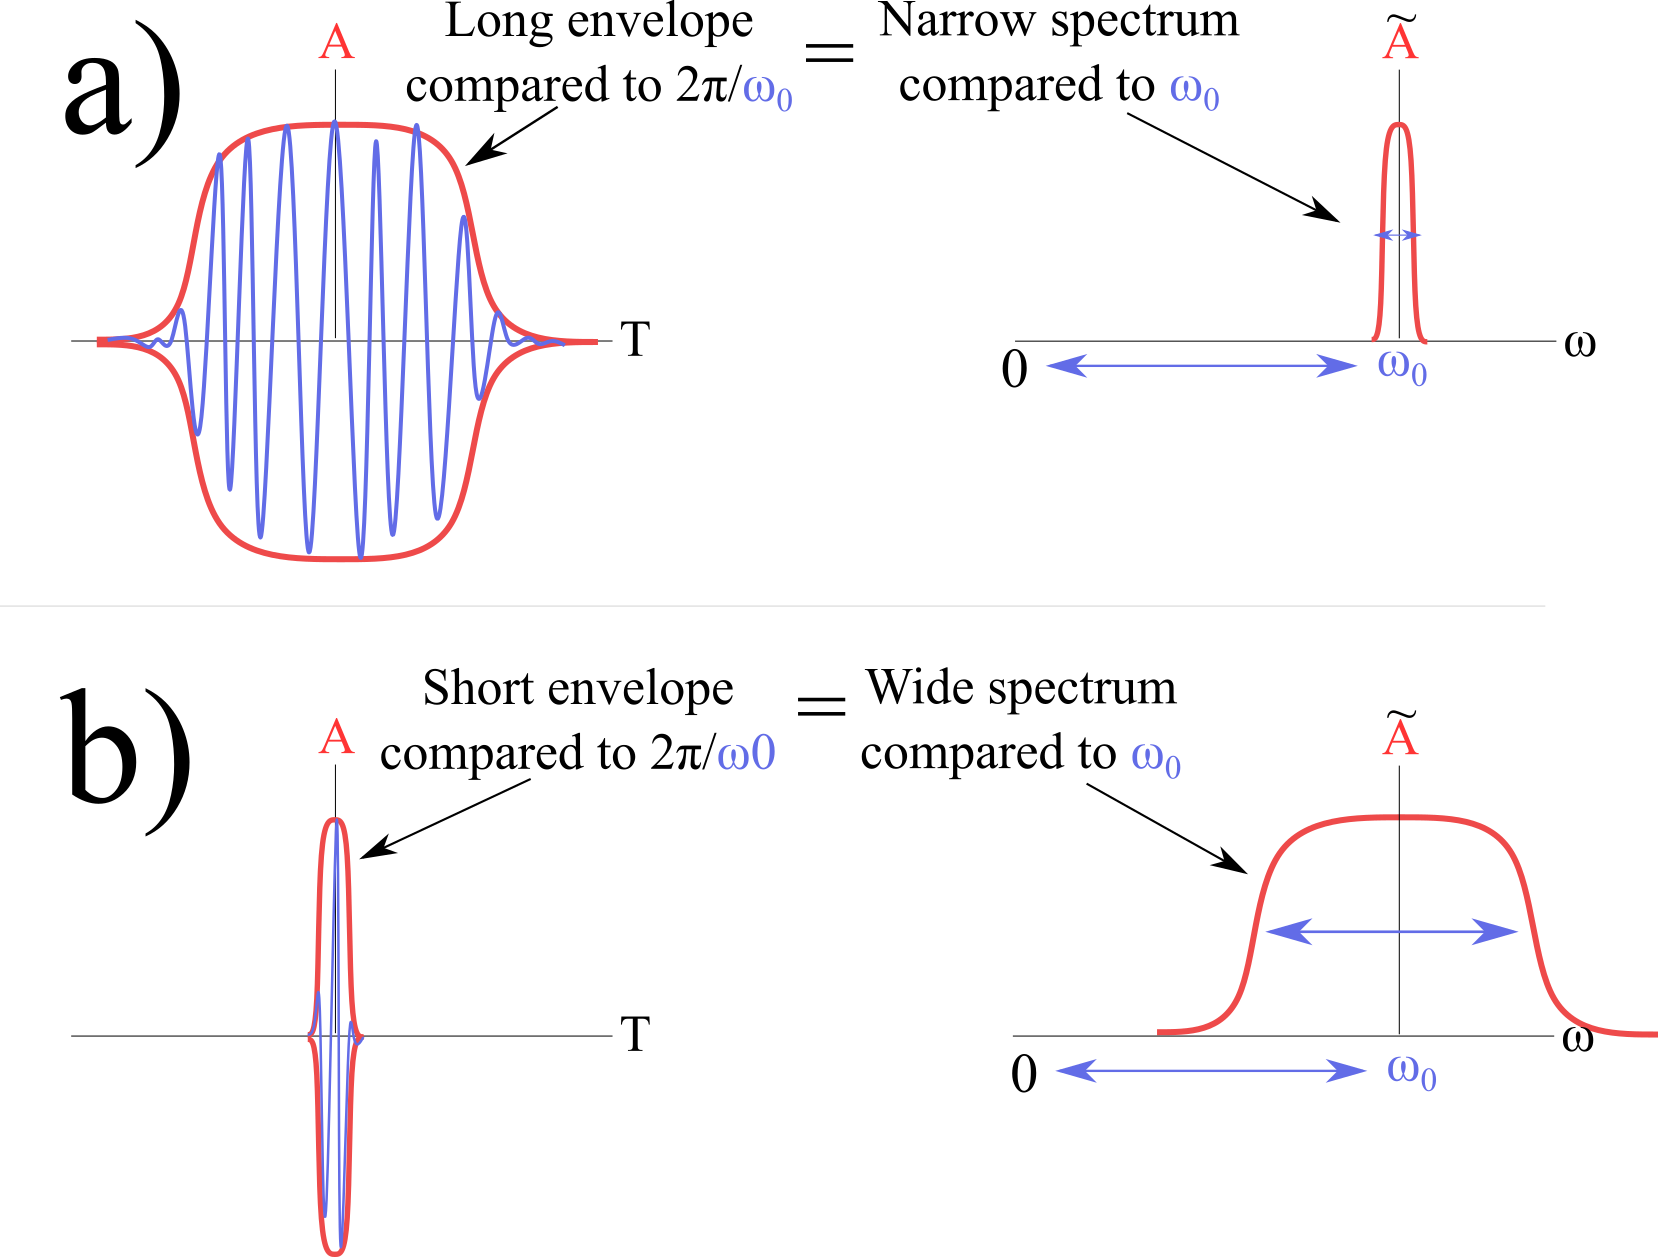
\includegraphics[width=1\linewidth]{figures/bandwidth.png}
    \caption{a) 与载波频率下单次电场振荡的持续时间相比,持续时间长的脉冲频谱较窄。 b)相反,短脉冲的频谱较宽。}
    \label{fig:bandwidth}
\end{figure}

根据这些假设,脉冲的频谱宽度非常窄,以至于 $\betag(\omega)$ 可以围绕载波频率泰勒展开为

\begin{align}
\label{eq:beta_approx}
    \betag(\omega)&\approx \betag(\omega_0)+\partial_\omega\betag|_{\omega_0}(\omega-\omega_0)+\frac{1}{2!}\partial^2_\omega\betag|_{\omega_0}(\omega-\omega_0)^2+
    \frac{1}{3!}\partial^3_\omega\betag|_{\omega_0}(\omega-\omega_0)^3+... \\ \nonumber
    &= \sum_{n=0}^{\infty} \frac{1}{n!}\partial^n_\omega\betag|_{\omega_0}(\omega-\omega_0)^n\\ \nonumber
    &=\sum_{n=0}^{\infty} \frac{1}{n!}\betag_n(\omega-\omega_0)^n.
\end{align}

考虑到这一简化,脉冲在介质中传播的表达式变为

\begin{align}
\label{eq:beta_approx_applied}
    \E(z,t) &= \frac{1}{2\pi}\int_{-\infty}^{\infty} \Tilde{\E}(z,\omega) e^{i(\betag_0+\betag_1(\omega-\omega_0)+\frac{1}{2}\betag_2(\omega-\omega_0)^2+...)z-i\omega t} d\omega.
\end{align}


\section{$\betag_0$ - 载波的延迟程度}

%Because the term containing $\betag_0$ does not depend on $\omega$, it can be moved outside the integral in Eq.~\ref{eq:beta_approx_applied}. Multiplying by $1=\exp(-i\omega_0t)\exp(i\omega_0t)$ yields
由于包含 $\betag_0$ 的项不依赖于 $\omega$,它可以移到公式 ~\ref{eq:beta_approx_applied} 的积分之外。乘以 $1=\exp(-i\omega_0t)\exp(i\omega_0t)$ 得到

\begin{align}
\label{eq:beta_approx_applied}
    \E(z,t) &= \frac{1}{2\pi} e^{i\betag_0z-i\omega_0t}  \int_{-\infty}^{\infty} \Tilde{\E}(z,\omega) e^{i(\betag_1(\omega-\omega_0)+\frac{1}{2}\betag_2(\omega-\omega_0)^2+...)z-i(\omega-\omega_0) t} d\omega.
\end{align}

积分外的指数意味着,如果观察介质中的复数电场,其持续时间为载波的几个周期,那么它看起来就像一个复数平面波,其时间频率为 $\omega_0$,空间频率为 $\betag_0$。关于 $\betag_0$ 对真实平面波在介质中传播的影响,请参见 \href{https://www.desmos.com/calculator/ausd1wnl2j}{此交互式图表}。

\subsection{相速度}
\label{sec:Phase_velocity}

当 $\betag_0z-\omega_0t$ 是 $2\pi$ 的整数倍时,载波将达到峰值。为简单起见,考虑与 $\betag_0z-\omega_0t=0$ 相对应的峰值。如果时间前进了 $0<Delta t$,$z$ 的原始值就不满足 $\betag_0z-\omega_0(t+\Delta t)=0$ 。相反,峰值会出现在某个新的位置 $z+\Delta z$,其中

\begin{align}
    \betag_0(z+\Delta z)-\omega_0(t+\Delta t)=0\\ \nonumber
    \betag_0\Delta z-\omega_0\Delta t=0.
\end{align}

由于峰值在 $\Delta t$ 时间内移动了 $\Delta z$,我们可以将 “相位速度”(或 “载波速度”)定义为

\begin{align}
\label{eq:Phase_velocity}
    v_p &= \frac{\Delta z}{\Delta t} = \frac{\omega_0}{\betag_0}.
\end{align}


\section{$\betag_1$ - 以载波为中心的脉冲包络延迟的程度}

式 ~\ref{eq:beta_approx_applied} 中的积分表示通过介质传播的复电场的包络。对指数项进行重排,可以得到

\begin{align}
\label{eq:envelope_beta1}
    \E(z,t) &= \frac{1}{2\pi} e^{i\betag_0z-i\omega_0t}  \int_{-\infty}^{\infty} \Tilde{\E}(z,\omega) e^{i\betag_1(\omega-\omega_0)z-i(\omega-\omega_0) t} e^{i(\frac{1}{2}\betag_2(\omega-\omega_0)^2+...)z} d\omega.
\end{align}

应用公式 ~\ref{eq:Phase_velocity} 后面的相同分析,我们会发现复电场包络的峰值以所谓的 “群速度”(或 “包络速度”)传播,其值为

\begin{align}
\label{eq:group_velocity}
    v_g &= \frac{(\omega-\omega_0)}{\betag_1\cdot(\omega-\omega_0)} = \frac{1}{\betag_1} = \frac{1}{\partial_\omega\betag}.
\end{align}

关于相位速度和群速度之间的区别,请参见 \href{https://www.desmos.com/calculator/rq2physwac}{此交互式图表}。请注意,公式~\ref{eq:group_velocity}与公式~\ref{eq:delay_definition}的预测一致,即相位相对于 $\omega$ 发生较大的正向变化应导致较大的延迟。




\section{$\betag_2$ - 构成以载波为中心的脉冲包络的频率相对延迟的程度}

\label{sec:GVD}

将公式 ~\ref{eq:envelope}应用于公式 ~\ref{eq:envelope_beta1},可以 “剔除 ”载波快速但可预测的空间和时间振荡,将注意力集中在包络上:

\begin{align}
    \A(z,t)  &= \frac{1}{2\pi}  \int_{-\infty}^{\infty} \Tilde{\A}(z,\omega) e^{i\betag_1(\omega-\omega_0)z-i(\omega-\omega_0) t} e^{i(\frac{1}{2}\betag_2(\omega-\omega_0)^2+...)z} d\omega.
\end{align}

为了进一步简化,我们可以定义 $T=t-\betag_1z$,即 “脉冲包络到达距离 $z$ 时的相对时间”。使用 $T$ 代替 $t$ 是很方便的,因为许多光学实验都需要发送脉冲光穿过固定长度的介质,并跟踪光离开介质后一段时间内测量到的功率:   

\begin{align}
    \A(z,T)  &= \frac{1}{2\pi}  \int_{-\infty}^{\infty} \Tilde{\A}(z,\omega) e^{i\betag_1(\omega-\omega_0)z-i(\omega-\omega_0) (T+\betag_1z)} e^{i(\frac{1}{2}\betag_2(\omega-\omega_0)^2+...)z} d\omega \\ \nonumber
    &= \frac{1}{2\pi}  \int_{-\infty}^{\infty} \Tilde{\A}(z,\omega) e^{i(\frac{1}{2}\betag_2(\omega-\omega_0)^2+...)z-i(\omega-\omega_0)T} d\omega.
\end{align} 

正如公式 ~\ref{eq:spectrum_time_example}所解释的那样,$\betag_2$ 的正值(负值)意味着较低的(较高的)时间频率比较高的(较低的)时间频率传播得更快,从而导致脉冲包络在时域中变宽。或者,我们也可以考虑只包含 $\betag_2$ 项的公式 ~\ref{eq:GNLSE}、

\begin{align}
    \label{eq:heat_equation}
    \partial_z \A = -i  \frac{\betag_2}{2}\partial_T^2\A,
\end{align}

这与所谓的 “热方程 ”相同 ~\cite{Fourier_heat_original,Fourier_heat_english}. 参见 
\href{https://digitalcommons.ursinus.edu/cgi/viewcontent.cgi?article=1008&context=triumphs_differ}{本教程}。为了得到 $\A(z,T)$ 给定的 $\A(z=0,T)$ 以及 $\tilde{A}(z=0,\omega)$ ,首先计算公式的傅立叶变换 ~\ref{eq:heat_equation} 以得到

\begin{align}
    \label{eq:beta2_broadening}
    \partial_z \Tilde{\A} &= -i  \frac{\betag_2}{2} (i(\omega-\omega_0))^2 \Tilde{\A} \\ \nonumber
    &= i  \frac{\betag_2}{2}(\omega-\omega_0)^2\Tilde{\A} \\ \nonumber
    \Tilde{\A}(z,\omega)&=\Tilde{\A}(0,\omega)e^{i\frac{\betag_2}{2}(\omega-\omega_0)^2z} \\ \nonumber
    \A(z,T) &= \IFT\left\{  \Tilde{\A}(z,\omega)   \right\}.
\end{align}

对于高斯脉冲,公式(~\ref{eq:beta2_broadening})可以通过(\href{https://drive.google.com/file/d/17Ab3bg0Hx0x8J-5lR29ejFg0eOlv6Psh/view?usp=sharing}{分析})求解。结果确实意味着脉冲会在时间上变宽,而将公式\ref{eq:chirp_definition}应用于结果则证实,$\betag_2>0$ 意味着低频将比高频更早到达。由于$\betag_2$引起的相位偏移的大小随着给定频率分量与载波之间距离的增加而呈二次增长,因此在相同距离内,频谱宽度较大的短脉冲将比带宽较小的短脉冲在时间上更宽。由 $\betag_2$ 导致的增宽变得显著的特征长度可定义为

\begin{align}
    \label{eq:Dispersion_length}
    L_{2} &= \frac{T_0^2}{|\betag_2|}.
\end{align}

有关色散对高斯脉冲的影响,请参阅 \href{https://www.youtube.com/watch?v=BP6Ra98AEuU}{本视频}。

\subsection{零色散频率}
\label{subsec:ZDF}

对于已知 $\betag(\omega)$ 的给定介质,可以计算出给定载波频率 $\omega_0$ 附近的 $\betag_2$ 值为

\begin{align}
\label{eq:ZDF}
    \betag_2(\omega) &= \betag_2|_{\omega=\omega_0} + \betag_3|_{\omega=\omega_0}\cdot(\omega-\omega_0)+\frac{1}{2}\betag_4|_{\omega=\omega_0}\cdot(\omega-\omega_0)^2 +...,
\end{align}

这样就可以求解特定频率(或者说复数频率!),$\omega_{ZD}$,其中$\betag_2(\omega_{ZD})=0$。这个 “零色散频率 ”非常重要,因为很多非线性机制在 $\omega_{ZD}$ 或接近 $\omega_{ZD}$ 的频率下会更有效,其中 $\betag_2<0$。因此,在进行非线性光学实验时,确定特定介质的 $\omega_{ZD}$ 值至关重要。特定光纤的零色散频率可以使用常见的光学实验室设备进行实验测量~\cite{zero_disp_measurement}。
从历史上看,用于电信的光纤被设计成接近激光的近红外频率($\approx$190-230~THz $\approx$1310-1550~nm),易于产生、调制和检测。这样做的目的是为了防止携带数字信息的脉冲出现时间展宽、重叠和干扰。自 2000 年代中期以来,电子色散补偿技术的进步使这种光纤设计变得过时甚至有害,因为非线性效应会通过改变信号的相位和振幅来扭曲信号,在接近 $\omega_{ZD}$ 时这种效应更为显著。

\section{$\betag_n$ - 高阶延迟}

在理解了$\betag(\omega)$(即$\betag_1$)的斜率决定脉冲包络的传播速度,而$\betag(\omega)$(即$\betag_2$)的曲率决定脉冲的时间展宽之后,这些见解可以得到推广。例如,$\betag_3>0$ 意味着$i\betag_3/6(\omega-\omega_0)^3z$ 项会导致除载波外所有频率的正$\partial_\omega\phi$。因此,对脉冲有贡献的高频和低频都会开始落后于主脉冲,从而导致不对称的时间展宽。此外,$\betag_4>0$意味着$i\betag_4/24(\omega-\omega_0)^4z$会在$\betag_2$引起的时间展宽之外引起额外的对称时间展宽。请参见图 ~\ref{fig:dispersion_combined},了解不同的 $\betag_n$ 项对高斯脉冲时间轮廓的影响。在分析脉冲在介质中传播的演化时,$\betag(\omega)$ 的扩展中包含多少项取决于脉冲的频谱宽度,而频谱宽度与其持续时间成反比。对于 1~ps 以上的脉冲,高于 $\betag_3$ 的阶数很少有贡献。在用持续时间为 10~fs 的脉冲对超连续产生进行数值模拟时,为了稳妥起见,通常会包含高达 $\betag_8$ 的阶次。与公式~\ref{eq:Dispersion_length}类似,高阶色散效应变得显著的特征长度定义为

\begin{align}
\label{eq:dispersion_length_general}
    L_{n} &= \frac{T_0^n}{|\betag_n|}.
\end{align}

有关色散的更多详情,请参阅 \href{https://www.youtube.com/watch?v=E3S0BQiy3p8&ab_channel=YourFavouriteTA}{本视频教程}。


\section{$\alpha(\omega)$ 和 $\betag(\omega)$ 是独立的吗?}
\label{sec:KK_relations}

在公式~\ref{eq:GNLSE}中,$\alpha$被视为常数,因为在典型脉冲的带宽范围内,其频率依赖性通常很弱。然而,原则上我们可以像对待 $\betag(\omega)$ 一样,对 $\alpha(\omega)$ 进行泰勒展开。有趣的是,我们发现对于给定介质来说,函数 $\alpha(\omega)$ 和 $\betag(\omega)$ 是通过所谓的 \href{https://en.wikipedia.org/wiki/Kramers%E2%80%93Kronig_relations#Related_proof_from_the_time_domain}{克莱默斯-克罗尼格关系(Kramers-Kronig Relations)} 相互关联的,知道其中一个就可以计算另一个。因此,$\alpha(\omega)$ 和 $\betag(\omega)$ 不能独立选择。从数学上证明这种联系很困难,但从物理上来说,直觉告诉我们,与频率相关的$\alpha(\omega)$吸收从根本上说正是产生与频率相关的相位延迟$\betag(\omega)$的原因。此外,介质在给定位置对外加电场的响应只能取决于该位置电场的当前和过去的值,这进一步限制了衰减和相位延迟的组合。方便的是,如果将 $\alpha(\omega)=\alpha$ 视为频率常数,那么它的值可以自由改变,而不会影响 $\betag_n$ 的任何值。 

有关克拉默-克罗尼格关系的更多详情,请参见 \href{https://www.youtube.com/watch?v=vzBnsG2rKWs}{视频一 } 和 \href{https://www.youtube.com/watch?v=rFTUTxPHYYw}{视频二}。请参阅 \href{https://www.desmos.com/calculator/1zymtgbbrv}{这个交互图},了解在时域中使用因果关系和克拉默-克罗尼格关系将 $\alpha(\omega)$ 与 $\betag(\omega)$ 联系起来的教程。


\begin{figure}
    \centering
    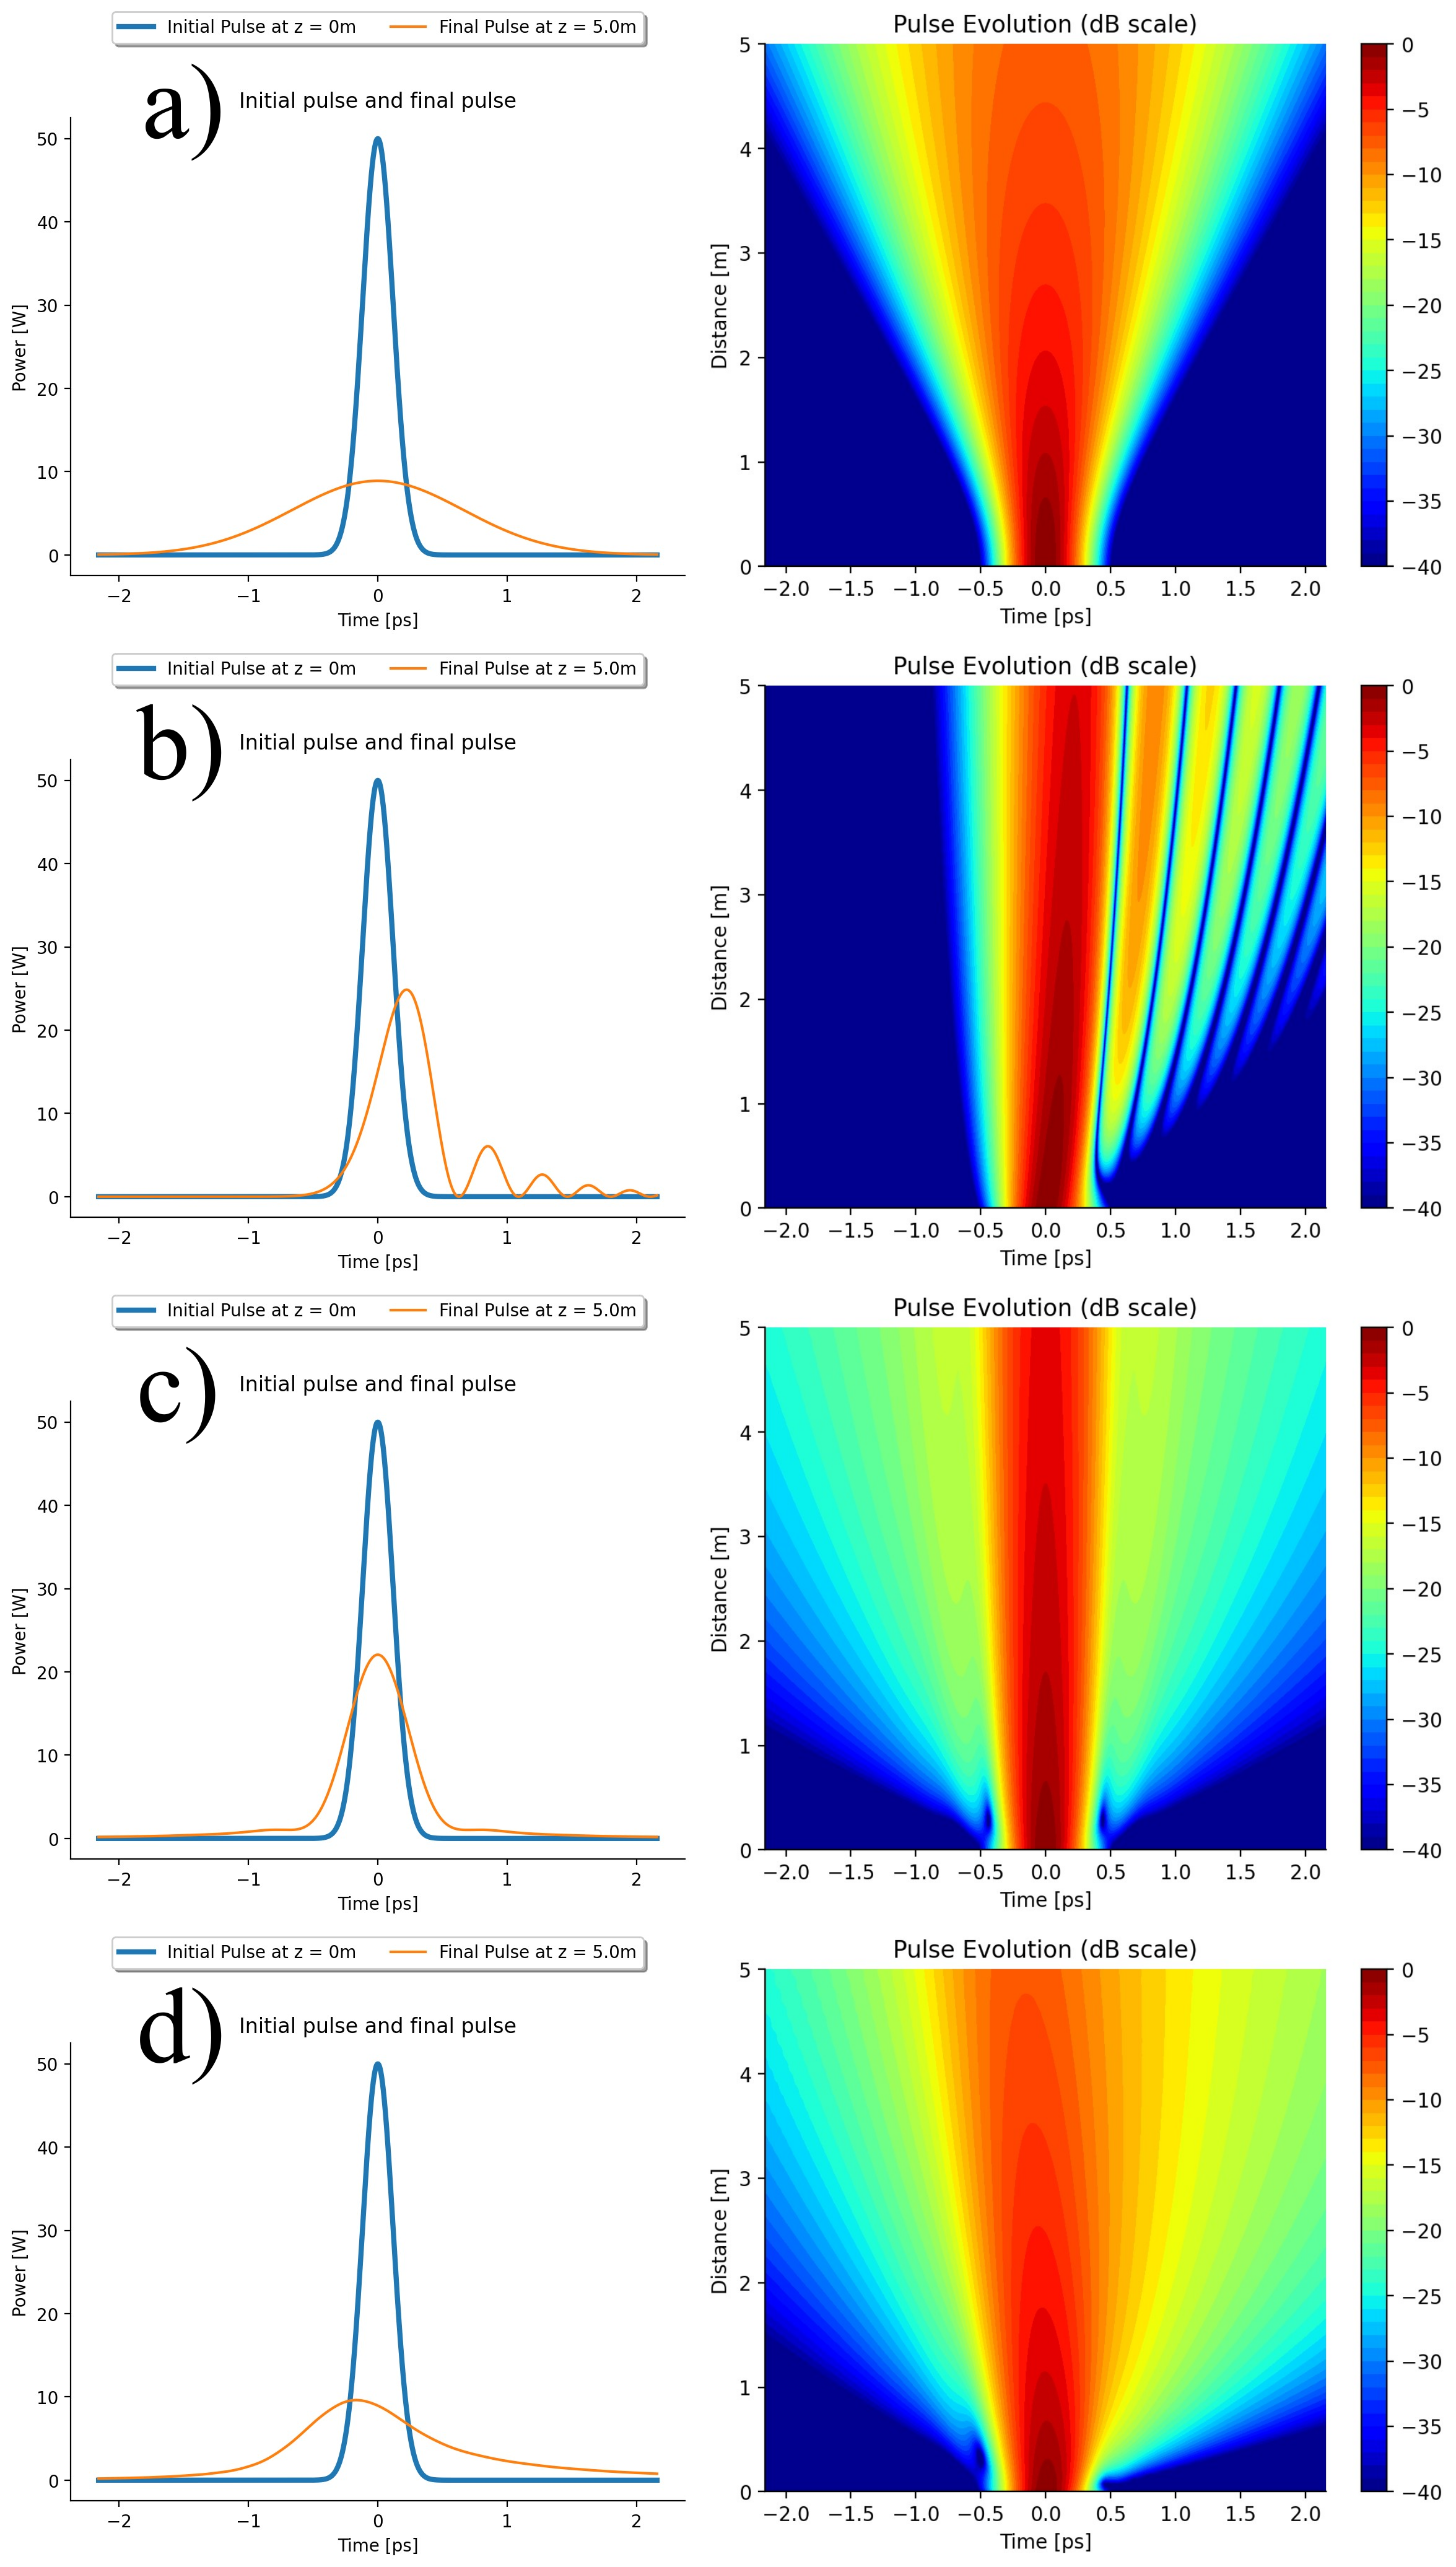
\includegraphics[width=0.75\linewidth]{figures/dispersion_combined.png}
    \caption{时域中不同 $\betag_n$ 项对高斯脉冲的影响说明。左栏显示了脉冲在不同$\betag_n$项介质中传播前后的功率包络对比。右栏显示的是功率包络随距离的变化。  a) $\betag_2<0$ 的介质; b) $\betag_3>0$ 的介质; c) $\betag_4<0$ 的介质; d) 同时存在 $\betag_2<0$ 、 $\betag_3>0$ 和 $\betag_4<0$ 的介质。
    使用 \href{https://colab.research.google.com/drive/1PW9smFA3PECvcXyWpZcW1ogY4W3hEYFt?usp=sharing}{这个可交互notebook} 中的数值模拟生成。我们鼓励读者尝试使用。}
    \label{fig:dispersion_combined}
\end{figure}
    \chapter{自相位调制}
\label{ch:SPM}

在具有三阶非线性的材料中,某一时刻的折射率取决于该时刻的光功率。因此,与低功率但形状相同的脉冲相比,高功率脉冲将经历更大的相位变化。由于非线性介质中可以同时存在不同频率的光,描述非线性对光场的影响可能较为复杂。本章解释了一个简单的情况,即“自相位调制”(SPM),其中仅存在一个以单一载频为中心的脉冲。

\section{脉冲中的相位变化}
从方程~\ref{eq:GNLSE}出发,并假设除$\gamma>0$之外的所有参数都为零,$\omega_0\A\gg\partial_T\A$,且$R(T_{delay})=\delta(T_{delay})$,则广义非线性薛定谔方程简化为
\begin{align}
\label{eq:SPM}
    \partial_z\A &= i\gamma|\A|^2\A.
\end{align}
从数学角度看,方程~\ref{eq:SPM}表明,对于$z$的微小变化,复数$\A$的变化量等于其自身在复平面上旋转90度($i\A$),并根据其自身的平方模($|\A|^2$)以及标量$\gamma$进行缩放。从物理角度看,方程~\ref{eq:SPM}暗示非线性效应会根据功率改变场的瞬时相位,但不会改变该瞬时的功率大小。解方程~\ref{eq:SPM}得到
\begin{align}
    \label{eq:SPM_applied}
    \A(z,T)&= \A(0,T)\exp\left( i\gamma|\A(0,T)|^2z \right).
\end{align}
为了理解方程~\ref{eq:SPM_applied}的含义,可以参考方程~\ref{eq:chirp_definition},该方程指出脉冲的瞬时频率与其相位相对于时间的负导数有关。假设一个高斯脉冲$\A(0,T)=\A_0\exp(-T^2/2T_0^2)$,则该脉冲在通过非线性介质传播距离$z$后的瞬时频率为
\begin{align}
\label{eq:SPM_example}
    \delta\omega(z,T) &= -\gamma |\A_0|^2 z\partial_T \exp\left(-\frac{T^2}{T_0^2}\right)\\ \nonumber
    &= 2\gamma |\A_0|^2 z T/T_0^2 \exp\left(-\frac{T^2}{T_0^2}\right),
\end{align}
这表明脉冲前沿将产生红移,后沿将产生蓝移。参见图~\ref{fig:chirp_profiles}(a)以了解高斯脉冲产生的啁啾可视化,参见图~\ref{fig:chirp_profiles}(b-d)以了解其他脉冲形状产生的啁啾。考虑方程~\ref{eq:SPM_applied}中指数的参数,可定义非线性效应变得显著的特征长度为
\begin{align}
    L_{NL} &= \frac{1}{\gamma P_0} = \frac{1}{\gamma |\A(0,T)|^2},  
\end{align}
其中$P_0$为脉冲的初始峰值功率。

\begin{figure}
    \centering
    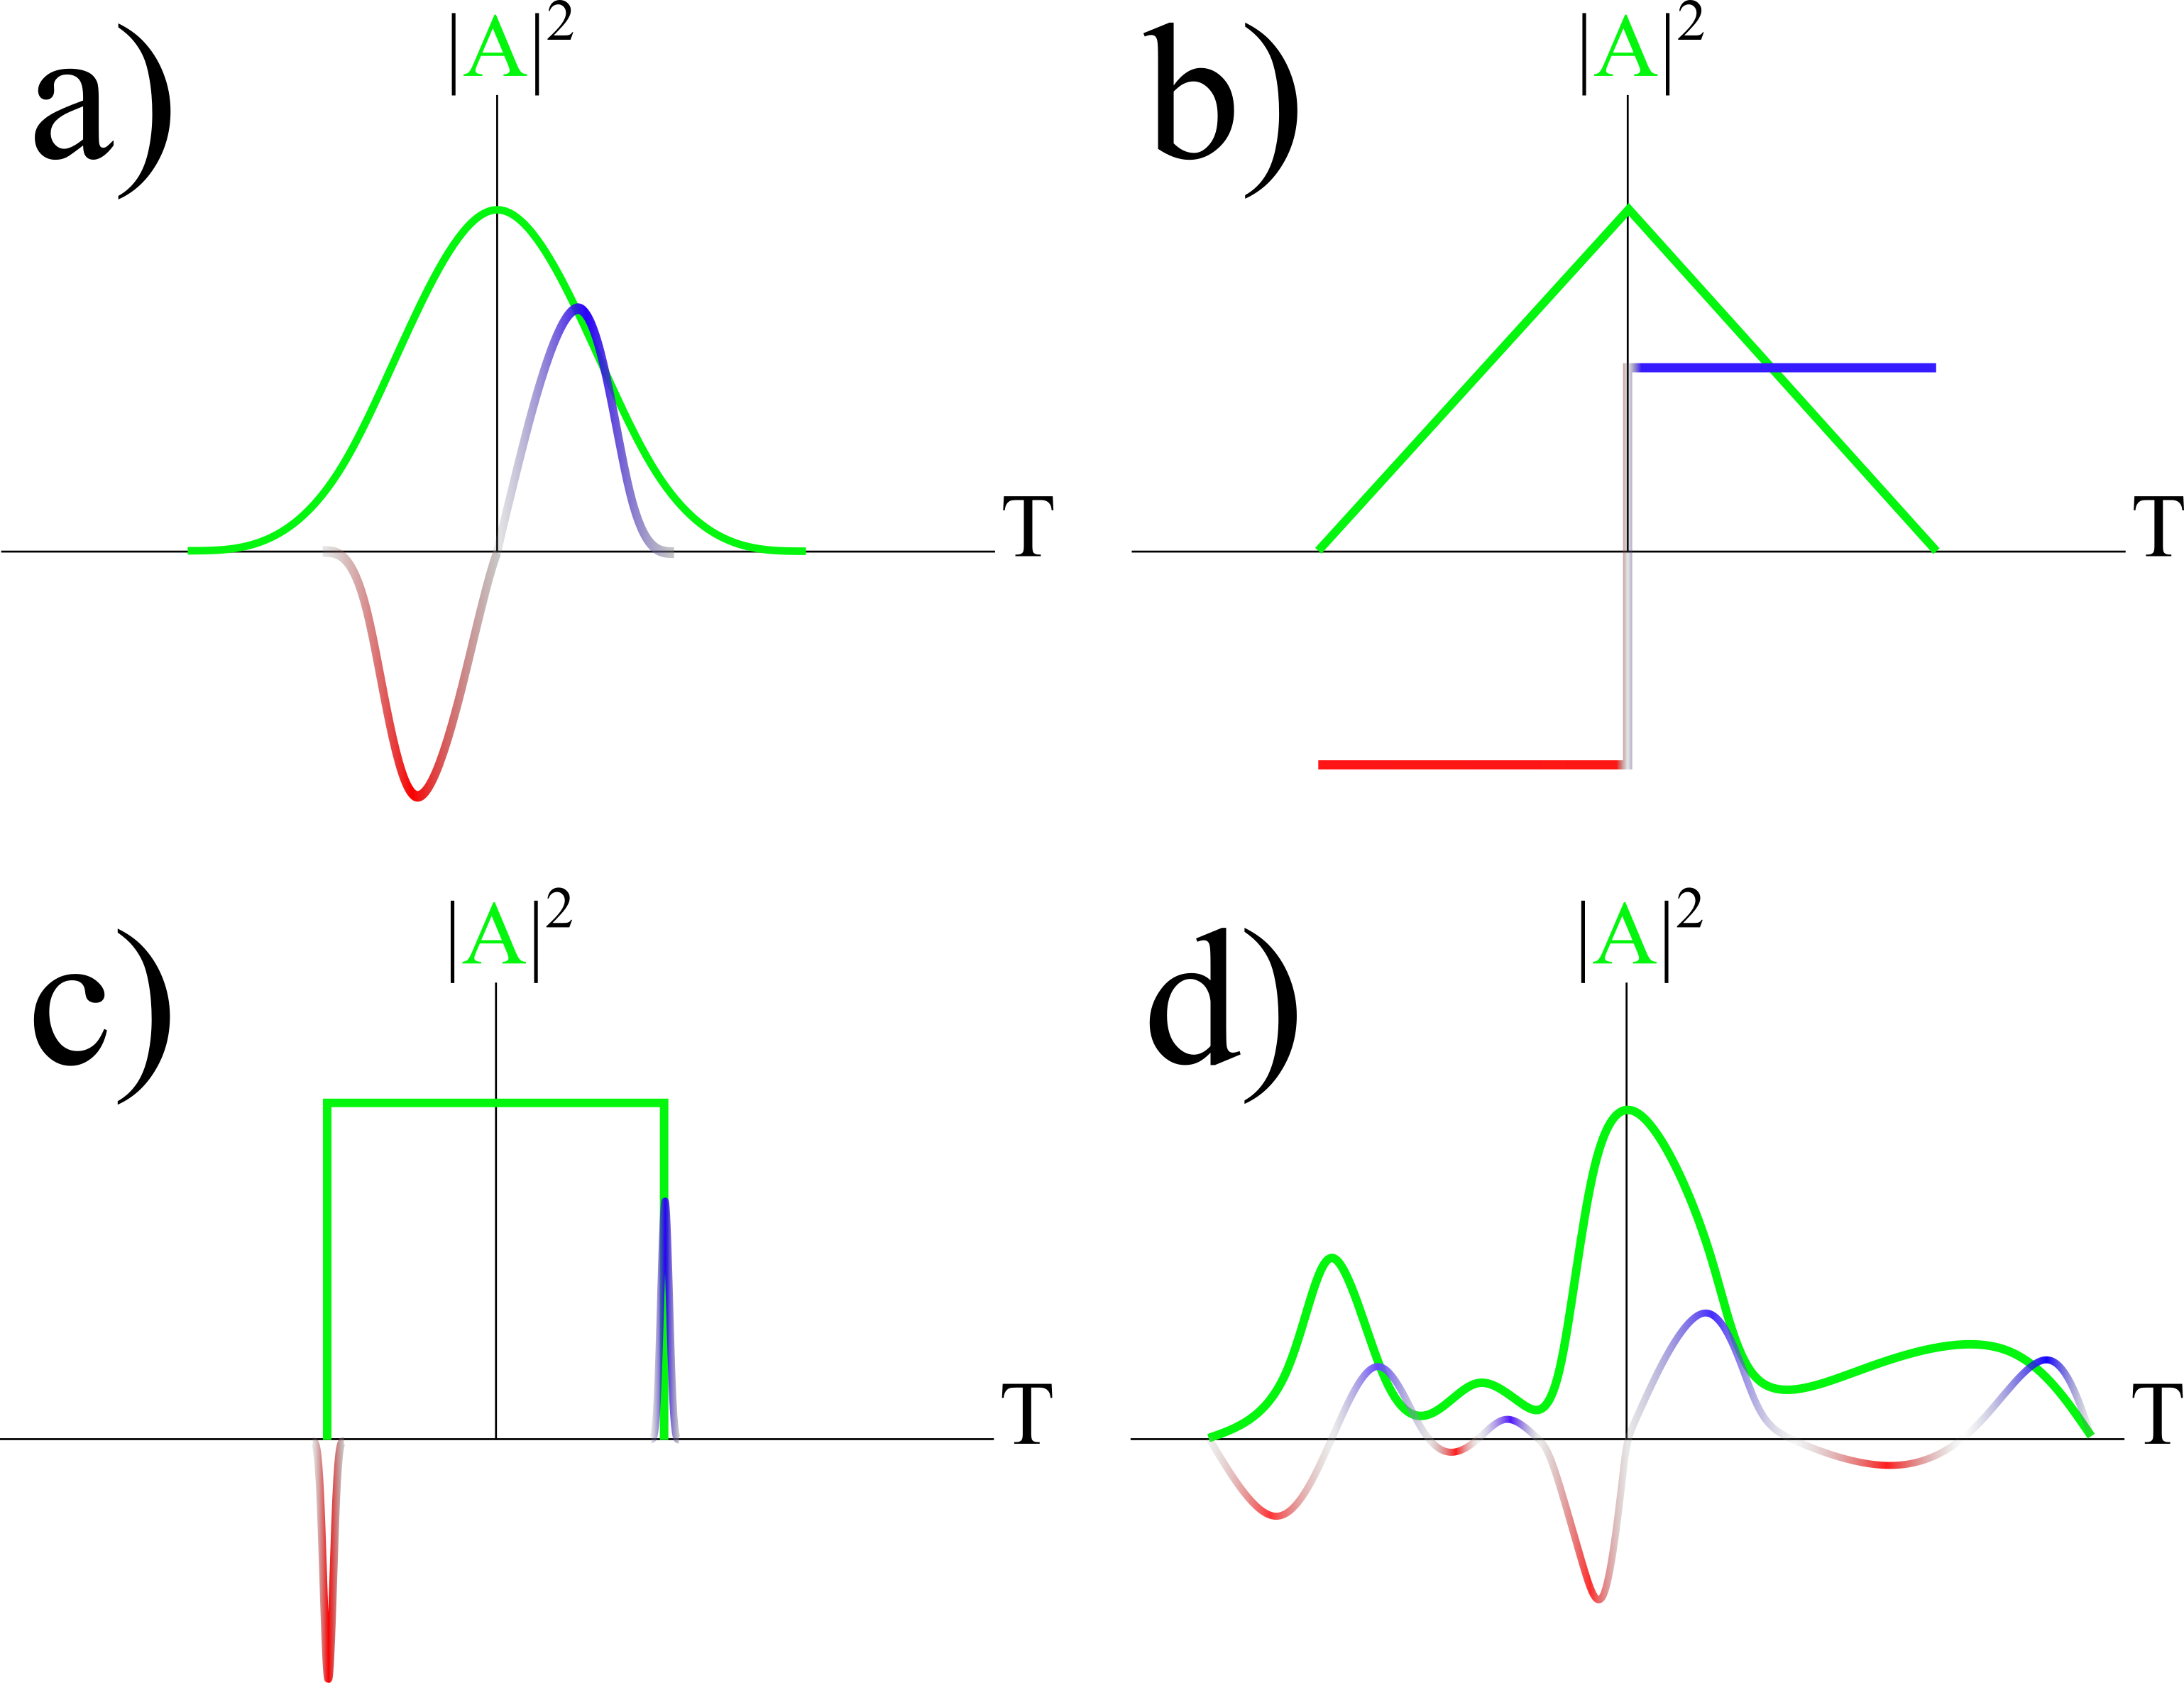
\includegraphics[width=0.75\linewidth]{figures/SPM_chirp.png}
    \caption{SPM对(a)高斯脉冲,(b)三角脉冲,(c)方波脉冲,(d)任意脉冲的影响可视化。一般来说,正斜率会导致红移啁啾,负斜率导致蓝移啁啾,水平斜率则不会产生啁啾。}
    \label{fig:chirp_profiles}
\end{figure}

\section{谱展宽}
对等式~\ref{eq:SPM_example}的分析表明,自相位调制(SPM)会导致脉冲在前导坡度上变得“更红”,在后导坡度上变得“更蓝”。单独考虑时,$\betag_2>0$也会导致类似的行为,但关键区别在于,色散仅改变不同频率分量的相对相位,而SPM还会改变它们的幅度。换句话说,作用在脉冲上的SPM会产生新的颜色,这些颜色在最初并不存在!通过对等式~\ref{eq:SPM}两边进行傅里叶变换可以从数学上看到,这意味着在频谱域中的展宽,因为傅里叶变换在时域中两个函数的乘积等效于频域中的卷积:

\begin{align}
\label{eq:SPM_freq}
    \partial_z\Tilde{\A} &= i\gamma \FT\left\{\A\A^*\A\right\} \\ \nonumber
    &= i\gamma \Tilde{\A}*\Tilde{\A^*}*\Tilde{\A}.
\end{align}

简而言之,等式~\ref{eq:SPM_freq} 表明 $\A$ 的频谱相对于 $z$ 的变化取决于其频谱与自身及其复共轭的卷积。由于卷积两个函数会产生一个比初始函数更宽的函数,等式~\ref{eq:SPM_freq}显示频谱将随距离的增加而展宽,暗示通过将功率从载波向红、蓝端转移而添加新频率。请参见图~\ref{fig:SPM_before_and_after},了解SPM对高斯脉冲的影响示例。

\begin{figure}
    \centering
    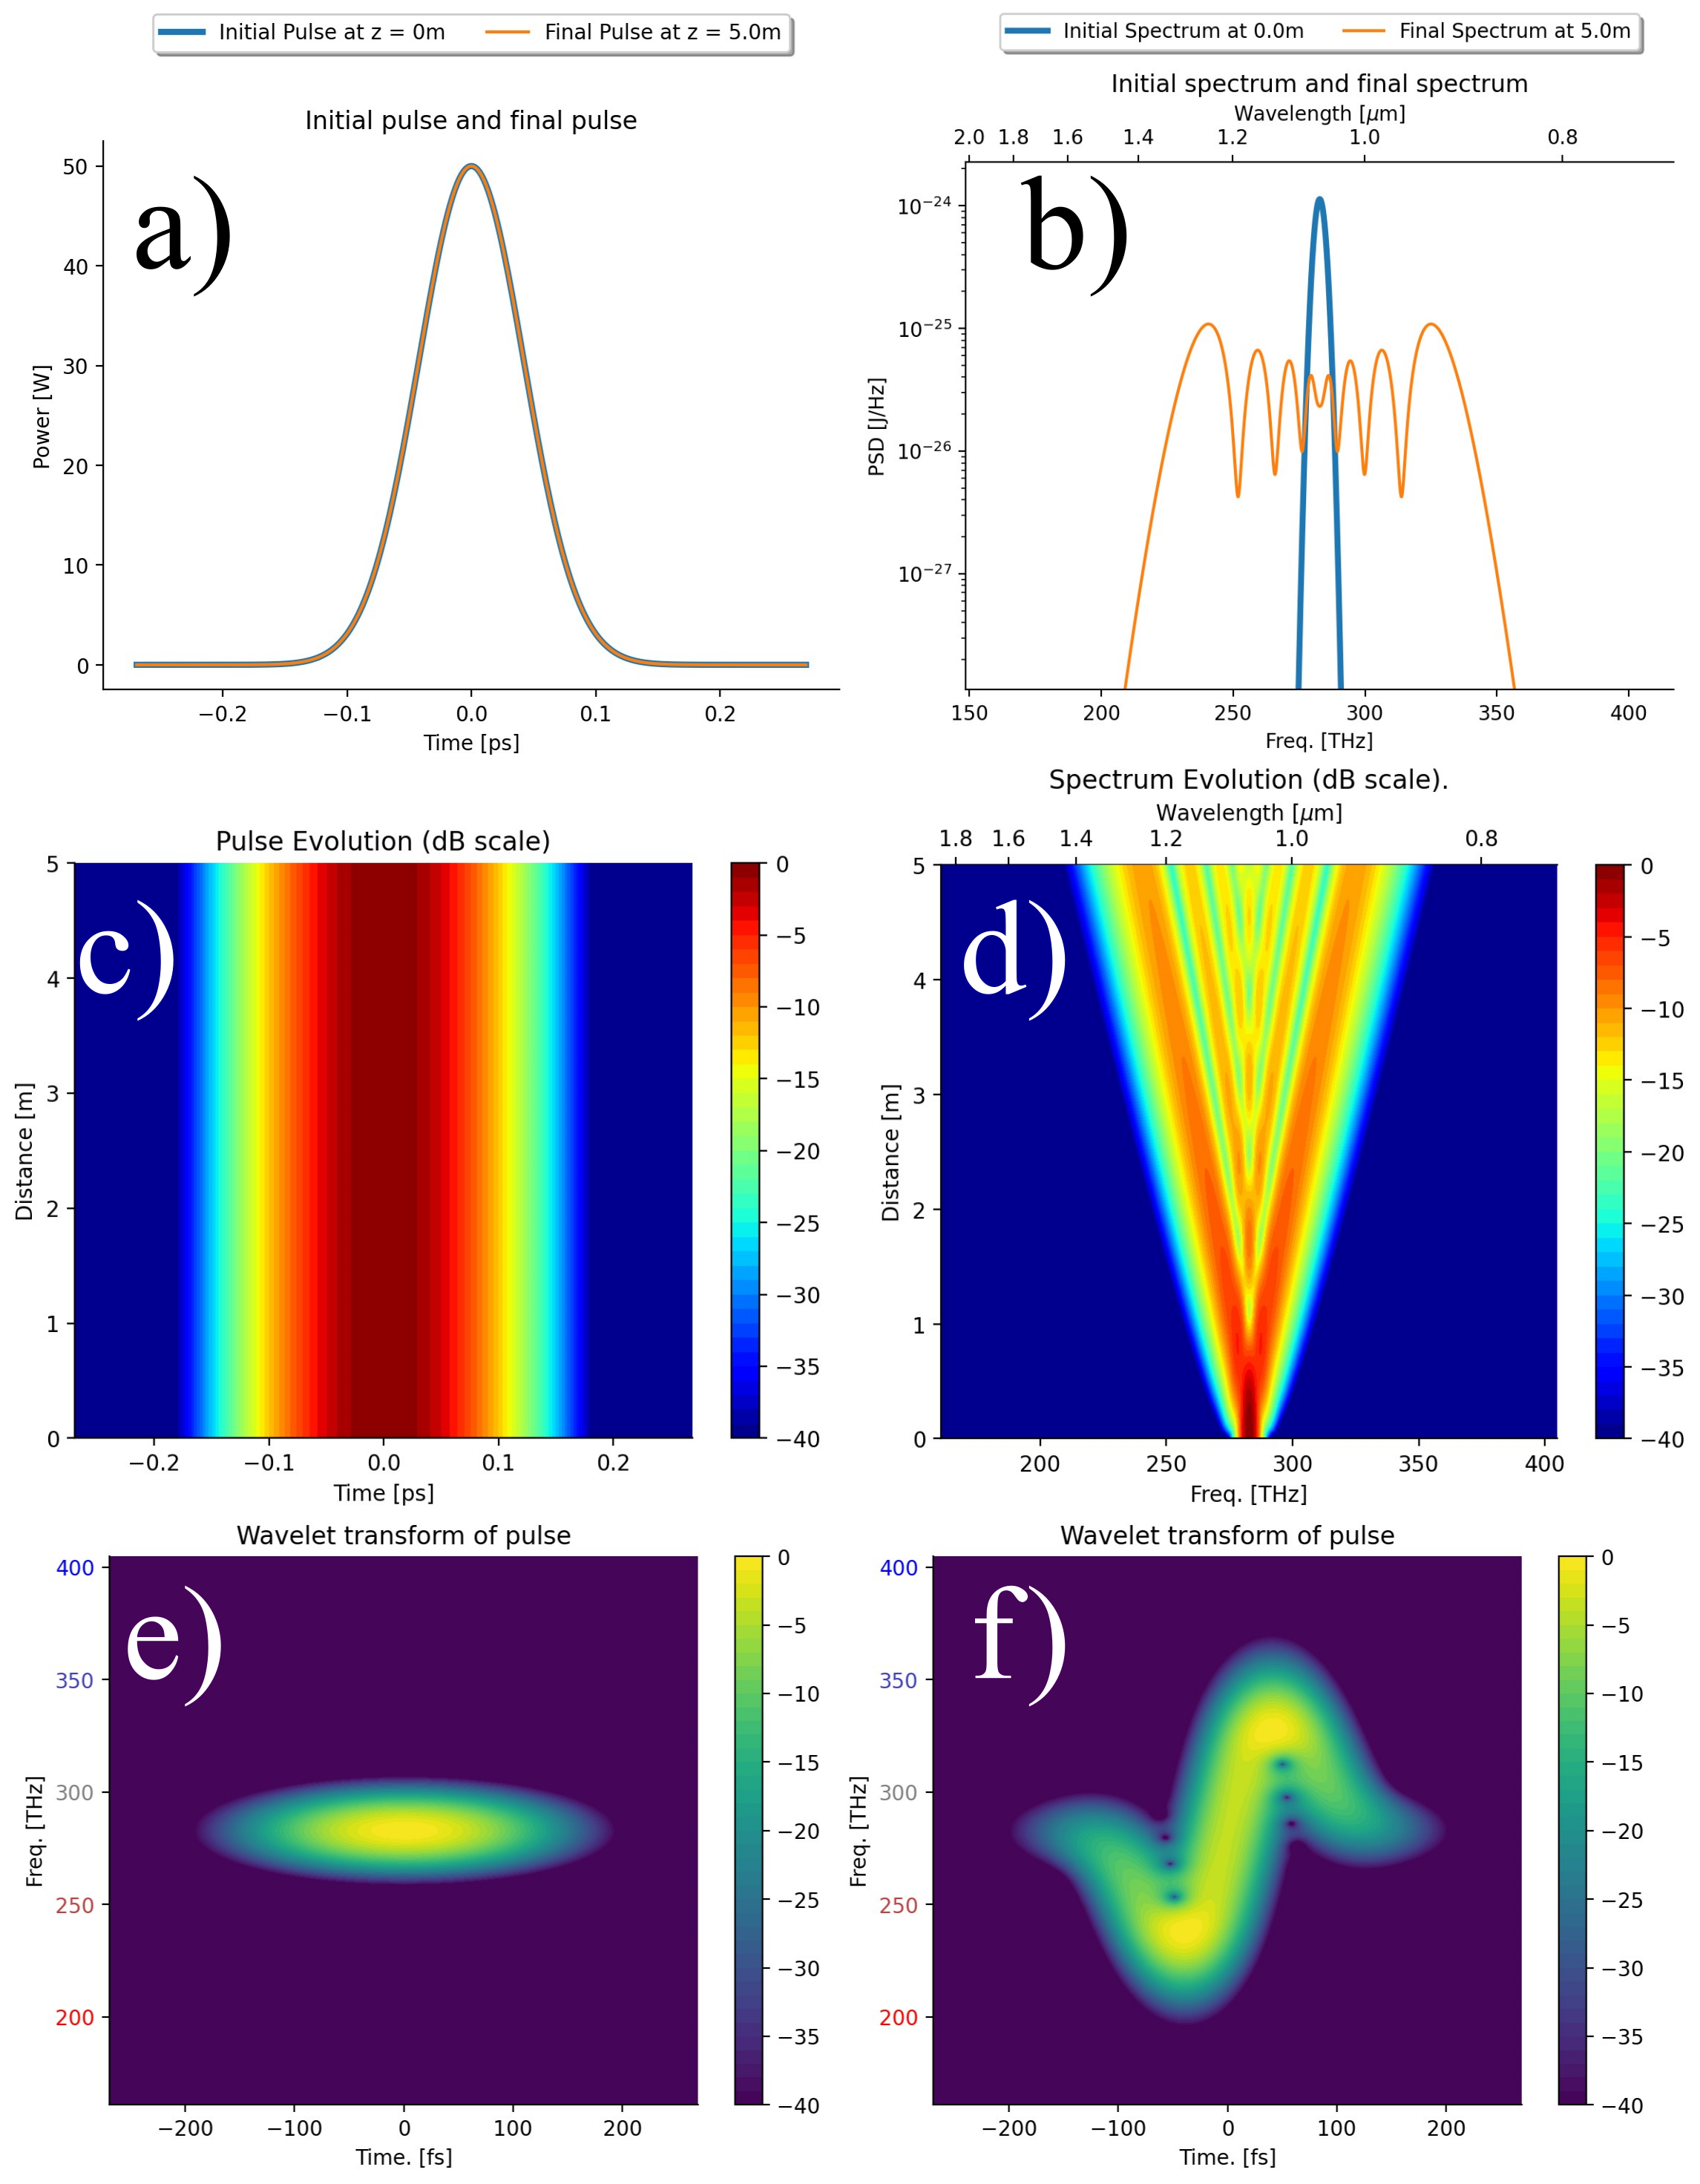
\includegraphics[width=1\linewidth]{figures/SPM_combined.png}
    \caption{ 高斯脉冲在由等式~\ref{eq:SPM}描述的非线性介质中传播的前后对比。
    a) 在时域中,脉冲的功率包络保持不变。 b) 频谱展宽。 c) 时域中功率包络的演化没有变化。 d) 频谱逐渐展宽。 e) 传播前的脉冲频谱图。 f) 传播后的脉冲频谱图。请注意频谱域中的展宽以及时间域中宽度的恒定。使用\href{https://colab.research.google.com/drive/1P41F4hO6Mv12RsEkpogYv5teQyFZ6iW0?usp=sharing}{这个交互notebook}中的数值模拟生成图形,读者可以尝试进行实验。}
    \label{fig:SPM_before_and_after}
\end{figure}


\section{自相位调制、损耗与“有效长度”}
考虑等式~\ref{eq:GNLSE},假设与等式~\ref{eq:SPM}相同,但此时 $\alpha\neq0$。回忆等式~\ref{eq:attenuation_power},其中 $\alpha\neq0$ 会导致脉冲功率随距离呈指数变化。在这种情况下,

\begin{align}
\label{eq:SPM_and_loss}
    \partial_z\A &= \frac{\alpha}{2}\A +i\gamma|\A|^2\A\\ \nonumber
    &=\left(\frac{\alpha}{2} +i\gamma |\A(0,T)|^2 \exp(\alpha z) \right)\A. 
\end{align}

将等式~\ref{eq:SPM_and_loss} 从 $0$ 积分到 $z$ 得到:

\begin{align}
    \label{eq:Leff_derivation}
    \A(z,T)&=\A(0,T) \exp\left( \frac{\alpha}{2}z+i\gamma|\A(0,T)|^2 \int_0^z \exp(\alpha\xi) d\xi  \right) \\ \nonumber
    &=\A(0,T) \exp\left( \frac{\alpha}{2}z+i\gamma|\A(0,T)|^2  \frac{\exp(\alpha z)-1}{\alpha}   \right) \\ \nonumber
    \A(L,T)&=\A(0,T) \exp\left( \frac{\alpha}{2}z+i\gamma|\A(0,T)|^2  L_{eff}   \right),
\end{align}

其中,具有实际长度 $L$ 的介质的“有效长度”定义为:

\begin{align}
\label{eq:L_eff}
    L_{eff}= \frac{\exp(\alpha L)-1}{\alpha}.
\end{align}

等式~\ref{eq:Leff_derivation} 和等式~\ref{eq:L_eff}提供的见解是,尽管通过让光在更长的介质中传播通常会增强非线性效应,但该介质的损耗最终会使光功率降低到所有非线性效应变得可以忽略的程度。例如,对于典型的100公里长单模光纤(损耗系数为$\alpha=-0.22$dB/km),其有效长度约为19.6公里。换句话说,光信号在100公里有损耗光纤中的非线性相移累积量大致等于在19.6公里无损耗光纤中的累积量。请参见\href{https://www.desmos.com/calculator/g6dadbxq33}{这个互动图表}以查看有效长度如何依赖于 $\alpha$。注意,当 $\alpha L\ll 1$ 时,$L_{eff}\approx L$;而在 $\alpha>0$ 的情况下(如在光放大器中),可能出现 $L_{eff}>L$。此外,$\alpha$ 在特殊的非均匀光纤或存在拉曼放大时可能随 $z$ 而变化,此时需要相应修改等式~\ref{eq:attenuation} 和等式~\ref{eq:SPM_and_loss}。

\section{自陡效应}
\label{sec:SS}

在等式~\ref{eq:SPM}中,假设非线性相位偏移与场包络乘以其平均功率成正比,即 $\A|\A|^2$。这种假设可以视为非线性响应的相对于时间的零阶泰勒近似,类似于将 $\exp(x)\approx 1$ 用于非常小的 $x$。若进一步假设场包络的变化率乘以其平均功率 $\partial_T(\A|\A|^2)$ 也有贡献,则得到:

\begin{align}
\label{eq:SS}
    \partial_z\A &= i\gamma\left(1+\frac{i}{\omega_0}\partial_T \right)\A|\A|^2.
\end{align}

在等式~\ref{eq:SS}中的括号内,第一个项是自相位调制(SPM),而第二个项称为“自陡效应”(SS)。物理上,可以理解为非线性效应导致脉冲高功率部分的折射率发生显著变化。较高的折射率意味着光传播速度更慢,因此高功率脉冲的峰值在传播时比较低强度部分减速,从而在后续时间上积累功率,导致坡度陡降。类似地,一辆大且不流线型的卡车在遇到强逆风时会比流线型汽车大幅减速,从而在后方形成堵塞,而前方交通则较稀疏。由于SS效应平坦化了脉冲前端的功率坡度,并使后端变得陡峭,因此优先将脉冲频谱蓝移,因为 $\delta\omega\propto -\partial_T|\A|^2$。请参见图~\ref{fig:SS},了解SS对与图~\ref{fig:SPM_before_and_after}相同高斯脉冲的影响。对于仅受SPM和自陡效应影响的高斯脉冲,\href{https://prefetch.eu/know/concept/self-steepening/}{可以证明}其后坡在距离

\begin{align}
    L_{SS} &= \frac{T_0\omega_0\exp(1/2)}{3\sqrt{2}\gamma P_0}
\end{align}

处变得无限陡。

更多关于SS的信息,请参考\href{https://youtu.be/Fr6yLtGZ2To}{这个视频教程}。

\begin{figure}
    \centering
    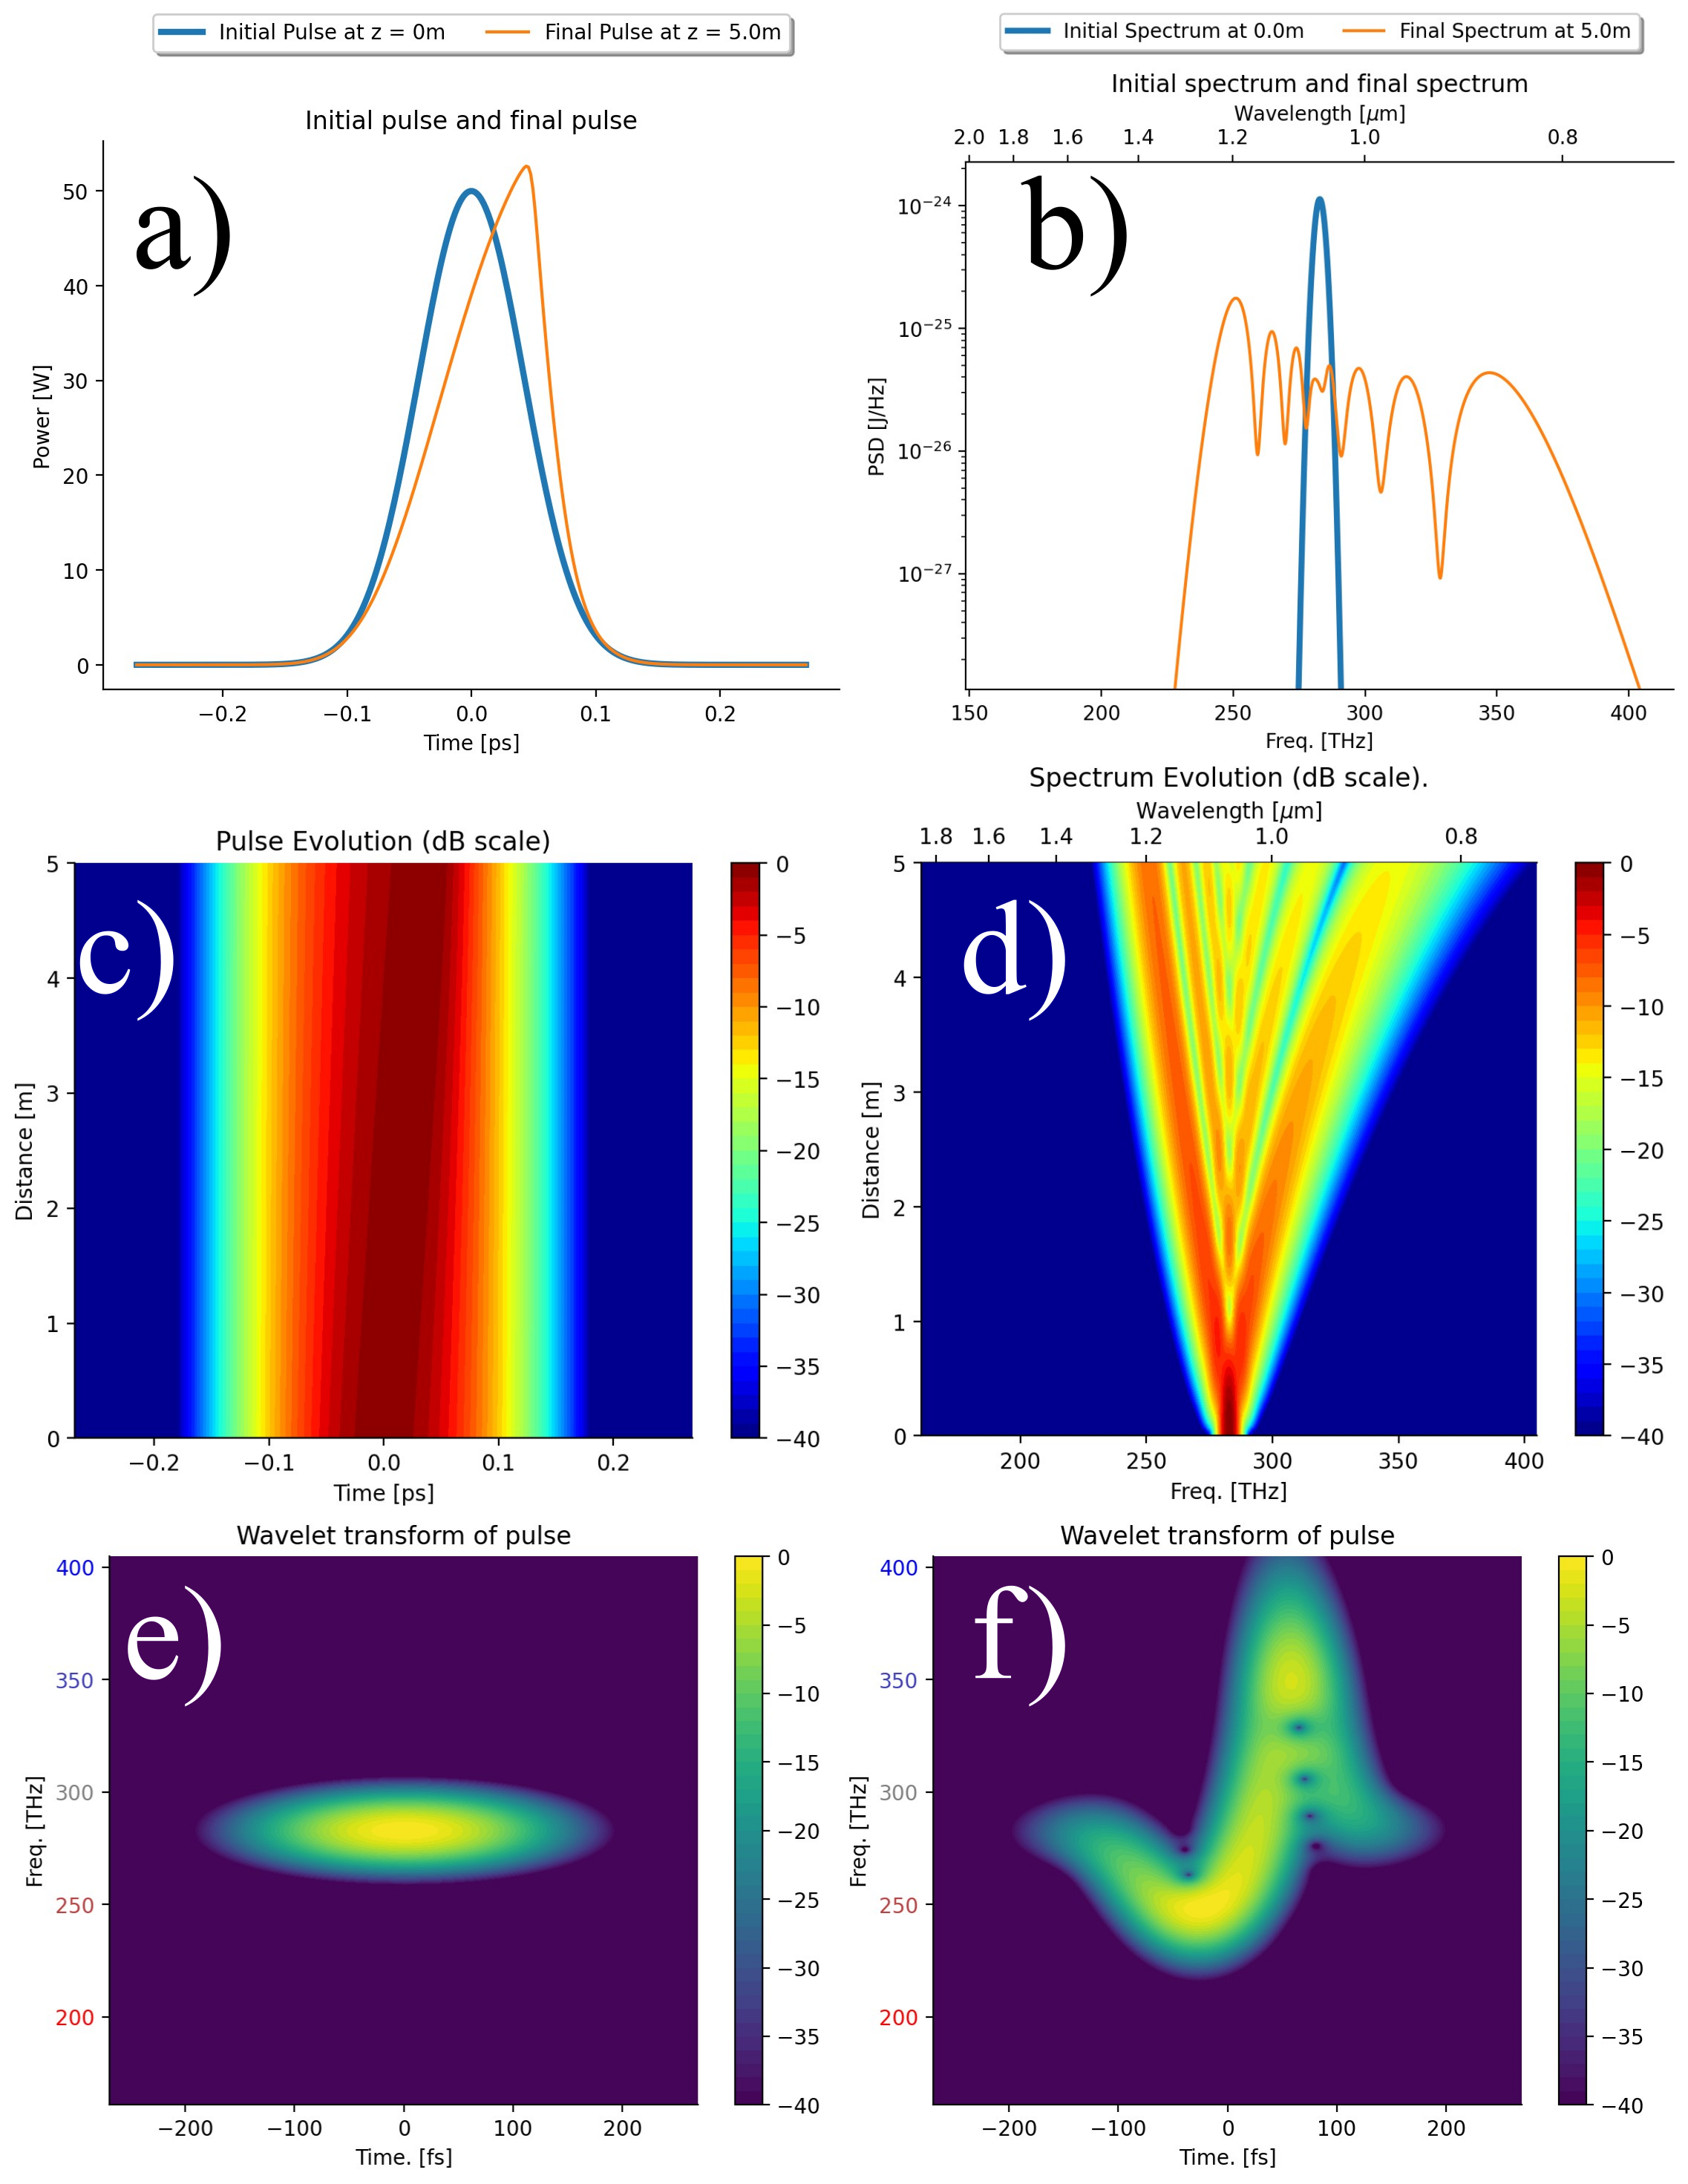
\includegraphics[width=1.0\linewidth]{figures/SPM_and_SS_combined.png}
    \caption{高斯脉冲在由等式~\ref{eq:SS}描述的非线性介质中传播的前后对比。 
    a) 在时域中,脉冲的功率包络在后端变得更陡,因为非线性效应导致脉冲峰值处的折射率较高并减速。 b) 频谱由于后端的陡降坡度向更高频率不对称展宽。 c) 时域中功率包络的演化。 d) 频谱逐渐向高频展宽。 e) 传播前的脉冲频谱图。 f) 传播后的脉冲频谱图。使用\href{https://colab.research.google.com/drive/1P41F4hO6Mv12RsEkpogYv5teQyFZ6iW0?usp=sharing}{这个交互notebook}中的数值模拟生成图形,读者可以尝试进行实验。}
    \label{fig:SS}
\end{figure}

\subsection{适用性}
由于SS的影响与 $\omega_0\approx 2\pi/200~\text{THz} = 2\pi/5$fs 成反比,且对于长脉冲 $\A|\A|^2$ 的时间导数较小,SS效应在脉宽低于100~fs时较为显著,在数百fs量级的脉宽时较为显著,而对于超过几ps的脉宽则可忽略不计。




    \chapter{四波混频}
\label{ch:FWM}

根据公式~\ref{eq:average_power}计算出的单一频率光的平均功率在一段时间内是恒定的。如果存在两个频率,它们之间的干涉会导致平均功率随时间正弦变化。由于 $\gamma\neq0$ 意味着折射率取决于功率,因此在非线性介质中同时存在两个频率的光意味着相位将被正弦调制。这种效应会产生新的频率成分,被称为 “四波混频”(FWM)。



\section{电相位调制}

要了解四波混频,首先要考虑将连续波激光信号发射到商用相位调制器中,并由函数发生器发出的正弦电信号驱动。可视化效果见图 ~\ref{fig:PM},实验演示见 \href{https://youtu.be/j8It3to54AQ}{此视频}。输出端的信号由以下公式给出

\begin{align}
    \label{eq:phase_modulator}
    \E_{out}&=\E_{in}\exp\left(i\Phi\cos(\omega_dT), \right)
\end{align}

其中,$\Phi$ 是调制器传递的最大相移,$\omega_d$ 是调制频率。关于这种调制对 $\E_{out}$ 实部的影响,请参见 \href{https://www.desmos.com/calculator/vcreo1gs2q}{此交互式图表}。使用所谓的 “雅各比-安格尔展开式”~\cite{NIST_JA_expansion},公式~\ref{eq:phase_modulator}中复数指数内的余弦函数可以写为

\begin{align}
\label{eq:JA}
    \exp\left(i\Phi\cos(\omega_dT)\right) &= \sum_{n=-\infty}^{\infty}i^n J_n(\Phi) \exp\left(in\omega_dT\right),
\end{align}
其中,$J_n(\Phi)$ 是$n^{th}$ 阶贝塞尔函数的第 1 种。简而言之,公式 ~\ref{eq:JA} 表明正弦相位调制会产生间隔为 $\omega_d$ 的新的离散频率成分,其相对功率取决于调制幅度 $\Phi$。还请注意,将公式 ~\ref{eq:chirp_definition}应用于公式 ~\ref{eq:phase_modulator}显示,正弦调制会随着时间改变瞬时频率,改变幅度为 $\Phi\omega_d\sin(\omega_dT)$,这进一步表明相位调制会改变入射光的颜色。
\begin{figure}
    \centering
    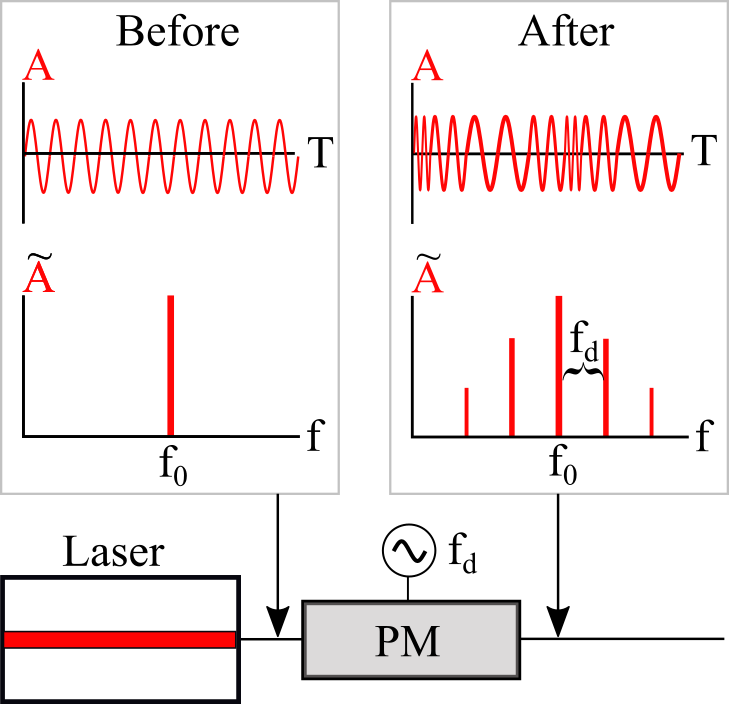
\includegraphics[width=1\linewidth]{figures/PhaseModulator.png}
    \caption{正弦波相位调制对连续波光信号的影响示意图。在进入调制器之前,只有一个激光频率。进入调制器后,根据公式~\ref{eq:JA},光相位在时域中的交替前进和延迟相当于引入了新的频率成分。}
    \label{fig:PM}
\end{figure}

\section{非线性相移}
\label{sec:sidebands}

以下的 FWM 建模方法受到~\cite{Boskovic_Original_Kerr_Effect}中最初提出的方法的启发。考虑公式 ~\ref{eq:SPM_applied},并假设场 $\A(0,T)$ 可以写成两个连续波信号的和,这两个连续波信号的平均功率分别为 $P_a$ 和 $P_b$,频率间隔为 $\Delta\omega$ 。
\begin{align}
    \label{eq:FWM_input}
    \A(0,T)&= \sqrt{P_a}e^{-i\frac{\Delta\omega}{2}T}+\sqrt{P_b}e^{i\frac{\Delta\omega}{2}T}.
\end{align}
当信号由两个持续时间有限的脉冲组成时,连续波假设是一个近似值,当 $\omega_d$ 大于脉冲的带宽时,连续波假设是有效的。非线性介质末端的场为
\begin{align}
    \A(L,T) &= \A(0,T)\exp\left(i\gamma L [P_a+P_b+2\sqrt{P_aP_b}\cos(\omega_dT)] \right) \\ \nonumber
    &= \A(0,T)\exp\left(i\gamma L [P_a+P_b]\right)\exp\left(i2\gamma L\sqrt{P_aP_b}\cos(\omega_dT) \right)\\ \nonumber
    \A(L,T)Q^{-1}&= \A(0,T)\exp\left(i2\gamma L\sqrt{P_aP_b}\cos(\omega_dT) \right)\\ \nonumber
    \A(L,T)Q^{-1}&= \A(0,T)\exp\left(i\phi_{NL}\cos(\omega_dT) \right),
\end{align}
其中,为方便起见,时间无关因子 $Q=\exp(i\gamma L [P_a+P_b])$暂时移至等式左侧。应用公式 ~\ref{eq:JA} 得出
\begin{align}
    \A(L,T)Q^{-1}&= \A(0,T)\sum_{n=-\infty}^{\infty}i^nJ_n(\phi_{NL})e^{in\omega_dT} \\ \nonumber
    &=\left(\sqrt{P_a}e^{-i\frac{\Delta\omega}{2}T}+\sqrt{P_b}e^{i\frac{\Delta\omega}{2}T}\right)\sum_{n=-\infty}^{\infty}i^nJ_n(\phi_{NL})e^{in\omega_dT} \\ \nonumber
    &=\sqrt{P_a}\sum_{m=-\infty}^{\infty}i^mJ_m(\phi_{NL})e^{i\left(m-\frac{1}{2}\right)\omega_dT}+...\\ \nonumber & \quad\quad\quad\quad\quad\sqrt{P_b}\sum_{k=-\infty}^{\infty}i^kJ_k(\phi_{NL})e^{i\left(k+\frac{1}{2}\right)\omega_dT}.
\end{align}

请注意,由于 $\A(0,T)$ 中的两个复指数导致第一个和中 $m=1$ 所对应的频率与第二个和中 $k=1$ 所对应的频率不同,因此最初以 $n$ 为索引的无限和被拆分为两个以 $m$ 和 $k$ 为索引的无限和。要重新组合这两个和,使用 $m=k+1$ 并得到
\begin{align}
\label{eq:re_index}
    \A(L,T)Q^{-1}&=\sqrt{P_a}\sum_{k=-\infty}^{\infty}i^{k+1}J_{k+1}(\phi_{NL})e^{i\left(k+\frac{1}{2}\right)\omega_dT}+...\\ \nonumber & \quad\quad\quad\quad\quad\sqrt{P_b}\sum_{k=-\infty}^{\infty}i^kJ_k(\phi_{NL})e^{i\left(k+\frac{1}{2}\right)\omega_dT} \\ \nonumber
    &= \sum_{n=-\infty}^{\infty} i^n\left[i\sqrt{P_a}J_{n+1}\left(\phi_{NL}\right)+\sqrt{P_b}J_n\left(\phi_{NL}\right)\right]e^{i\omega_d\left(n+\frac{1}{2}\right)T}.
\end{align}
最后,把 $Q$ 移到公式 ~\ref{eq:re_index} 的右边,得到
\begin{align}
\label{eq:FWM_general}
    \A(L,T)&=\sum_{n=-\infty}^{\infty} i^n\left[i\sqrt{P_a}J_{n+1}\left(2\gamma L\sqrt{P_aP_b}\right)+\sqrt{P_b}J_n\left(2\gamma L\sqrt{P_aP_b}\right)\right]e^{i\omega_d\left(n+\frac{1}{2}\right)T+i\gamma L[P_a+P_b]}.
\end{align}

在公式 ~\ref{eq:FWM_general}中,$n=-1$ 的频率分量将位于 $-\omega_d/2$,而 $n=0$ 的频率分量将位于 $+\omega_d/2$,与公式 ~\ref{eq:FWM_input}中的原始两个频率相对应。$n^{th}$ 阶边带的平均功率为
\begin{align}
\label{eq:sideband_power}
    |\A_n(L,T)|^2 &= P_aJ^2_{n+1}\left(2\gamma L \sqrt{P_aP_b}\right)+P_bJ^2_{n}\left(2\gamma L \sqrt{P_aP_b}\right).
\end{align}
请参见图(fig:FWM)a) 和 b),这是针对不同的 $2\gamma L \sqrt{P_aP_b}$ 值对边带功率进行的数值模拟。请参见图 ~\ref{fig:FWM} c) ,比较数值计算的边带功率和公式 ~\ref{eq:sideband_power}预测的功率。假设 $P_a\ll P_b$ 和 $2\gamma L\sqrt{P_aP_b}<\sqrt{1+n}$ 且 $n>0$ 可以得到

\begin{align}
\label{eq:sideband_approx}
    |\A_n(L,T)|^2 &\approx P_b\frac{(\gamma^2 L^2P_aP_b)^{n}}{n!^2},
\end{align}
since
\begin{align}
\label{eq:Bessel_approx}
    J_n(x)&\approx \frac{1}{n!}\left(\frac{x}{2}\right)^n
\end{align}

为贝塞尔函数中的参数。请参见图~ref{fig:FWM} d) 以了解公式~\ref{eq:sideband_approx}预测的缩放行为。与低阶边带相比,高阶边带的功率对输入功率的变化更为敏感,这一事实对于各种全光信号处理技术非常有用~\cite{my_thesis,BenoitPhD,YangLuPhD}。请参阅(\href{https://youtu.be/0SXPvO89jto}{本教程视频},了解将色散因素考虑在内的全波调制建模的不同方法。参见 \href{https://youtu.be/gsa9hrCbnqI}{这段视频},了解四波混频的实验演示。
\begin{figure}
    \centering
    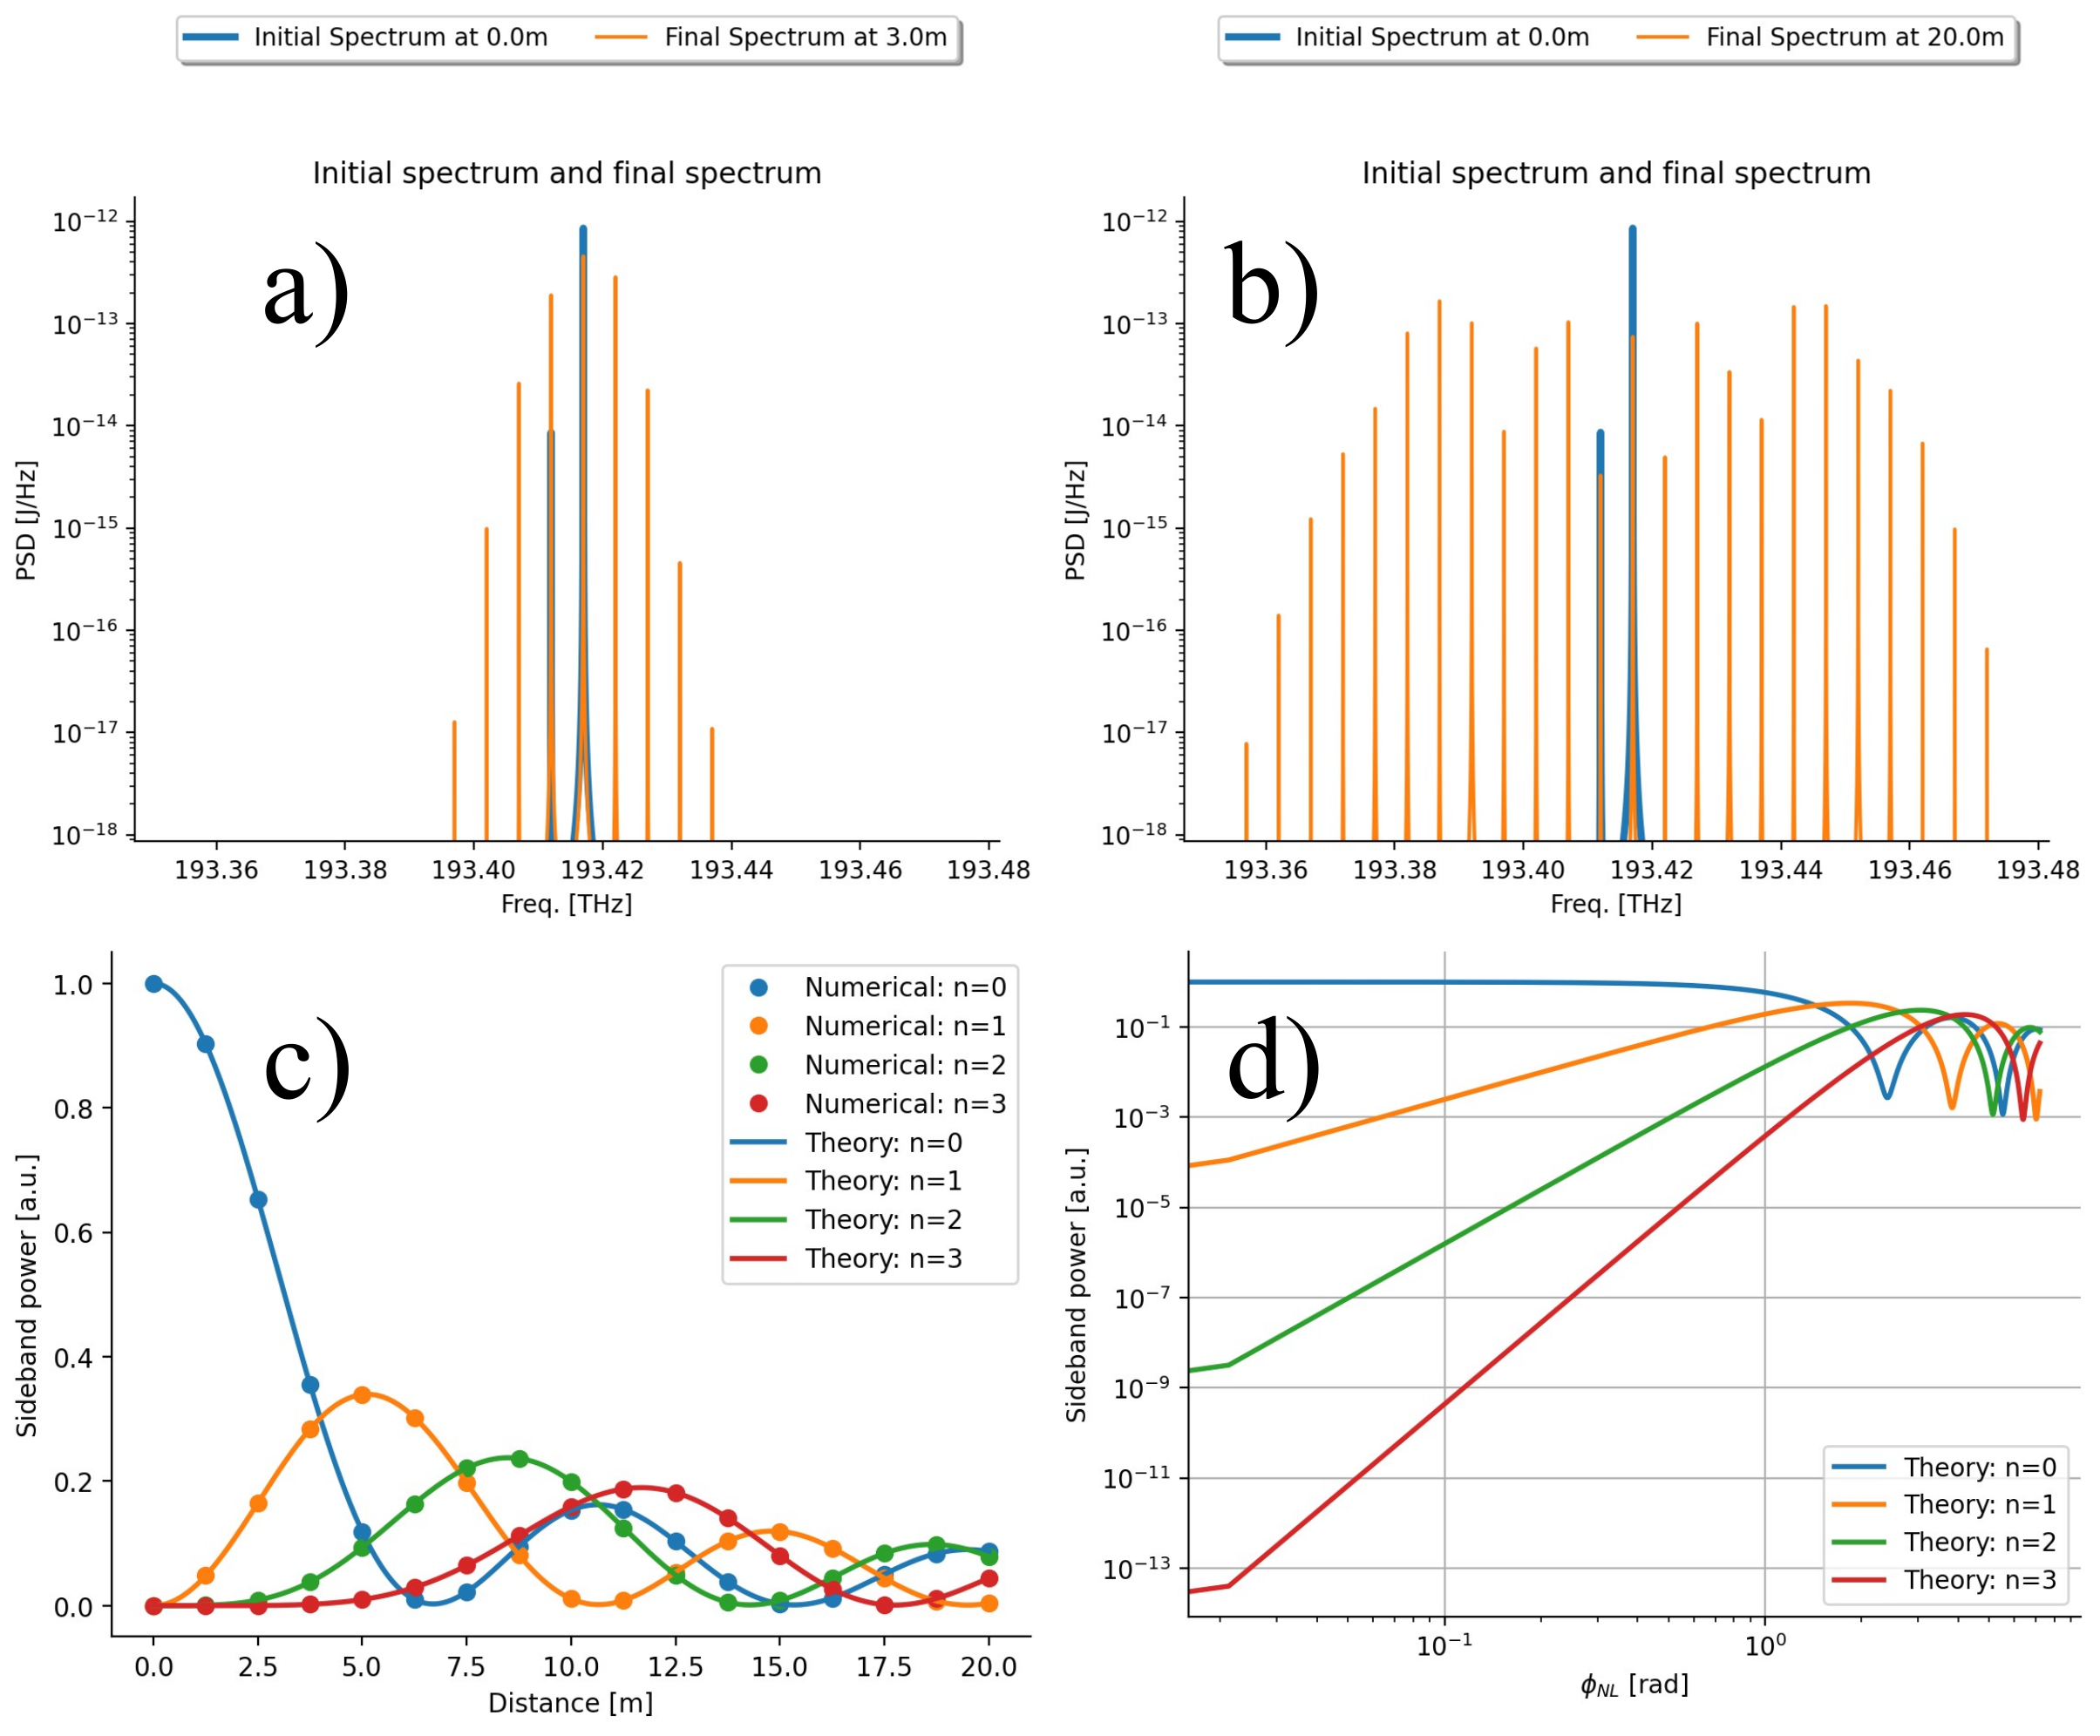
\includegraphics[width=1.0\linewidth]{figures/FWM_combined.png}
    \caption{a) 当两个相距 5~GHz 的频率($P_b=100P_a$)在介质中传播时,数值计算的初始和最终频谱,其中 $\phi_{NL}=2\gamma L\sqrt{P_aP_b}=1.08$~rad. b) 与 a) 相同,但 $\phi_{NL}=2\gamma L\sqrt{P_aP_b}=7.2$~rad. c) 根据数值模拟和公式~\ref{eq:sideband_power},边带功率归一化为 $P_b$ 的比较。 d) 与 c) 类似,但绘制了双对数刻度与 $\phi_{NL}$ 的关系图,以展示公式~\ref{eq:sideband_approx}预测的缩放行为。这些图是使用 \href{https://colab.research.google.com/drive/1l054EDg-50aK5GORN_md4_-tlFy4jwC5?usp=sharing}{这个交互式笔记本}生成的,我们鼓励读者尝试使用。   }
    \label{fig:FWM}
\end{figure} 

\section{交叉相位调制(XPM)}
\label{Sec:XPM}
第~\ref{ch:SPM}章指出,非线性介质中单频光场的相位与该场的平均功率呈线性增长。当存在两个频率时,一个频率分量的相位与其自身的平均功率和另一个频率分量的平均功率的函数关系可以通过公式~\ref{eq:FWM_general}计算出来。选择 $n=0$ 分量可得到
\begin{align}
    \phi_0 &= \frac{\omega_d}{2}T+\gamma L [P_a+P_b]+\theta_0,
\end{align}
这里,
\begin{align}
\label{eq:theta}
    \theta_0 &= arg\left( i\sqrt{P_a}J_{1}\left(2\gamma L\sqrt{P_aP_b}\right)+\sqrt{P_b}J_0\left(2\gamma L\sqrt{P_aP_b}\right) \right) \\ \nonumber
    &= \arctan\left(\frac{\sqrt{P_a}J_{1}\left(2\gamma L\sqrt{P_aP_b}\right)}{\sqrt{P_b}J_0\left(2\gamma L\sqrt{P_aP_b}\right) } \right).
\end{align}
使用公式~\ref{eq:Bessel_approx}可以将公式~\ref{eq:theta}写成
\begin{align}
    \theta_0 &\approx\arctan\left(\frac{\sqrt{P_a}\gamma L\sqrt{P_aP_b}}{\sqrt{P_b} } \right) \\ \nonumber
    &\approx\arctan\left(\gamma LP_a\right) \\ \nonumber
    &\approx \gamma LP_a.
\end{align}
因此,$n=0$ 频率分量的相位为
\begin{align}
    \label{eq:XPM}
    \phi_0 &\approx \frac{\omega_d}{2}T+\gamma L [P_a+P_b]+\gamma LP_a \\ \nonumber
    &=\frac{\omega_d}{2}T+\gamma L [2P_a+P_b].
\end{align}
请注意,$n=0$ 为 $+\omega_d/2$ 处的频率,该频率最初的平均功率为 $P_b$。因此,式 ~\ref{eq:XPM} 中包含 $P_b$ 的项对应于 SPM 的影响,而包含 $P_a$ 的项对应于所谓的 “交叉相位调制”(XPM)。有趣的是,公式 ~\ref{eq:XPM} 显示 XPM 是 SPM 的 “两倍强”,如图 ~\ref{fig:XPM} 所示。参见 \href{https://youtu.be/aDXd13zLPC4}{本视频教程},从麦克斯韦方程出发,对 XPM 的影响进行了另一种推导。请参见 \href{https://www.desmos.com/calculator/vstlwgtlyb}{此交互式图表},以说明 SPM 和 XPM 对两个不同频率的波的相对影响。
\begin{figure}
    \centering
    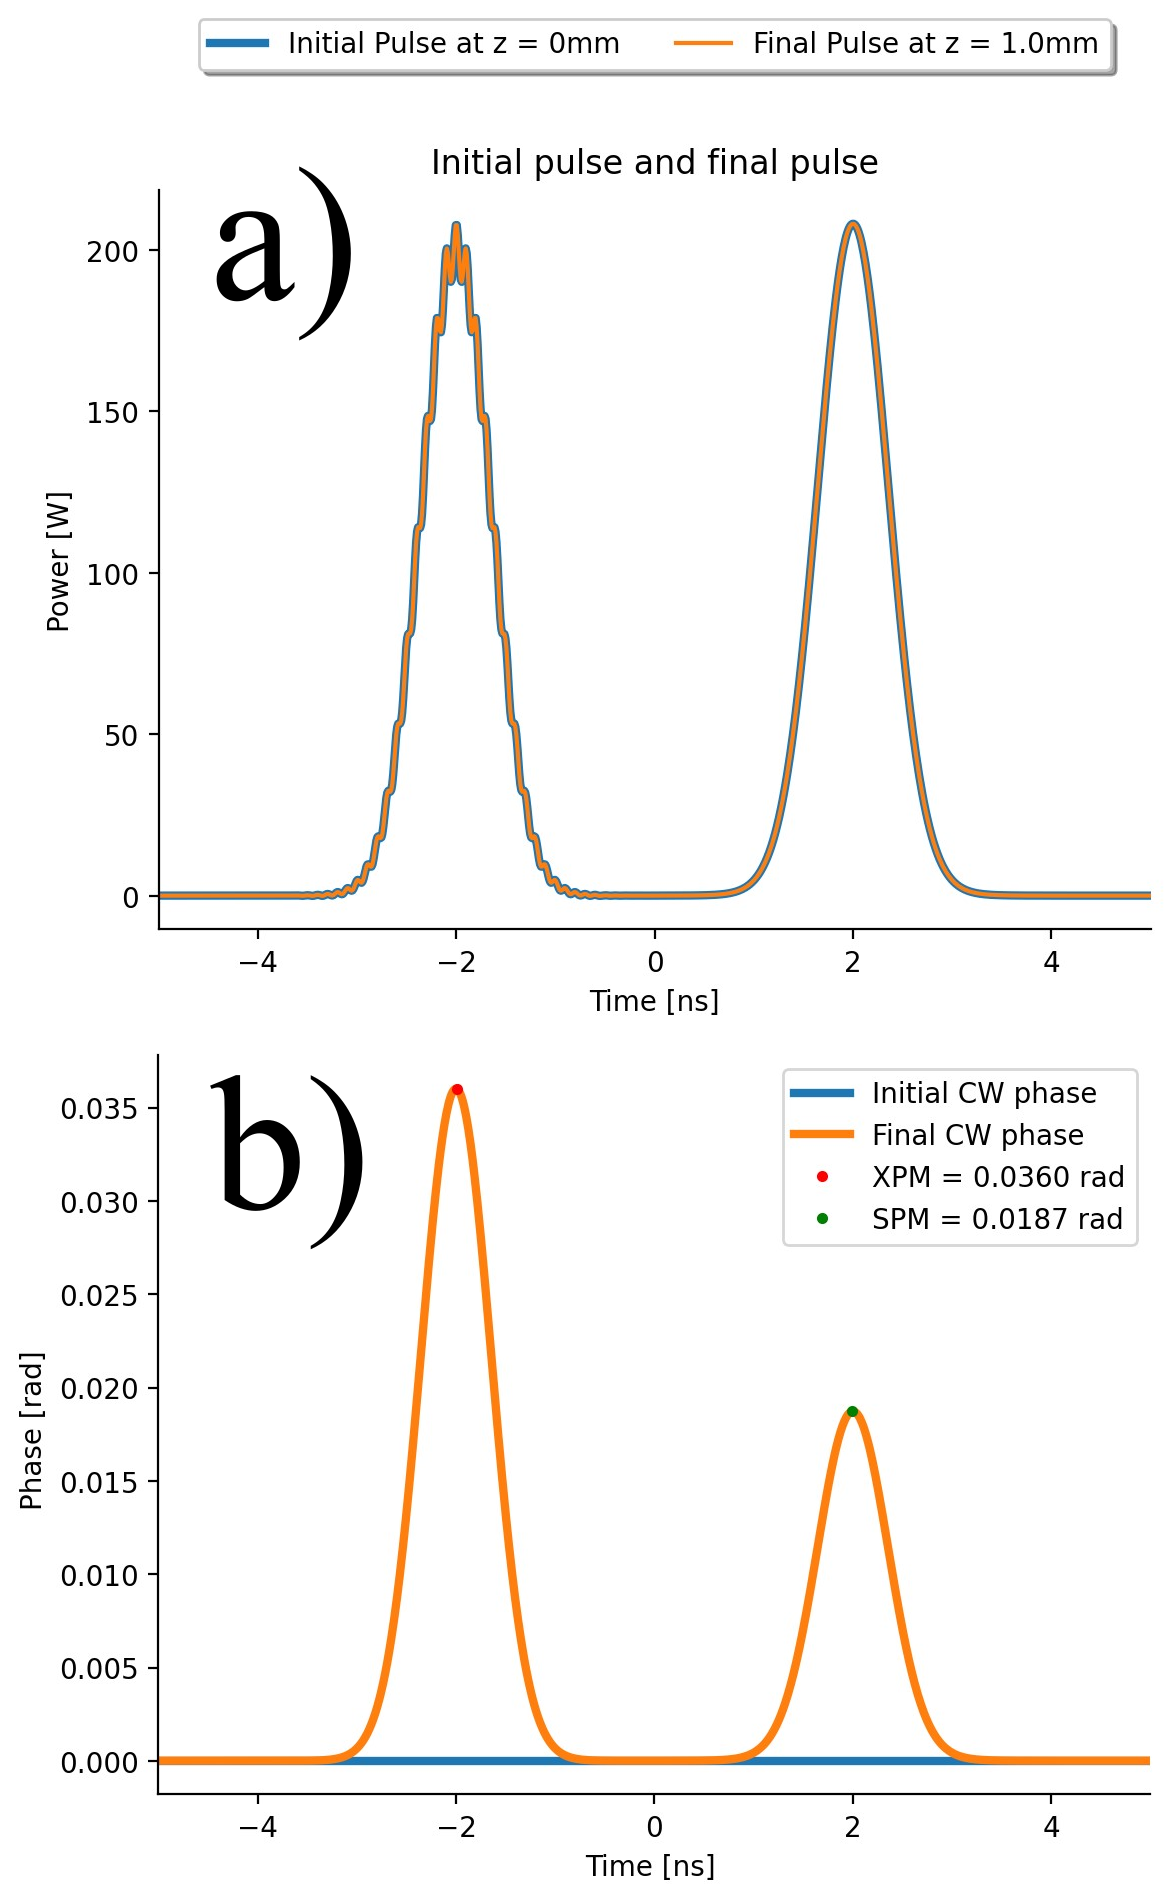
\includegraphics[width=0.8\linewidth]{figures/XPM_combined.png}
    \caption{图示 SPM 和 XPM 对光信号相位的不同影响。 a) 低功率 CW 信号与两个相同的高功率高斯脉冲重叠的时域表示,这两个脉冲的载波频率仅有差别。左侧脉冲的载波频率比 CW 光的载波频率低 10~GHz。 b) 模拟在非线性介质中的传播后,CW 光从 XPM 得到的相移大约是 SPM 的两倍,正如公式 ~\ref{eq:XPM} 所预测的那样。$0.0360/0.0187\approx 1.925\neq2$的比率归因于公式 ~\ref{eq:XPM} 中涉及的近似值以及模拟的有限时间分辨率。这些数字是使用 \href{https://colab.research.google.com/drive/1aIRradfOZGN7JYUhbtYJdVzJwAZoYoUe?usp=sharing}{这个交互式笔记本}生成的,我们鼓励读者尝试使用。}
    \label{fig:XPM}
\end{figure}






\section{相位匹配}
\label{sec:Phase_matching}
小节~\ref{subsec:sidebands}中的推导假定色散可以忽略不计,这是小$\omega_d$值和载波频率接近小节~\ref{subsec:ZDF}中解释的零色散频率的情况。在 \href{https://youtu.be/0SXPvO89jto}{本视频教程}中解释了色散对全波调制的影响。事实证明,当 $\betag_2$ 为正值时,FWM 很弱,而当 $\betag_2$ 为负值时,FWM 最为显著。
\begin{align}
\label{eq:phase_matching}
0&=\betag_2\omega_d^2+\gamma(P_a+P_b)    \\ \nonumber
\betag_2&=-\gamma(P_a+P_b)/\omega_d^2<0,    
\end{align}
假设 $\omega_d$ 足够小,使得在方程~\ref{eq:beta_approx} 中 $\beta_2$ 是唯一相关的项。其原因在于,四波混频(FWM)作为一种过程,涉及电磁波之间通过非线性介质的折射率变化进行**相干**的能量传递。简单来说,非线性效应确保了入射电磁波会引起介质中构成微小偶极子的振荡,从而产生新的时间频率。如果这些偶极子振荡的某一时间频率对应的空间频率与另一电磁波的空间频率相同,该电磁波的功率将通过相干叠加随着传播距离增加而增大,如 \href{https://youtu.be/bha8SzWzRc4}{此视频教程} 所解释的那样。

方程~\ref{eq:phase_matching} 的要求源于入射波与新产生波的空间频率差需要很小,同时入射场功率引起的折射率增大使得空间频率比正常情况更大。因此需要负值的 $\beta_2$ 来进行补偿。这种现象,即介质正常折射率引起的空间频率变化与场功率通过非线性引起的空间频率变化达到平衡,被称为“相位匹配”。方程~\ref{eq:phase_matching} 中的相位匹配条件专门针对四波混频的特殊情况,而类似的表达式也可以推导出适用于本教程范围之外的其他非线性效应,例如 \href{https://www.youtube.com/watch?v=UpuN0dS23Nw}{二次谐波生成}、\href{https://youtu.be/bha8SzWzRc4}{三次谐波生成} 以及 \href{https://www.creol.ucf.edu/mir/wp-content/uploads/sites/7/2023/07/L22_-Stimulated-Brillouin-scattering.pdf}{受激布里渊散射}。
\subsection{调制不稳定(MI)}
由于四波混频(FWM)的影响,在某种非线性介质中,如果载波频率对应的 $\beta_2<0$,信号在传播过程中会变得更加噪声化。这是因为载波与电磁场中微小且无处不在的波动之间的干涉会引发 FWM,将光功率从载波转移到相邻频率上,如 \href{https://prefetch.eu/know/concept/modulational-instability/}{此处} 所解释,并在图~\ref{fig:MI} 中进行了说明。这种由相位匹配导致特定噪声频率被优先放大的过程被称为“调制不稳定性”(Modulation Instability, MI)。关于 MI 的更多细节,请参见 \href{https://youtu.be/VtaoPd0Fwj8}{此视频教程}。

\begin{figure}
    \centering
    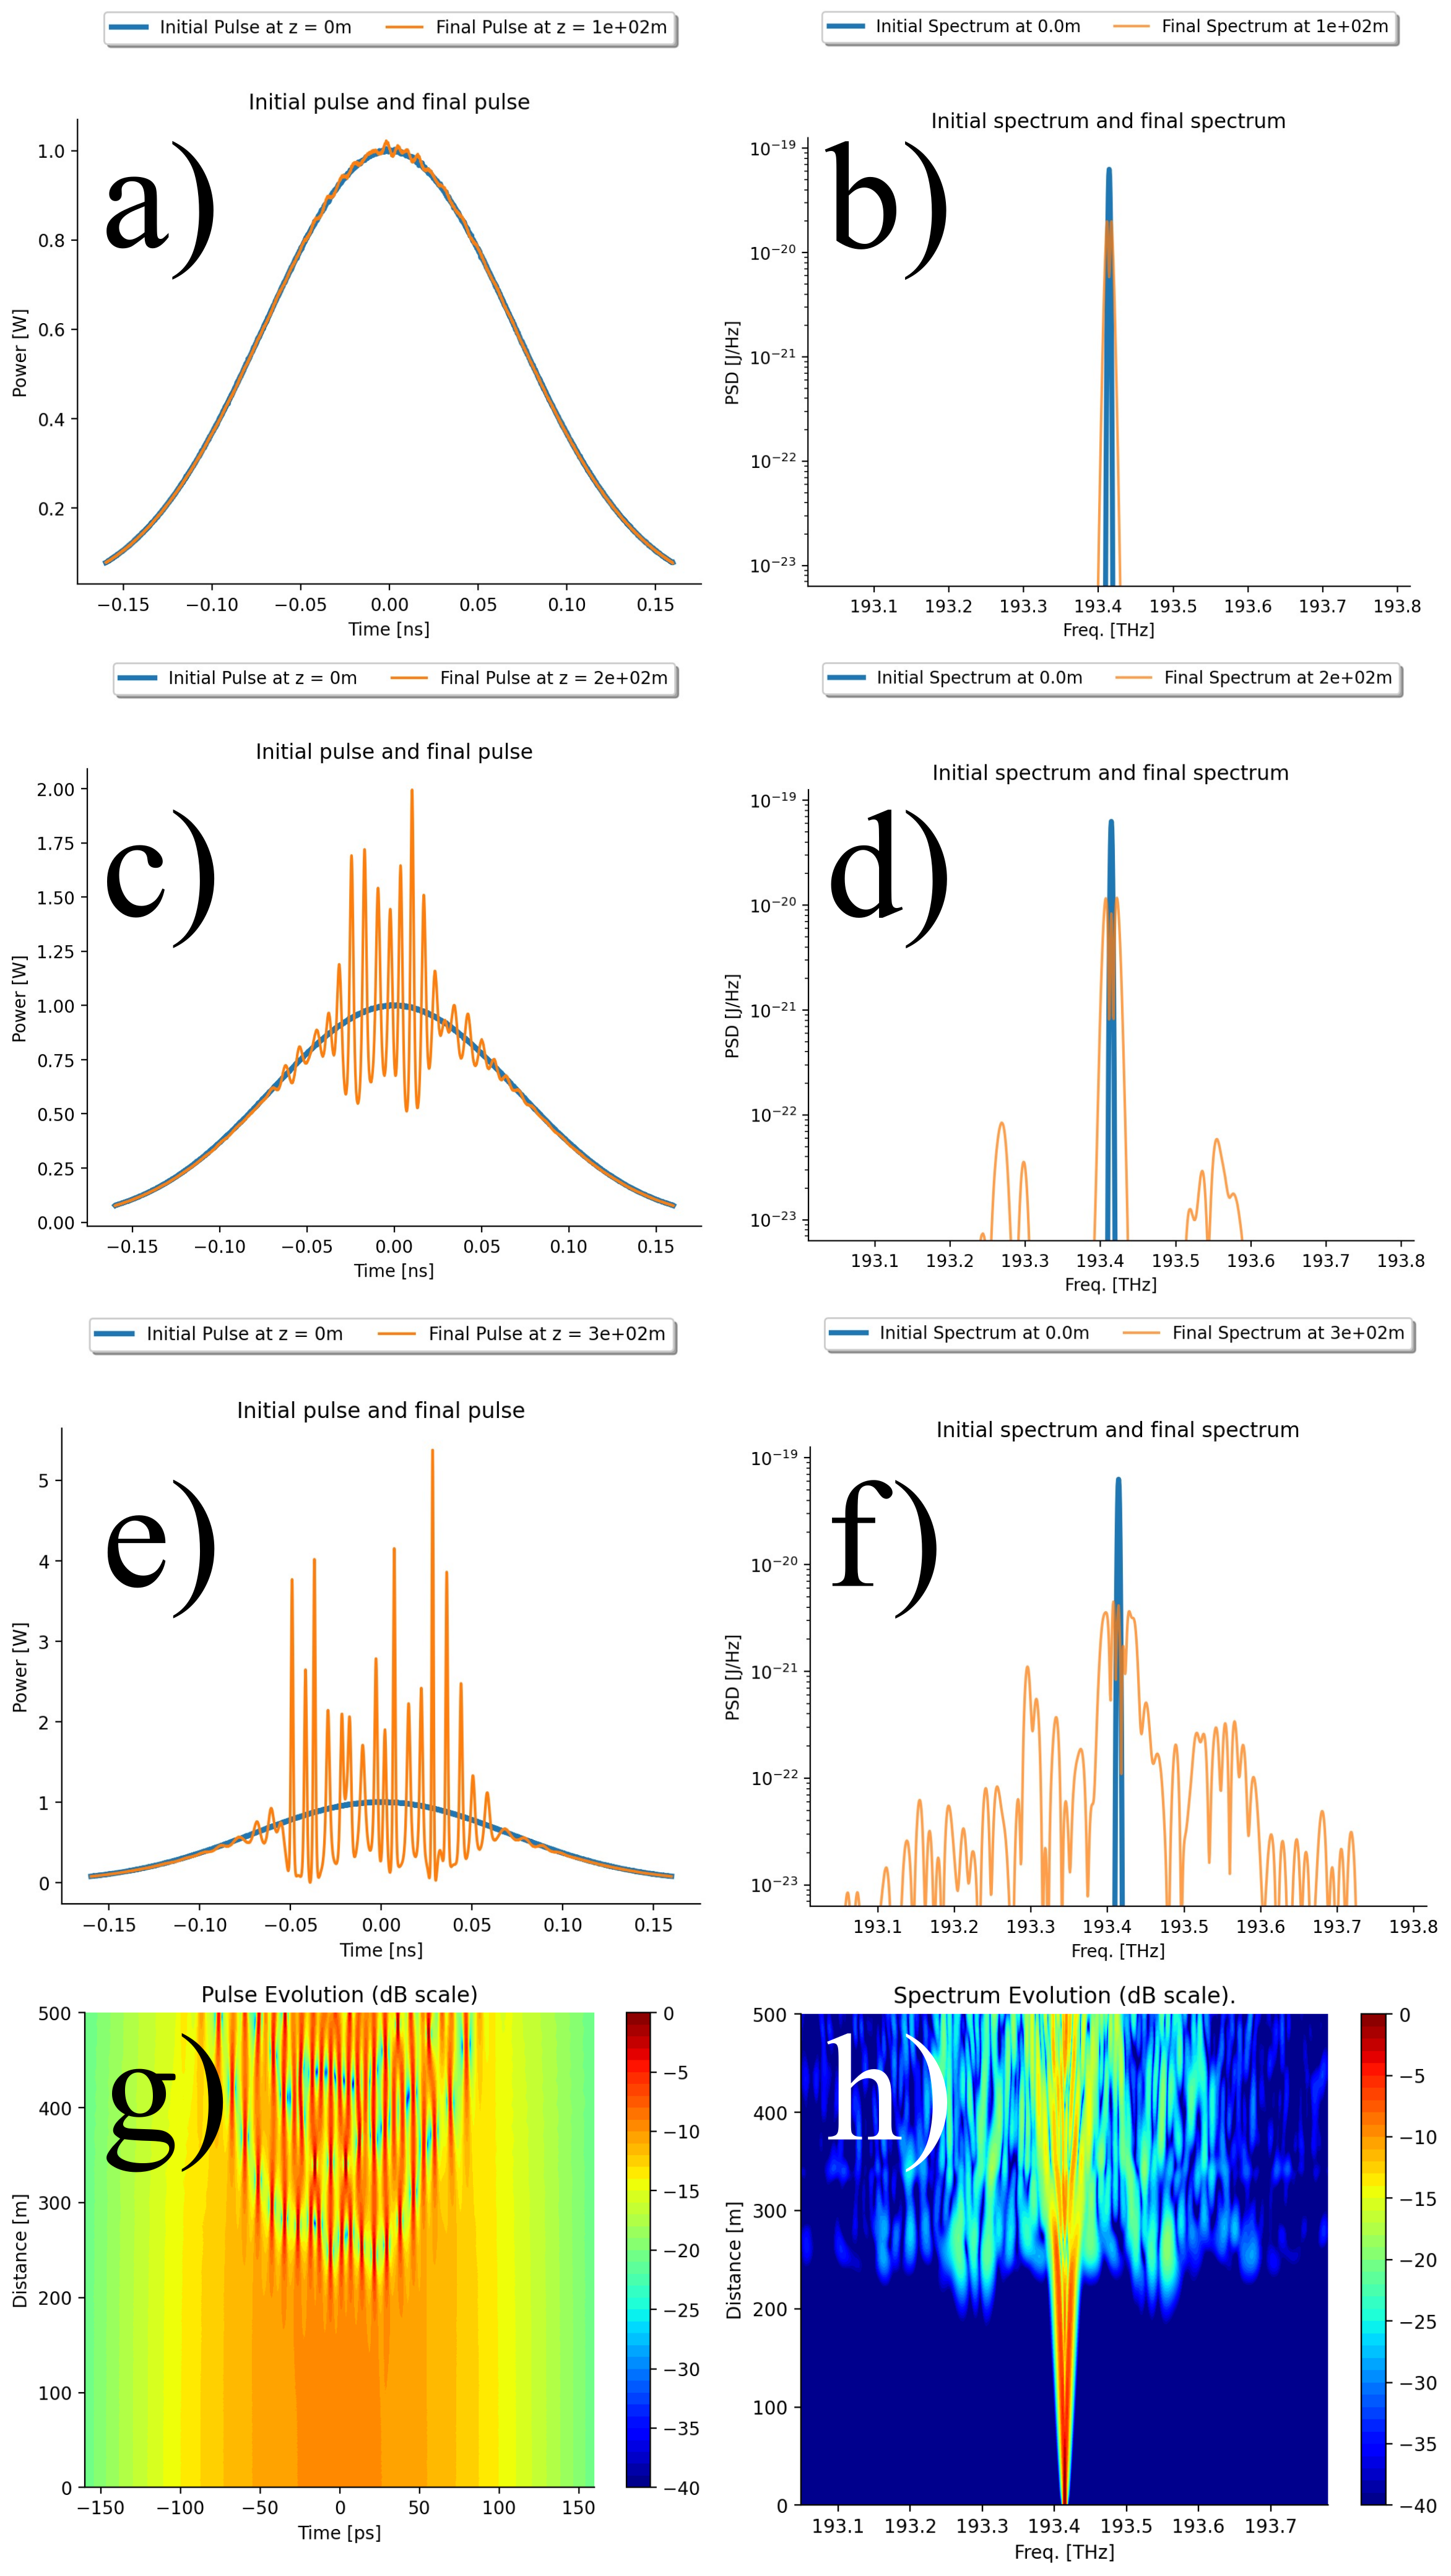
\includegraphics[width=0.75\linewidth]{figures/MI_combined.png}
    \caption{a) 初始和最终时间域信号功率:信号由高斯脉冲和幅度比高斯脉冲小 1.000 倍的随机噪声组成,通过具有 $\beta_2<0$ 的非线性介质传播 100m 后的情况。b) 与 a) 相同,但展示频谱。c-d) 与 a-b) 相同,但传播距离为 200m。e-f) 与 a-b) 相同,但传播距离为 300m。g) 信号在传播 500m 内的完整时间演化。h) 与 g) 相同,但展示频谱。图像由 \href{https://colab.research.google.com/drive/1p2aQZ4zPPAIMplVxvlezdmpQt_j-rsY7?usp=sharing}{此交互式笔记本} 生成,读者可以尝试使用该笔记本进行实验。}
    \label{fig:MI}
\end{figure}




    \chapter{拉曼效应}
\label{ch:Raman}

当暴露在振荡电磁场中时,介质中的电子由于质量较小,几乎会立即做出反应。而这些电子绕其运行的原子核由于质量相对较大,反应速度要慢得多。因此,影响某一光纤段脉冲特定瞬间的非线性相移取决于两点: 该瞬间脉冲的光功率和过去影响该位置的光功率。材料晶格中原子核的延时机械振动对电磁场的非线性影响被称为 “拉曼效应”~\cite{Raman_original}。 


\section{拉曼响应函数}
在数学上,拉曼效应对光脉冲的影响可以用以下公式描述
\begin{align}
\label{eq:raman}
 \partial_z \A = i\gamma\left( 
\A \int_{0}^{\infty} R(T_{delay})|\A(z,T-T_{delay})|^2 dT_{delay} \right),
\end{align}
在忽略损耗、色散和自陡的情况下,它等价于公式 ~\ref{eq:GNLSE}。函数 $R(T_{delay})$ 是总响应函数,表示过去不同时间的功率对给定瞬间影响脉冲的非线性相移的贡献程度。它可以通过三角函数写成电子响应的瞬时贡献与晶格振动引起的延迟拉曼响应之和,即
\begin{align}
    \label{eq:response}
    R(T_{delay})&= (1-f_R)\delta(T_{delay})+f_Rh_R(T_{delay}),
\end{align}
其中,$0\leq f_R\leq 1$ 是一个标量,决定了两个贡献的相对大小。拉曼响应函数的确切函数形式 $h_R(T_{delay})$ 取决于材料,但通常类似于一个乘以阻尼项的正弦函数,并且必须满足 $\int_{-\infty}^{\infty}h_R(T_{delay}) dT_{delay}=1$,因为它本质上是 “权衡 ”过去不同时间的功率对当前非线性相移的贡献程度。 此外,必须要求 $h_R(T_{delay})=0$ for $T_{delay}\leq0$ 以防止该表达式违反因果关系,让 \emph{future} 功率影响当前的非线性相移。请参阅 \href{https://www.desmos.com/calculator/bdg6icprch}{此交互图},了解过去的功率对拉曼效应引起的相移的影响。
直观地说,函数 $h_R(T_{delay})$就像描述音叉、钢琴键或吉他弦突然被敲击后声波振幅的函数一样,是一种逐渐 “回落 ”的振荡。继续类比,如果把 $|\A(z,T-T_{delay})|^2$ 看作是在不同时间具有不同强度的瞬时击打的大集合,那么当前的振荡取决于过去的所有振荡就说得通了。 
将公式 ~\ref{eq:response}代入公式 ~\ref{eq:raman},并对三角函数进行积分求得
\begin{align}
    \label{eq:raman_split}
    \partial_z \A = i\gamma\A\left( 
(1-f_R)|\A(z,T)|^2+f_R \int_{0}^{\infty} h_R(T_{delay})|\A(z,T-T_{delay})|^2 dT_{delay} \right).
\end{align}
请注意,如果脉冲功率的变化与响应函数的持续时间相比非常缓慢,则可以近似地计算 $h_R(T_{delay})\approx \delta(T_{delay})$(或者,等价地计算 $|\A(z,T-T_{delay})|^2\approx|\A(z,T)|^2$),在这种情况下,公式~\ref{eq:SPM}就恢复了。换句话说,只有当脉冲持续时间接近分子晶格自然振荡的持续时间时,拉曼效应才会明显!假设脉冲持续时间明显长于 $h_R(T_{delay})$的持续时间,因此不同时间延迟下的功率可以通过将当前功率及其梯度线性外推到过去来找到,那么公式~\ref{eq:raman_split}中的积分可以写为 
\begin{align}
\label{eq:raman_approx}
    f_R \int_{0}^{\infty} h_R(T_{delay})|\A(z,T-T_{delay})|^2 dT_{delay} &\approx\\ \nonumber \quad\quad\quad f_R \int_{0}^{\infty} h_R(T_{delay})\left[ 
  |\A(z,T)|^2-T_{delay}\partial_T|\A(z,T)|^2 \right] dT_{delay} &=\\ \nonumber \quad\quad\quad  |\A(z,T)|^2f_R- \partial_T|\A(z,T)|^2 f_R\int_{0}^{\infty} T_{delay} h_R(T_{delay}) 
   dT_{delay}&=\\ \nonumber \quad\quad\quad  |\A(z,T)|^2f_R- \partial_T|\A(z,T)|^2 T_R &,
\end{align}
其中 $T_R$ 是拉曼响应函数的平均持续时间,用 $f_R$ 缩放。将公式~\ref{eq:raman_approx}的结果代入公式~\ref{eq:raman_split}可得
\begin{align}
    \label{eq:raman_approx_applied}
\partial_z \A = i\gamma\A\left( 
|\A(z,T)|^2-T_R \partial_T|\A(z,T)|^2\right),
\end{align}
其中包含与电流功率成比例的 “常规 ”SPM 项,以及取决于功率时间导数的附加项。对于二氧化硅,$T_R/approx 3$~fs,因此公式 ~\ref{eq:raman_approx_applied}将对超过约 600~fs 的脉冲有效。公式 ~\ref{eq:raman_approx}中应用的近似值可以扩展到包括 $|\A(z,T)|^2$ 的二阶导数,以提高精确度。从公式 ~\ref{eq:SPM_example} 和 Fig.~\ref{fig:chirp_profiles} 中回想一下,“常数 ”SPM 项会导致瞬时频率大幅下降,而此时功率的 \emph{derivative} 值非常正(原文如此)。根据同样的逻辑,公式 ~\ref{eq:raman_approx_applied}中的拉曼项会导致 “导数的导数 ”为负的瞬时频率大幅下降。换句话说,拉曼效应会在脉冲峰值处产生红移,而在其他地方不会产生等效的大蓝移,从而使整个脉冲 “更红”!从物理学角度来看,红移的产生是因为入射光子会激发介质晶格的机械振动,从而损失部分能量。
\subsection{$h_R(T_{delay})$的表达式}
假设分子振动以单一频率为主,二氧化硅中拉曼效应的近似表达式为 
\begin{align}
\label{eq:raman_basic}
    h_R^{basic}(T_{delay})&= \left(\frac{1}{\tau_1^{2}}+\frac{1}{\tau_2^{2}} \right)\tau_1\exp\left(-\frac{T_{delay}}{\tau_2}\right)\sin\left(\frac{T_{delay}}{\tau_1}\right),
\end{align}
其中 $f_R=0.18$,$\tau_1=12.2$~fs,$\tau_2=32$~fs。为了尊重因果关系,所有列出的 $h_R(T_{delay})$表达式都假定 $T_{delay}\leq0$ 为零。在数学上,这可以通过乘以 Heaviside 阶跃函数来确保。对于二氧化硅的振动行为,比公式 ~\ref{eq:raman_basic} 更精确的近似值是  
\begin{align}
\label{eq:raman_new}
    h_R^{better}(T_{delay})&= (1-f_b) h_R^{basic}(T_{delay})+f_b\frac{2\tau_b-T_{delay}}{\tau_b^2}\exp\left(-\frac{T_{delay}}{\tau_b}\right),
\end{align}
其中,$f_R=0.245$,$f_b=0.21$,$\tau_b=96$~fs。二氧化硅拉曼响应的精确表达式为
\begin{align}
\label{eq:Raman_exact}
    h_R^{exact}(T_{delay})&=c^{-1}_{norm}\sum_{n=0}^{12}C_n\exp\left(- g_nT_{delay}-0.25G_n^2T^2_{delay}  \right)\sin\left(2\pi \nu_nT_{delay} \right),
\end{align}
其中,$f_R=0.18$,参数$C_n$、$g_n$、$G_n$和$\nu_n$列于表 ~\ref{tab:raman_coeffs},$c_{norm}=3.75225$~ps,因此$\int_0^\infty h_R^{exact}(T_{delay}) dT_{delay}=1$。图 ~\ref{fig:raman_combined}展示了这三种二氧化硅拉曼响应模型的可视化及其对同一光脉冲的影响。图 ~\ref{fig:raman_combined}~b) 中绘制了 $h_R(T_{delay})$ 不同表达式的傅立叶变换虚部。从物理角度看,这些光谱意味着拉曼效应允许特定光学频率从其上方 13~THz 的频率 “窃取 ”功率,并迫使其向下方 13~THz 的频率 “捐赠 ”功率。由于与章节 ~\ref{sec:KK_relations}中所述的原因类似,光谱的实部(未显示)与拉曼效应引起的折射率变化有关,因此可以确定其引起的时间延迟。根据图 ~\ref{fig:raman_combined}~b) 中所示曲线的最大值,最大拉曼增益以及拉曼效应变得显著的特征长度可以表示为
\begin{align}
    g_{Raman} &= \frac{4}{3} \gamma f_R P_0 n(\omega_0)\cdot \text{max}( \text{Im} \{ \FT \{ h_R(T_{delay}) \}(\omega) \} )\\ 
    L_{Raman} &= \frac{1}{g_{Raman}},
\end{align}
其中,$P_0$ 是脉冲的最大功率,$n(\omega_0)$ 是介质的折射率(对于二氧化硅,折射率约为 $1.47$)。有关拉曼效应的更多信息,请参见 \href{https://www.youtube.com/playlist?list=PLdFybGSAoPnn6tnSmptR71zKAgcKsjIfi}{这些视频教程}。  
\begin{table}
\begin{center}
    \begin{tabular}{c|c|c|c|c}
    \label{tab:raman_coeffs}
        n  &$C_n$ & $g_n$ [fs] & $G_n$ [fs] & $\nu_n$ [THz]  \\ \hline
        0  &  1    &0.521       &1.562          &1.69   \\
        1  &  11.4 &1.163       &3.310          &3.00   \\
        2  &  36.67&1.749       &5.246          &6.93   \\
        3  &  67.67&1.624       &4.872          &10.87\\
        4  &  74   &1.352       &4.057          &13.88       \\
        5  &  4.5  &0.245       &0.734          & 14.90   \\
        6  &  6.8  &0.415       &1.244          & 18.33   \\
        7  &  4.6  &1.549       &4.647          & 20.74   \\
        8  &  4.2  &0.594       &1.784          & 23.79  \\
        9  &  4.5  &0.642       &1.928          & 25.05   \\
        10 &  2.7  &1.499       &4.497          & 27.88   \\
        11 &  3.1  &0.909       &2.728          & 32.38   \\
        12 &  3    &1.599       &4.797          &   36.42 
    \end{tabular}
    \caption{公式~\ref{eq:Raman_exact}中二氧化硅拉曼响应精确表达式的参数表,由 \cite{raman_exact}修改而来。  }
    \end{center}
\end{table}

\begin{figure}
    \centering
    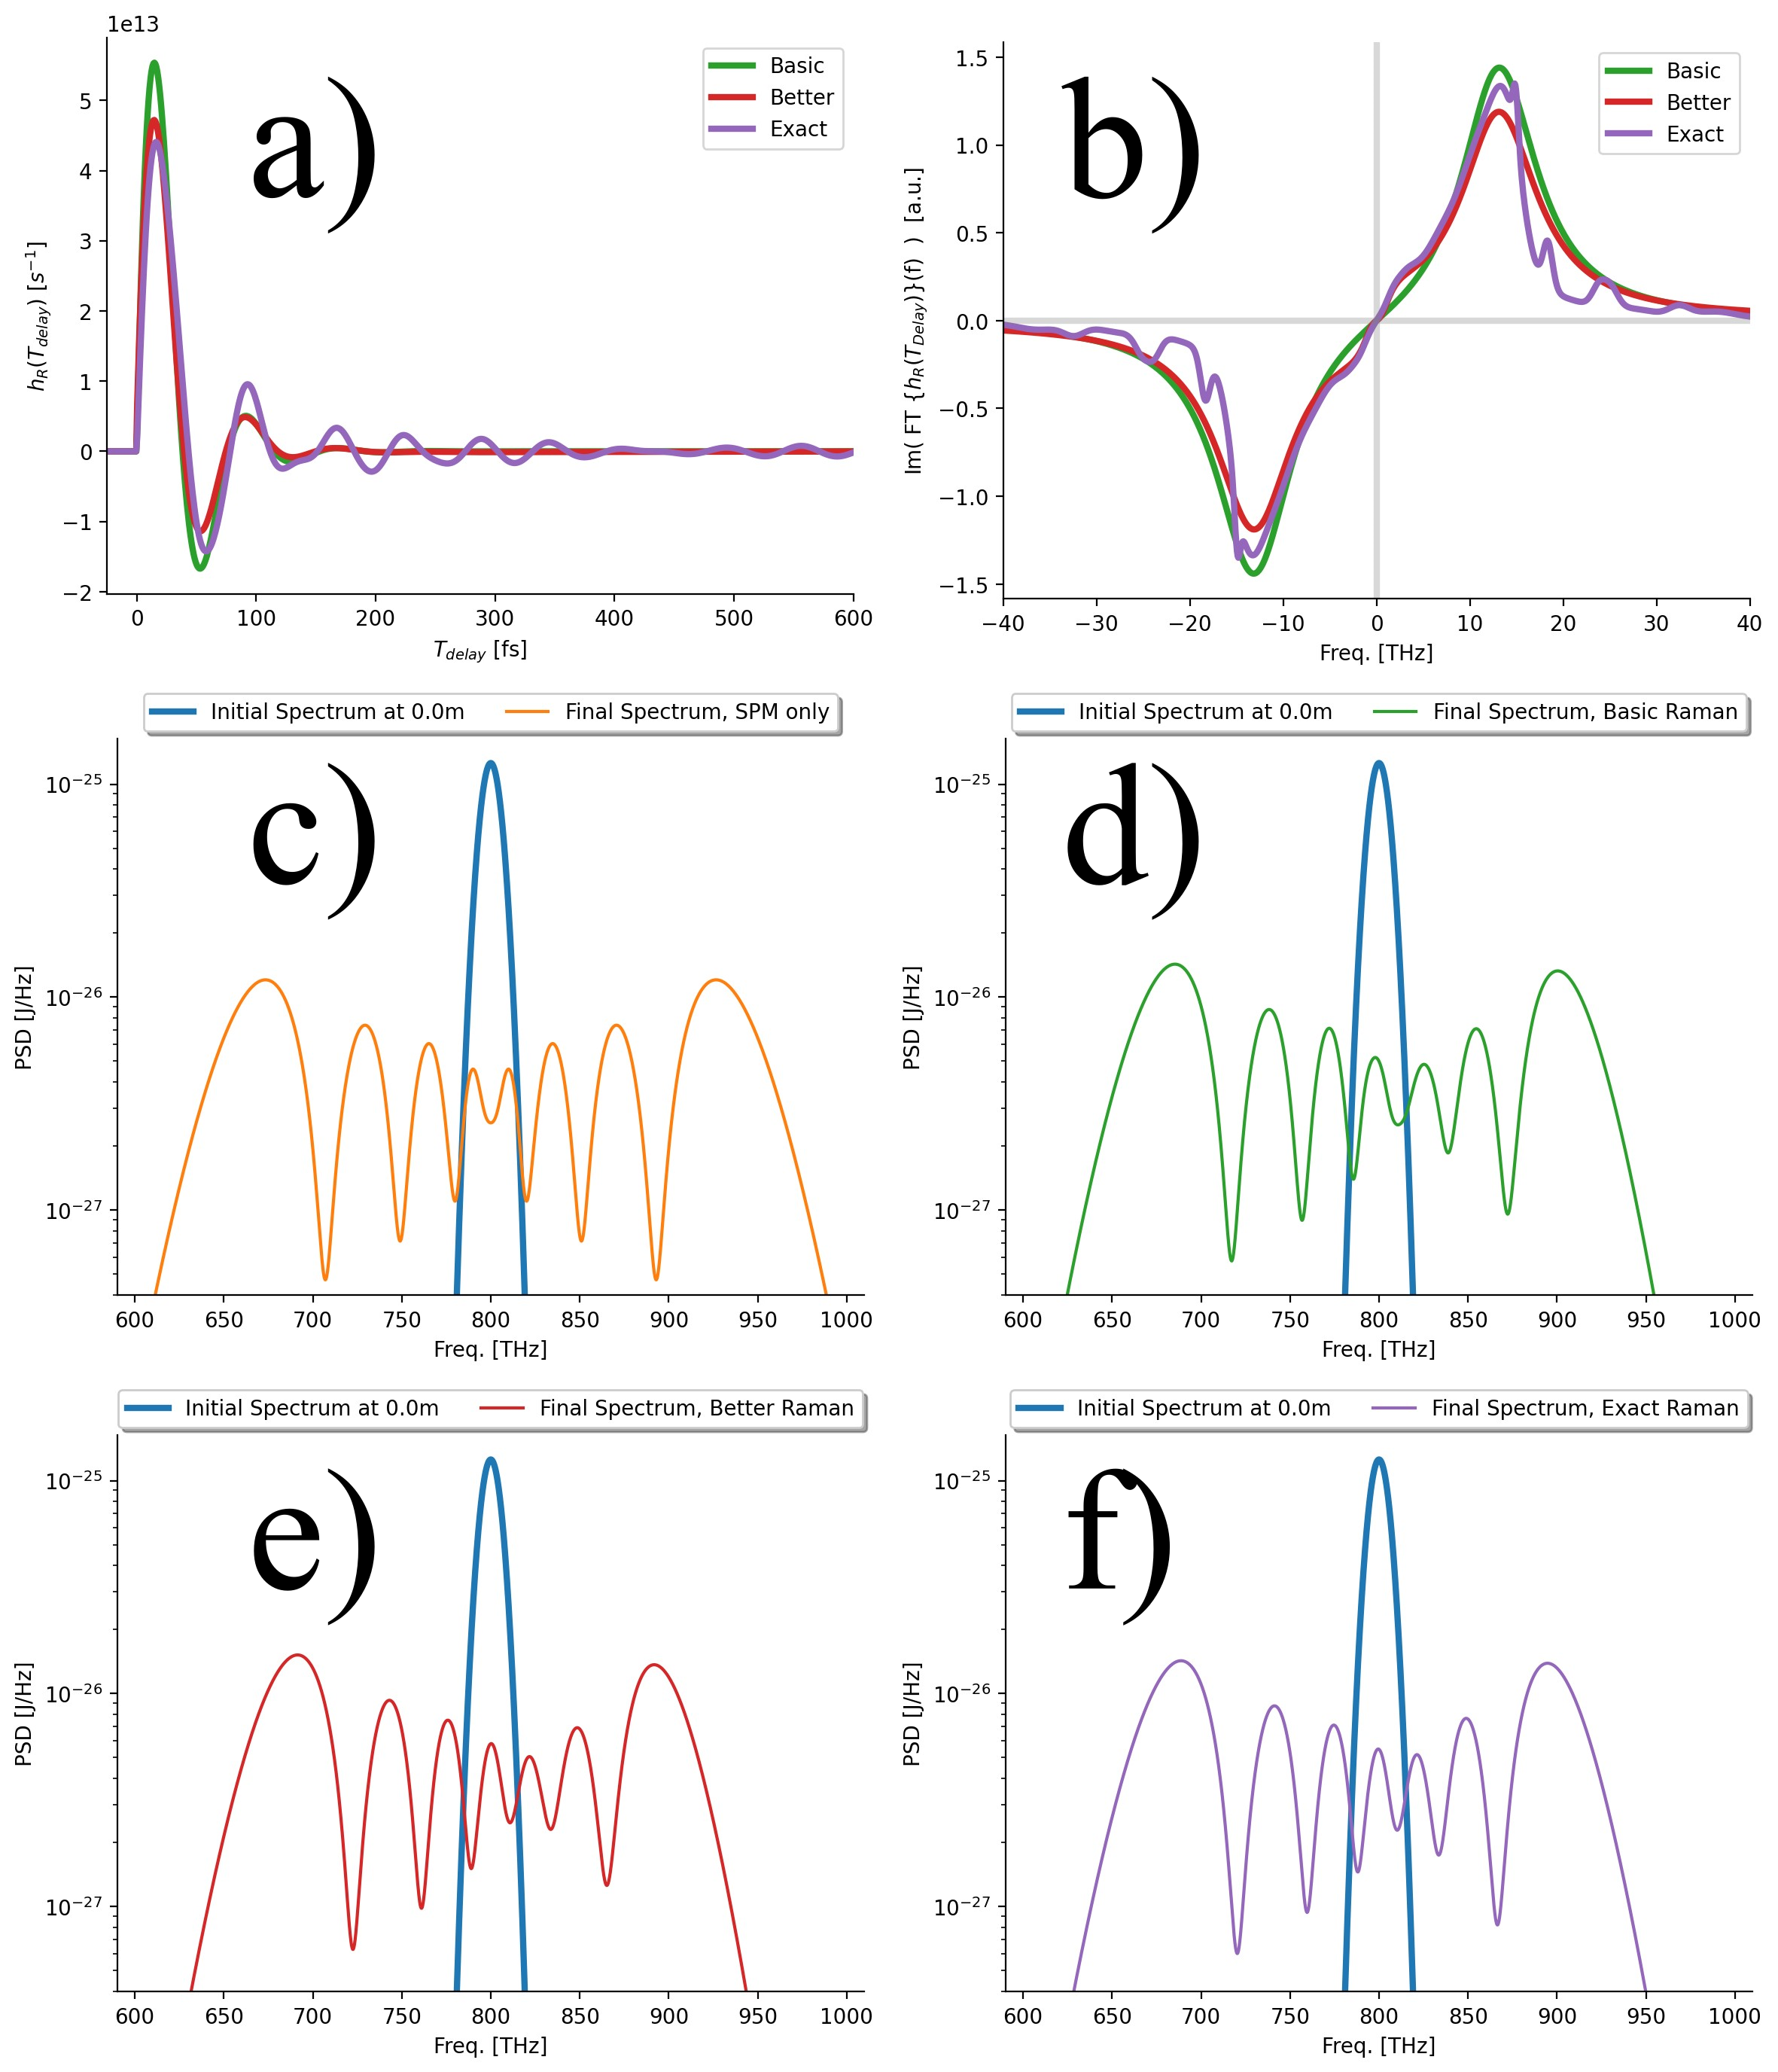
\includegraphics[width=1\linewidth]{figures/Raman_combined.png}
    \caption{a) Eq.~\ref{eq:raman_basic}(绿色)、Eq.~\ref{eq:raman_new}(红色)和 Eq.~\ref{eq:Raman_exact}(紫色)的时域图。) c) 仅受 SPM 影响的脉冲的初始和最终光谱。 d) 受公式 ~\ref{eq:raman_basic} 描述的拉曼效应影响的与 c) 中相同脉冲的初始和最终光谱。e) 与 d) 相同,但 Eq.~\ref{eq:raman_new} f) 与 d) 相同,但 Eq.~\ref{eq:Raman_exact}. 这些图是使用 \href{https://colab.research.google.com/drive/1TqixCGQ51DVwpB3VA6J1XQCpDcf4xwb4?usp=sharing}{这个交互式笔记本}生成的,鼓励读者尝试使用。}
    \label{fig:raman_combined}
\end{figure}






    \chapter{异域脉冲(Exotic pulses)}
\label{ch:Exotic}

对于一根光纤来说,如果$\gamma\neq 0$和$\betag_2\neq 0$,发射到光纤中的脉冲会以多种令人惊讶的方式演变。从本质上讲,非线性会根据脉冲的功率曲线改变脉冲的局部频率,而色散则会导致不同频率相对于载波频率前进或延迟,这反过来又会改变功率曲线。本章将探讨这两种效应在不同的 $\gamma$ 和 $\betag_2$ 值下的相互作用。

\section{基本孤子}
\label{sec:soliton}
考虑一下 $\gamma>0$ 的光纤。如图 ~\ref{fig:chirp_profiles}所示,这将导致脉冲前缘(后缘)产生红(蓝)色偏移。正如在 Sec.~\ref{sec:GVD} 中解释的那样,$\betag_2<0$ 意味着蓝光比红光传播得更快,从而导致脉冲的前缘(后缘)变得更蓝(更红)。如果根据瞬时功率曲线,$\gamma>0$ 会使脉冲的前缘(后缘)更红(蓝),而根据场的二次导数,$\betag_2<0$ 会使脉冲的前缘(后缘)更蓝(红),那么我们自然会问,是否存在一个脉冲包络,在这个脉冲包络中,这两种效应在每个瞬间都完全平衡,因此脉冲的形状在向前传播时不会改变。对于这样的脉冲,场包络应该与距离无关,而相位应该与时间无关,即

\begin{align}
    \A(z,T) &= V(T)e^{i\phi(z)}
\end{align}
解方程 
\begin{align}
\label{eq:NLSE_soliton}
    \partial_z\A &=  -i  \frac{\betag_2}{2}\partial_T^2\A+i\gamma|\A|^2\A.
\end{align}
正如\href{https://github.com/OleKrarup123/NLSE-vector-solver/blob/main/TutorialVideos/Soliton-Video/Fundamental_soliton_derivation.pdf}{此节}推导所解释的那样,可以证明解是
\begin{align}
    \A(z,T) &= \sqrt{\frac{|\betag_2|}{\gamma T_0^2}}\cdot\text{sech}\left(\frac{T}{T_0}\right)\exp\left(i\frac{|\betag_2|}{2T_0^2}z\right),
\end{align}
其中,$T_0$ 是脉冲场下降到其峰值的 64.8\% 时的时间。这种以双曲正割包络为特征的稳定脉冲被称为 “基本孤子”。高斯脉冲与双曲正割脉冲的对比见图 ~\ref{fig:gauss_sech}。请注意,双曲正割脉冲的峰值功率($\A_{max}$)必须选择为正好等于特征振幅($\A_{char}=\sqrt{|\|betag_2|/\gamma T_0^2}$),这样才能实现稳定传播!
\begin{figure}
    \centering
    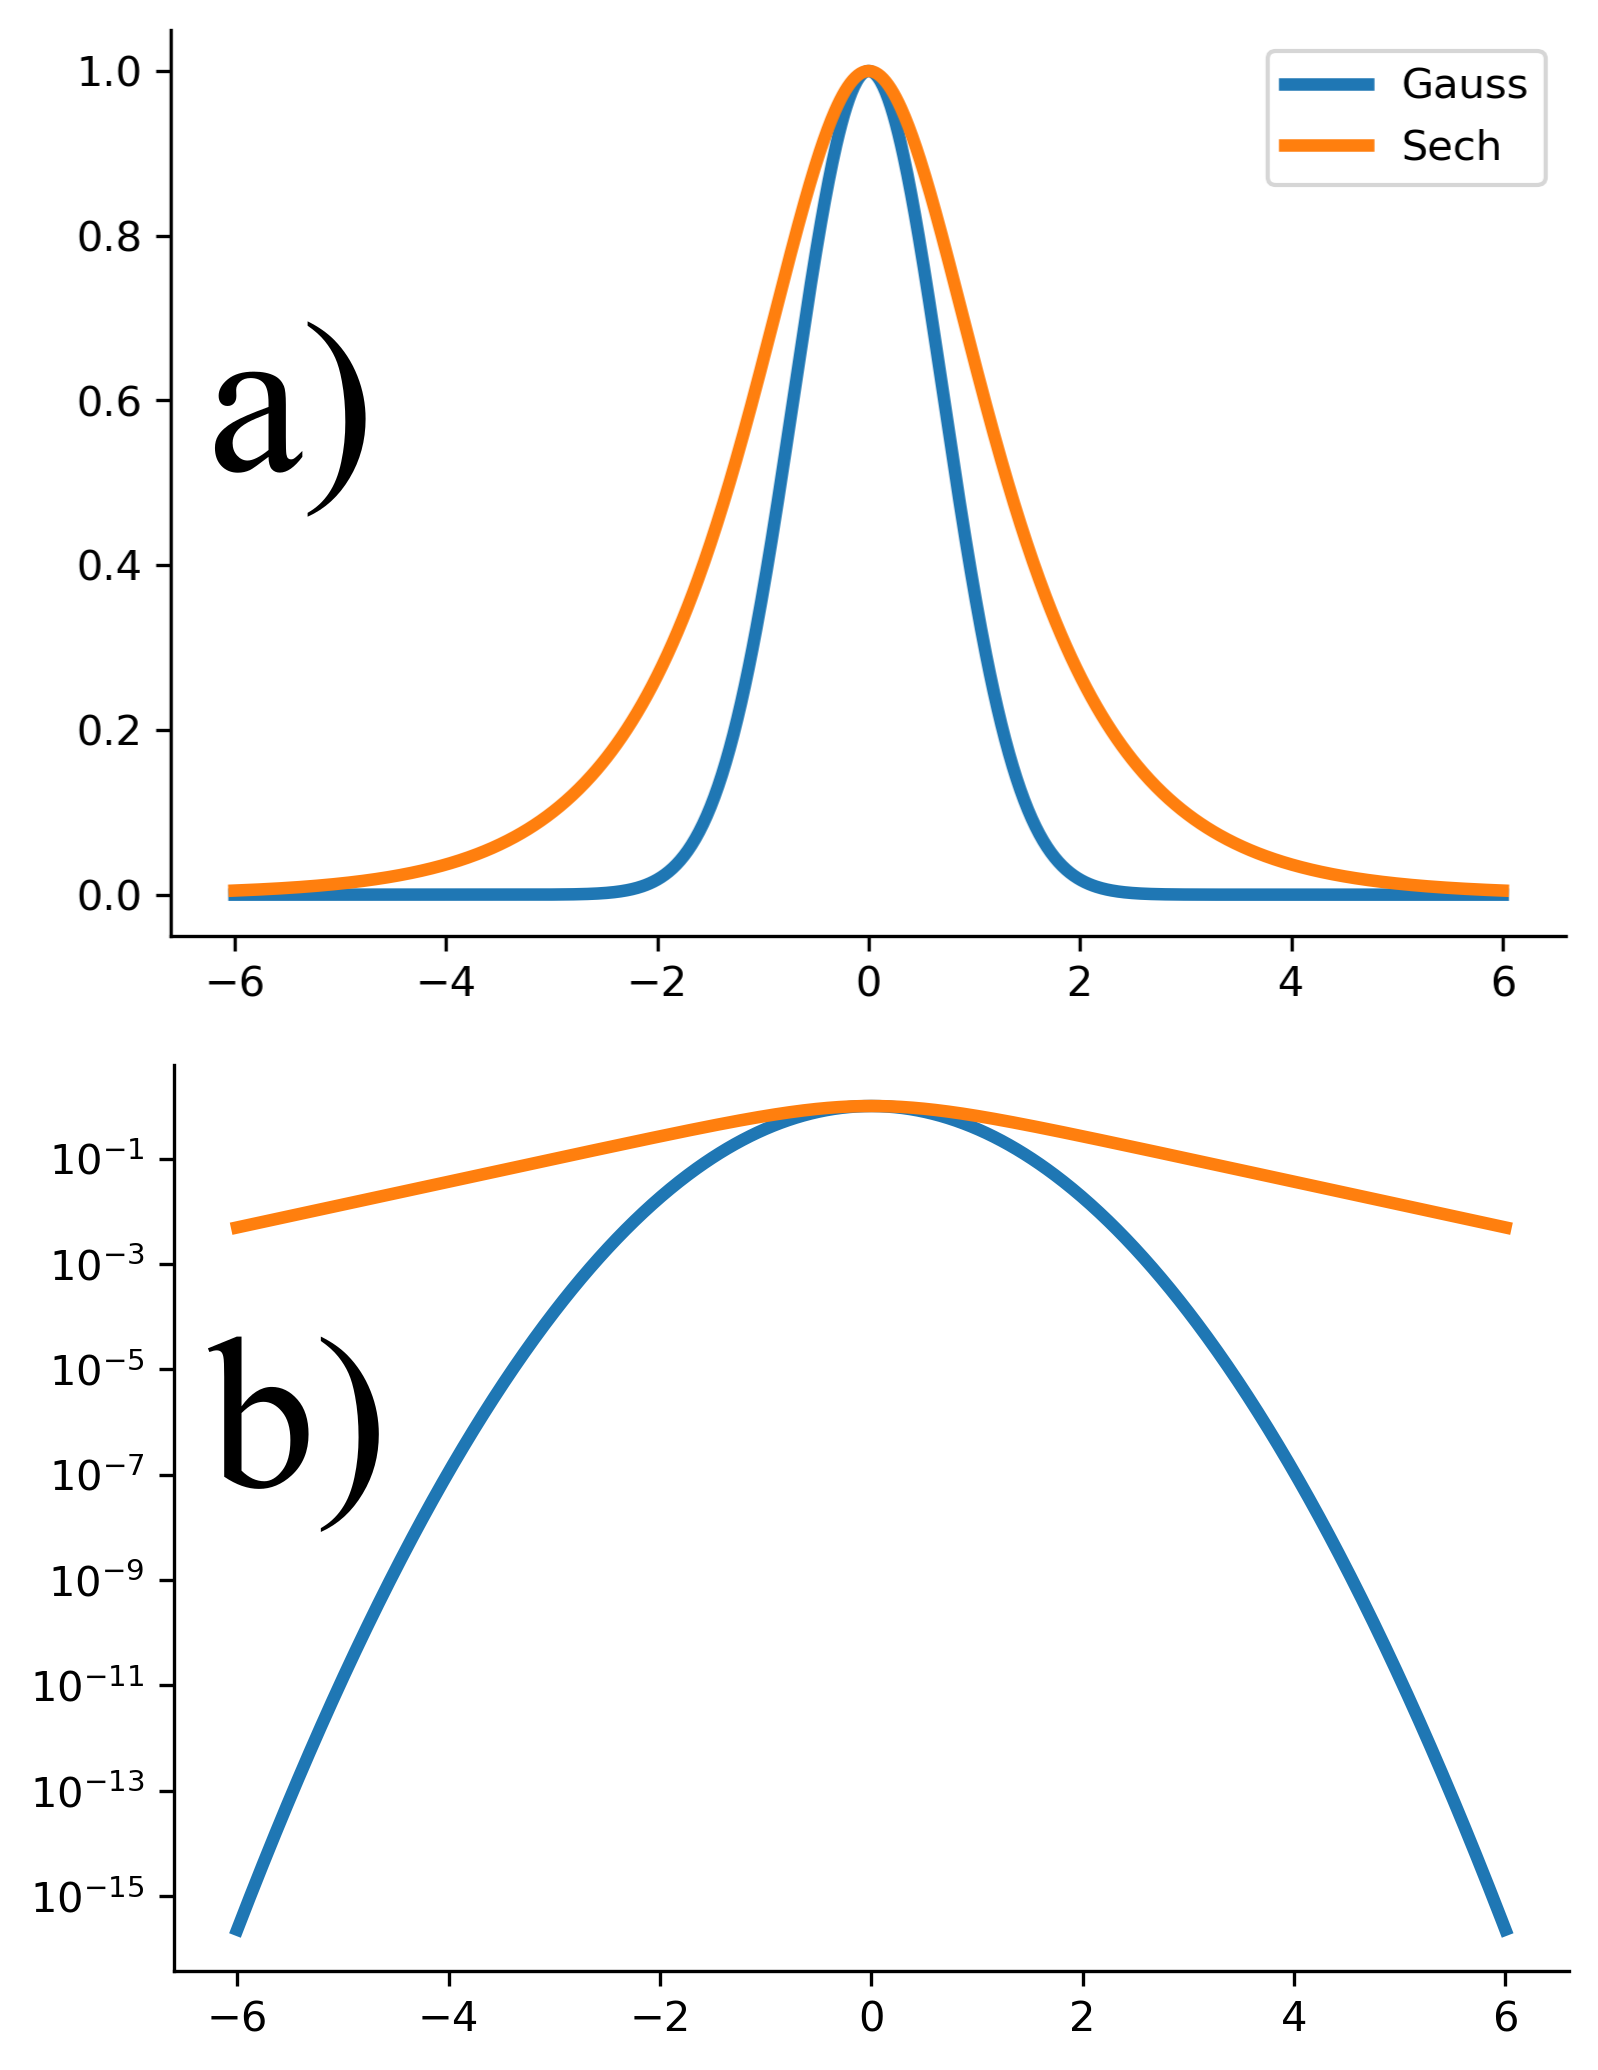
\includegraphics[width=1\linewidth]{figures/gauss_sech_comparison.png}
    \caption{高斯脉冲与双曲正割脉冲的比较,a) 为线性比例,b) 为对数比例。  }
    \label{fig:gauss_sech}
\end{figure}
\subsection{通信中的孤子}
在接近193~THz($\approx$1550~nm)的近红外频率的硅光纤中,由于$\gamma>0$和$\betag_2<0$,基底孤子曾一度在电信领域引起极大兴趣,因为它们的抗色散能力和恒定形状可以减少符号间干扰。然而,在小节{subsec:ZDF}中提到的电子色散补偿方面的改进同样使孤子在光纤通信中的应用过时了。取而代之的是采用所谓“\href{https://www.youtube.com/watch?v=hCk_cg-OfUQ}{root-raised-cosine}”场包络的脉冲。  

\section{Higher order Solitons}
如果双曲正割脉冲的峰值功率小于 $P_{char}=|\A_{char}|^2=|\betag_2|/\gamma T_0^2$,那么与色散相比,非线性效应将过于微弱,无法形成基本孤子。因此,当脉冲向前传播时,它在时域中的范围会扩大。如果峰值功率增大到超过 $P_{char}$,脉冲在演化过程中就会出现 “振荡”。在 $\A_{max}$ 是 $\A_{char}$ 整数倍的特殊情况下,振荡孤子的演化会特别乖巧。关于 $\A_{max}=3\A_{char}$ 的孤子的时间和频谱演化示例,请参见 Fig.~\ref{fig:Soliton_comparison}~a-b)。有关光纤中孤子的更多信息,请参见 \href{https://youtu.be/KAZ7pCQ-x8Y}{本视频教程}。
\subsection{孤子分裂}
\label{subsec:fission}

基阶孤子和高阶孤子可以看作是公式 ~\ref{eq:NLSE_soliton} 的 “固定点(fixed point)”。然而,公式~\ref{eq:NLSE_soliton}本身只是公式~\ref{eq:GNLSE}的近似,而公式~\ref{eq:GNLSE}对影响光脉冲在色散和非线性介质中传播的物理学原理提供了更一般的描述。事实证明,除了 $\gamma>0$ 和 $\betag_2<0$ 之外,其他效应的存在最终会扰乱初始孤子脉冲的演化。在图 ~\ref{fig:Soliton_comparison}~c-d)中,$\betag_3>0$ 的存在会导致一个高阶孤子在传播 0.5 米的距离后,由于 FWM 而 “裂变 ”成两个较弱的新频率孤子。其他效应,如自膨胀效应、拉曼效应,甚至与理想的孤子脉冲一起传播的光噪声所引起的调制不稳定性,也同样会导致孤子裂变。因此,就像一支铅笔在笔尖上保持平衡一样,孤子传播应被视为一种不稳定的平衡。有关孤子裂变的更多详情,请参阅 \href{https://youtu.be/tHpIR2Kuxp0}{本视频教程}。
\begin{figure}
    \centering
    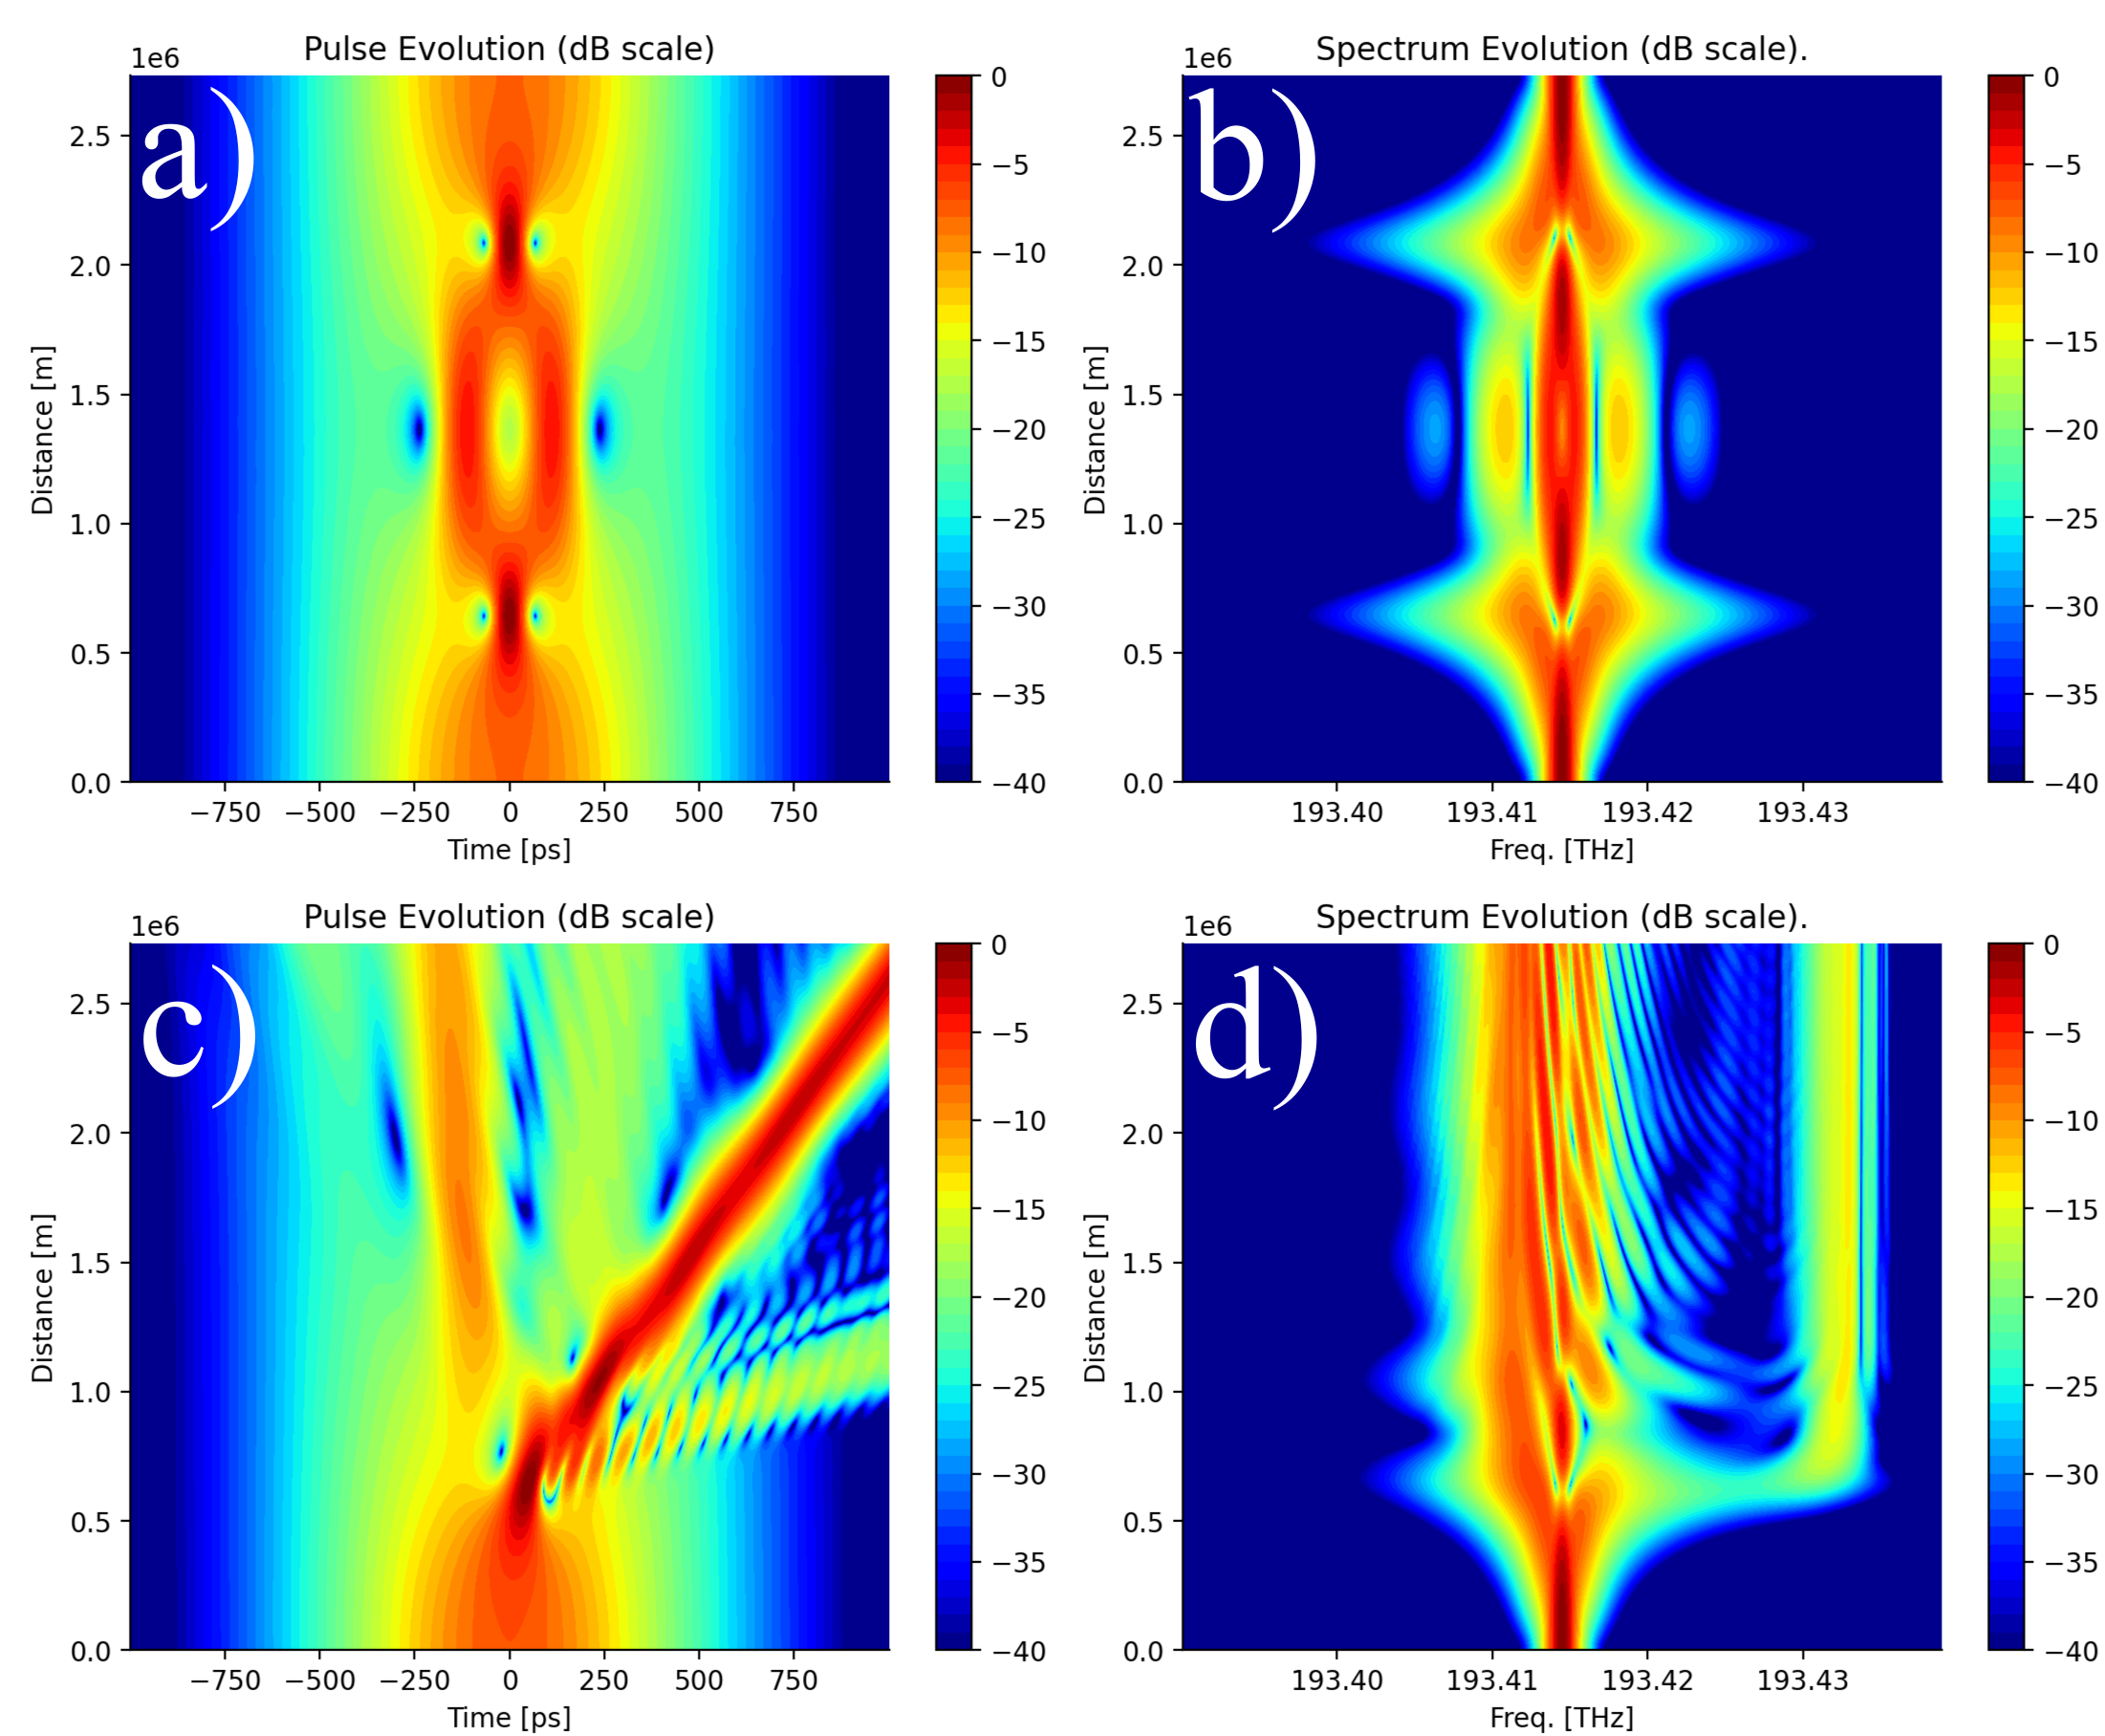
\includegraphics[width=1\linewidth]{figures/Soliton_comparison.png}
    \caption{a) $N=3$ 孤子的时间演变,其中 $\A_{max}=3\A_{char}=3\sqrt{|\betag_2|/\gamma T_0^2}$。b) $N=3$ 孤子的频谱演化。) 与 a-b) 中相同的 $N=3$ 孤子的时间和光谱演变,但光纤的 $\betag_3>0$ 导致脉冲 “裂变”,从而说明了孤子传播的不稳定性。这些图是利用 \href{https://colab.research.google.com/drive/123pT-IsLWIEZY9XW3-1WzkTXfg1IEkkD?usp=sharing}{本互动笔记本}中的数值模拟生成的,我们鼓励读者进行实验。}
    \label{fig:Soliton_comparison}
\end{figure}





\section{光学波破裂(Optical Wave Breaking)}
当海浪接近海滩时,水开始在波浪的前缘“堆积”,最终导致波浪在冲击海岸之前“破裂”。在非线性光纤中,当 $\gamma>0$ 且 $\betag_2>0$ 时,也可以观察到类似的现象。与第~\ref{sec:soliton}节中讨论的当 $\betag_2$ 为负时非线性和色散的平衡不同,现在它们是“协同作用”的。非线性使脉冲的前缘(后缘)变得更红(更蓝),而色散使红色(蓝色)光的传播速度比载波快(慢)。结果是任何脉冲都会在时间域迅速展宽。通常,这种展宽方式会使脉冲的前后功率逐渐“堆积”,从而导致功率斜率变陡,进而生成更大的频率调制(chirp),由于色散的影响,导致脉冲的时间展宽更加快速。当斜率变得足够陡峭时,色散会像水波崩溃一样,将新产生的频率从主脉冲中“推出”。图~\ref{fig:OWB_and_similariton}~a-b)说明了这一现象,称为“光学波破裂”(OWB)。尽管OWB对入射脉冲的变化可能是有害的,但如果想要一个具有陡峭斜率且峰值功率大致恒定的光学脉冲,它也可以是有益的。有关OWB的更多细节,请参阅\href{https://youtu.be/XEx6lOf6f40}{此视频教程}。

\subsection{相似孤子(Similaritons)}
当 $\gamma>0$ 且 $\betag_2>0$ 时,OWB使脉冲在时间域扩展,从而减小其峰值功率。如果进一步假设 $\alpha>0$,意味着脉冲在传播过程中会被放大,那么这种峰值功率的损失会不断被补偿。实际上,在这种情况下,任何输入脉冲(无论其初始形状如何)都会演化为一个具有抛物形功率包络的脉冲,如图~\ref{fig:OWB_and_similariton}~c)所示,并且脉冲的调制将呈现线性变化,从前到后依次变为红色和蓝色~\cite{Similariton_evolution}。这种“相似孤子”的峰值功率和持续时间会随着传播距离的增加而不断增加,具体解释请参见\href{https://youtu.be/ZtWIRaj5VV4}{此视频教程}。相似孤子可以出现在某些光学放大器中,并且由于其线性变化的频率调制,它们是通过诺贝尔奖获得的方法——啁啾脉冲压缩——生成具有极高峰值功率脉冲的理想候选者,详细内容可见\href{https://youtu.be/Eh5CHRWFT-M}{此视频教程}。

\begin{figure}
    \centering
    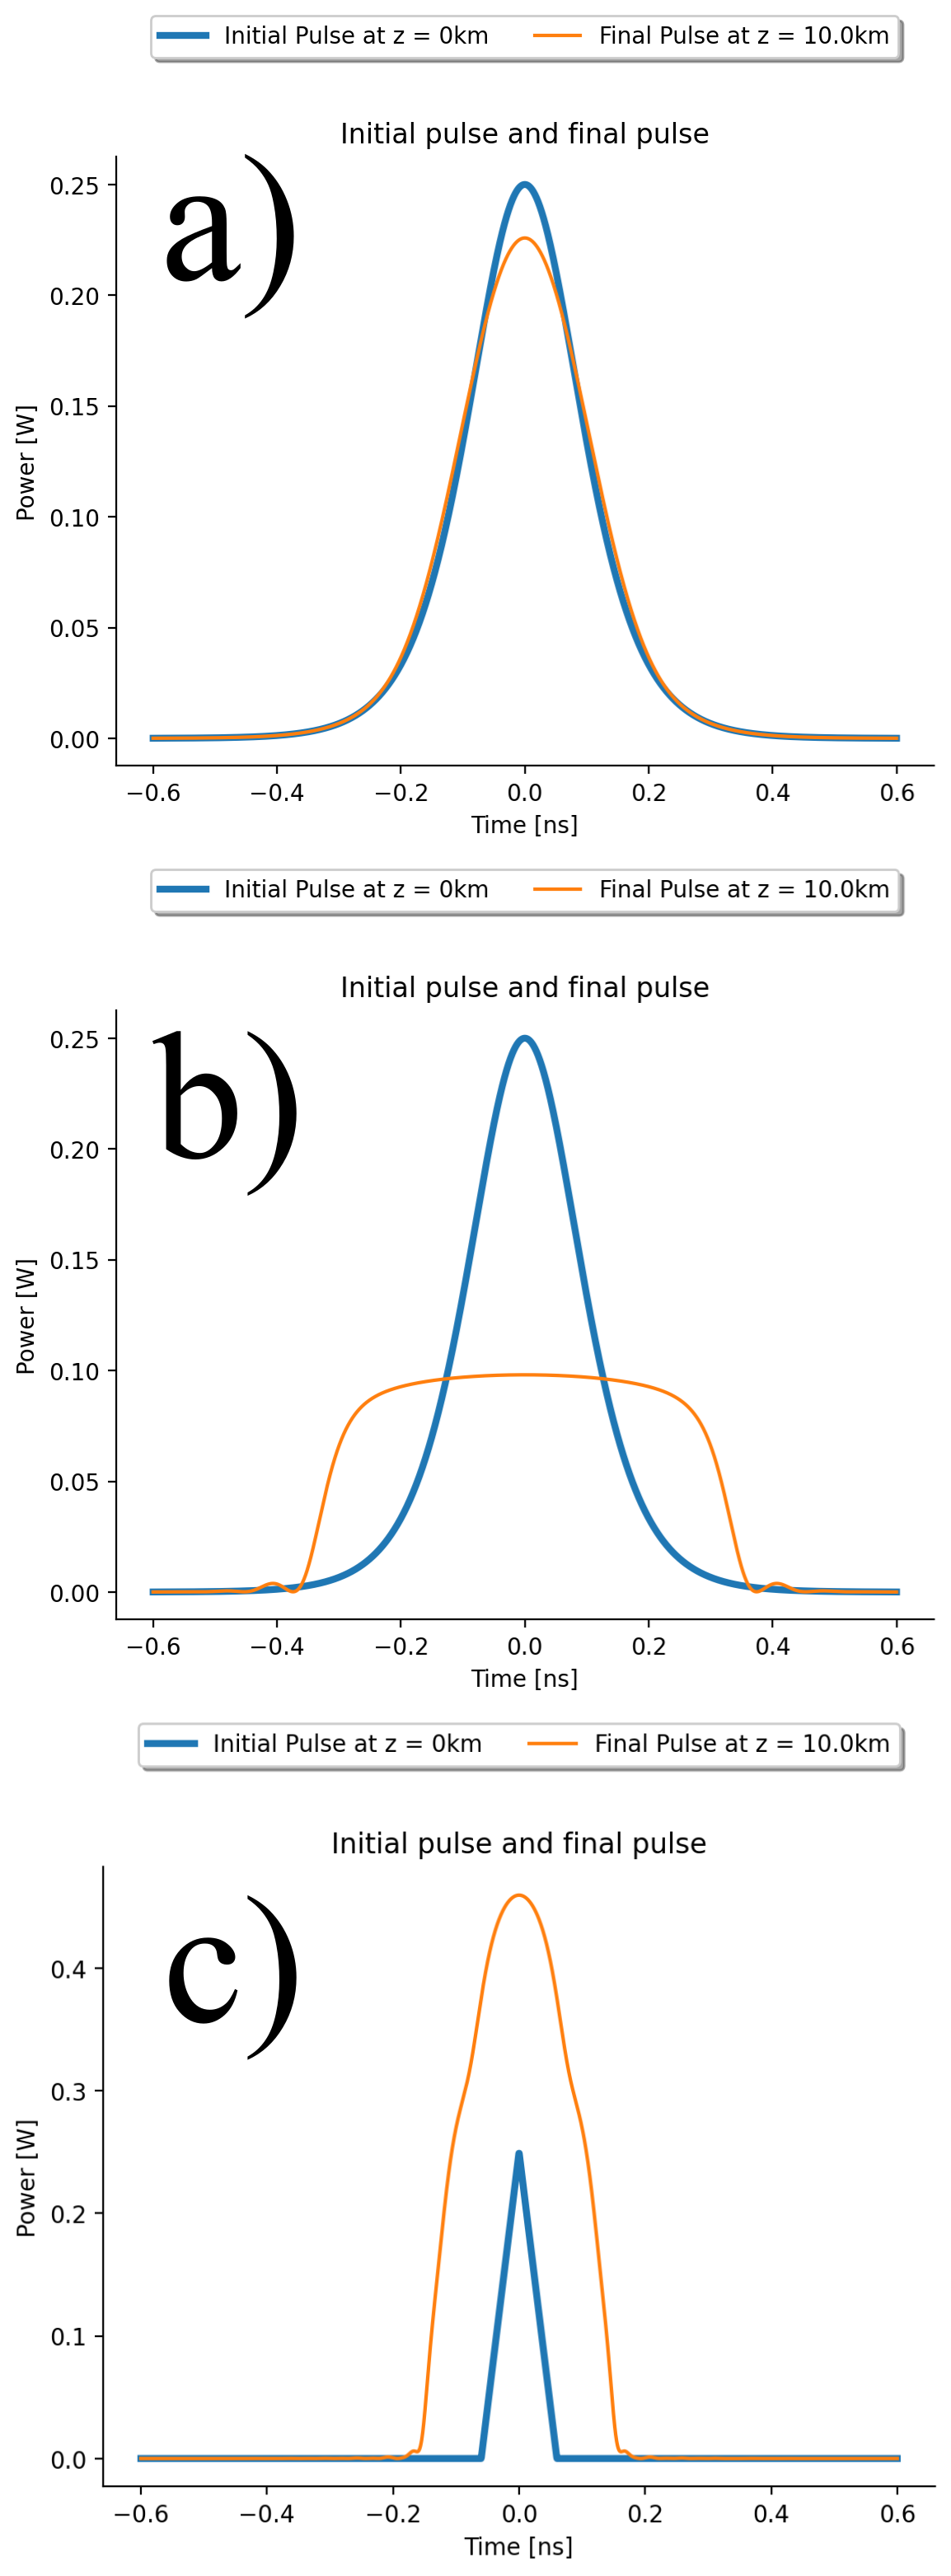
\includegraphics[width=0.5\linewidth]{figures/OWB_and_similariton.png}
    \caption{a)双曲正割脉冲在介质中的演变,其中$\betag_2>0$。b)与a)中相同的脉冲在介质中的演变,其中$\betag_2>0$和$\gamma>0$导致功率在脉冲前后 “堆积”,从而导致OWB。这些图是使用 \href{https://colab.research.google.com/drive/1qtMcXElXn4VBntfCgXIGGkyDfiGicElx?usp=sharing}{本互动笔记本}中的数值模拟生成的,我们鼓励读者进行实验。}
    \label{fig:OWB_and_similariton}
\end{figure}

\section{新型孤子}

\subsection{暗孤子(Dark Solitons)}
通常,光脉冲由突然增加的激光功率组成,前后则是长时间零功率。肉眼看到的脉冲就像是在黑暗的房间里,灯被短暂地打开一样。只要满足第~\ref{sec:soliton}节中描述的条件,这样的脉冲可以稳定地通过非线性介质传播。我们可以考虑在非线性介质中,所谓的“反脉冲”——一个高功率的连续波(CW)信号,经历一个短暂的功率下降,类似于灯短暂熄灭后再被重新点亮。它将由功率下降的前沿和功率上升的后沿组成。如果 $\gamma>0$ 且 $\betag_2>0$,前沿(后沿)会变得更蓝(更红),使得这部分光传播速度变慢(加速)。类似于第~\ref{sec:soliton}节的情况,可以计算出非线性和色散恰好平衡的场包络是一个双曲正切函数,从而形成一个稳定传播的“暗孤子”,其表达式为:

\begin{align}
    \A(z,T) = \A_{char}\tanh\left(\frac{T}{T_0}\right)\exp\left(i\frac{|\betag_2|}{T_0^2}z \right).
\end{align}

有关暗孤子的更多信息,请参见\href{https://youtu.be/MrNfI1_eTZ0}{此视频教程}。

\subsection{拉曼孤子(Raman Solitons)}
如果拉曼效应存在,并且脉冲谱向较低频率移动,那么在 $\betag_2<0$ 的非线性介质中可以形成一个“拉曼孤子”。这个孤子保持其包络的形状,但会经历一个恒定的红移,并由于 $\betag_2<0$ 使得红光比蓝光传播得更慢,进而产生越来越大的时间延迟,如图~\ref{fig:dark_and_raman}c-d)所示。拉曼孤子通常出现在脉冲的孤子裂变之后,这些脉冲的持续时间通常在几十飞秒的量级。有关拉曼孤子的解释,请参见\href{https://www.youtube.com/watch?v=K33YUfegL1w}{此视频教程}。

\begin{figure}
    \centering
    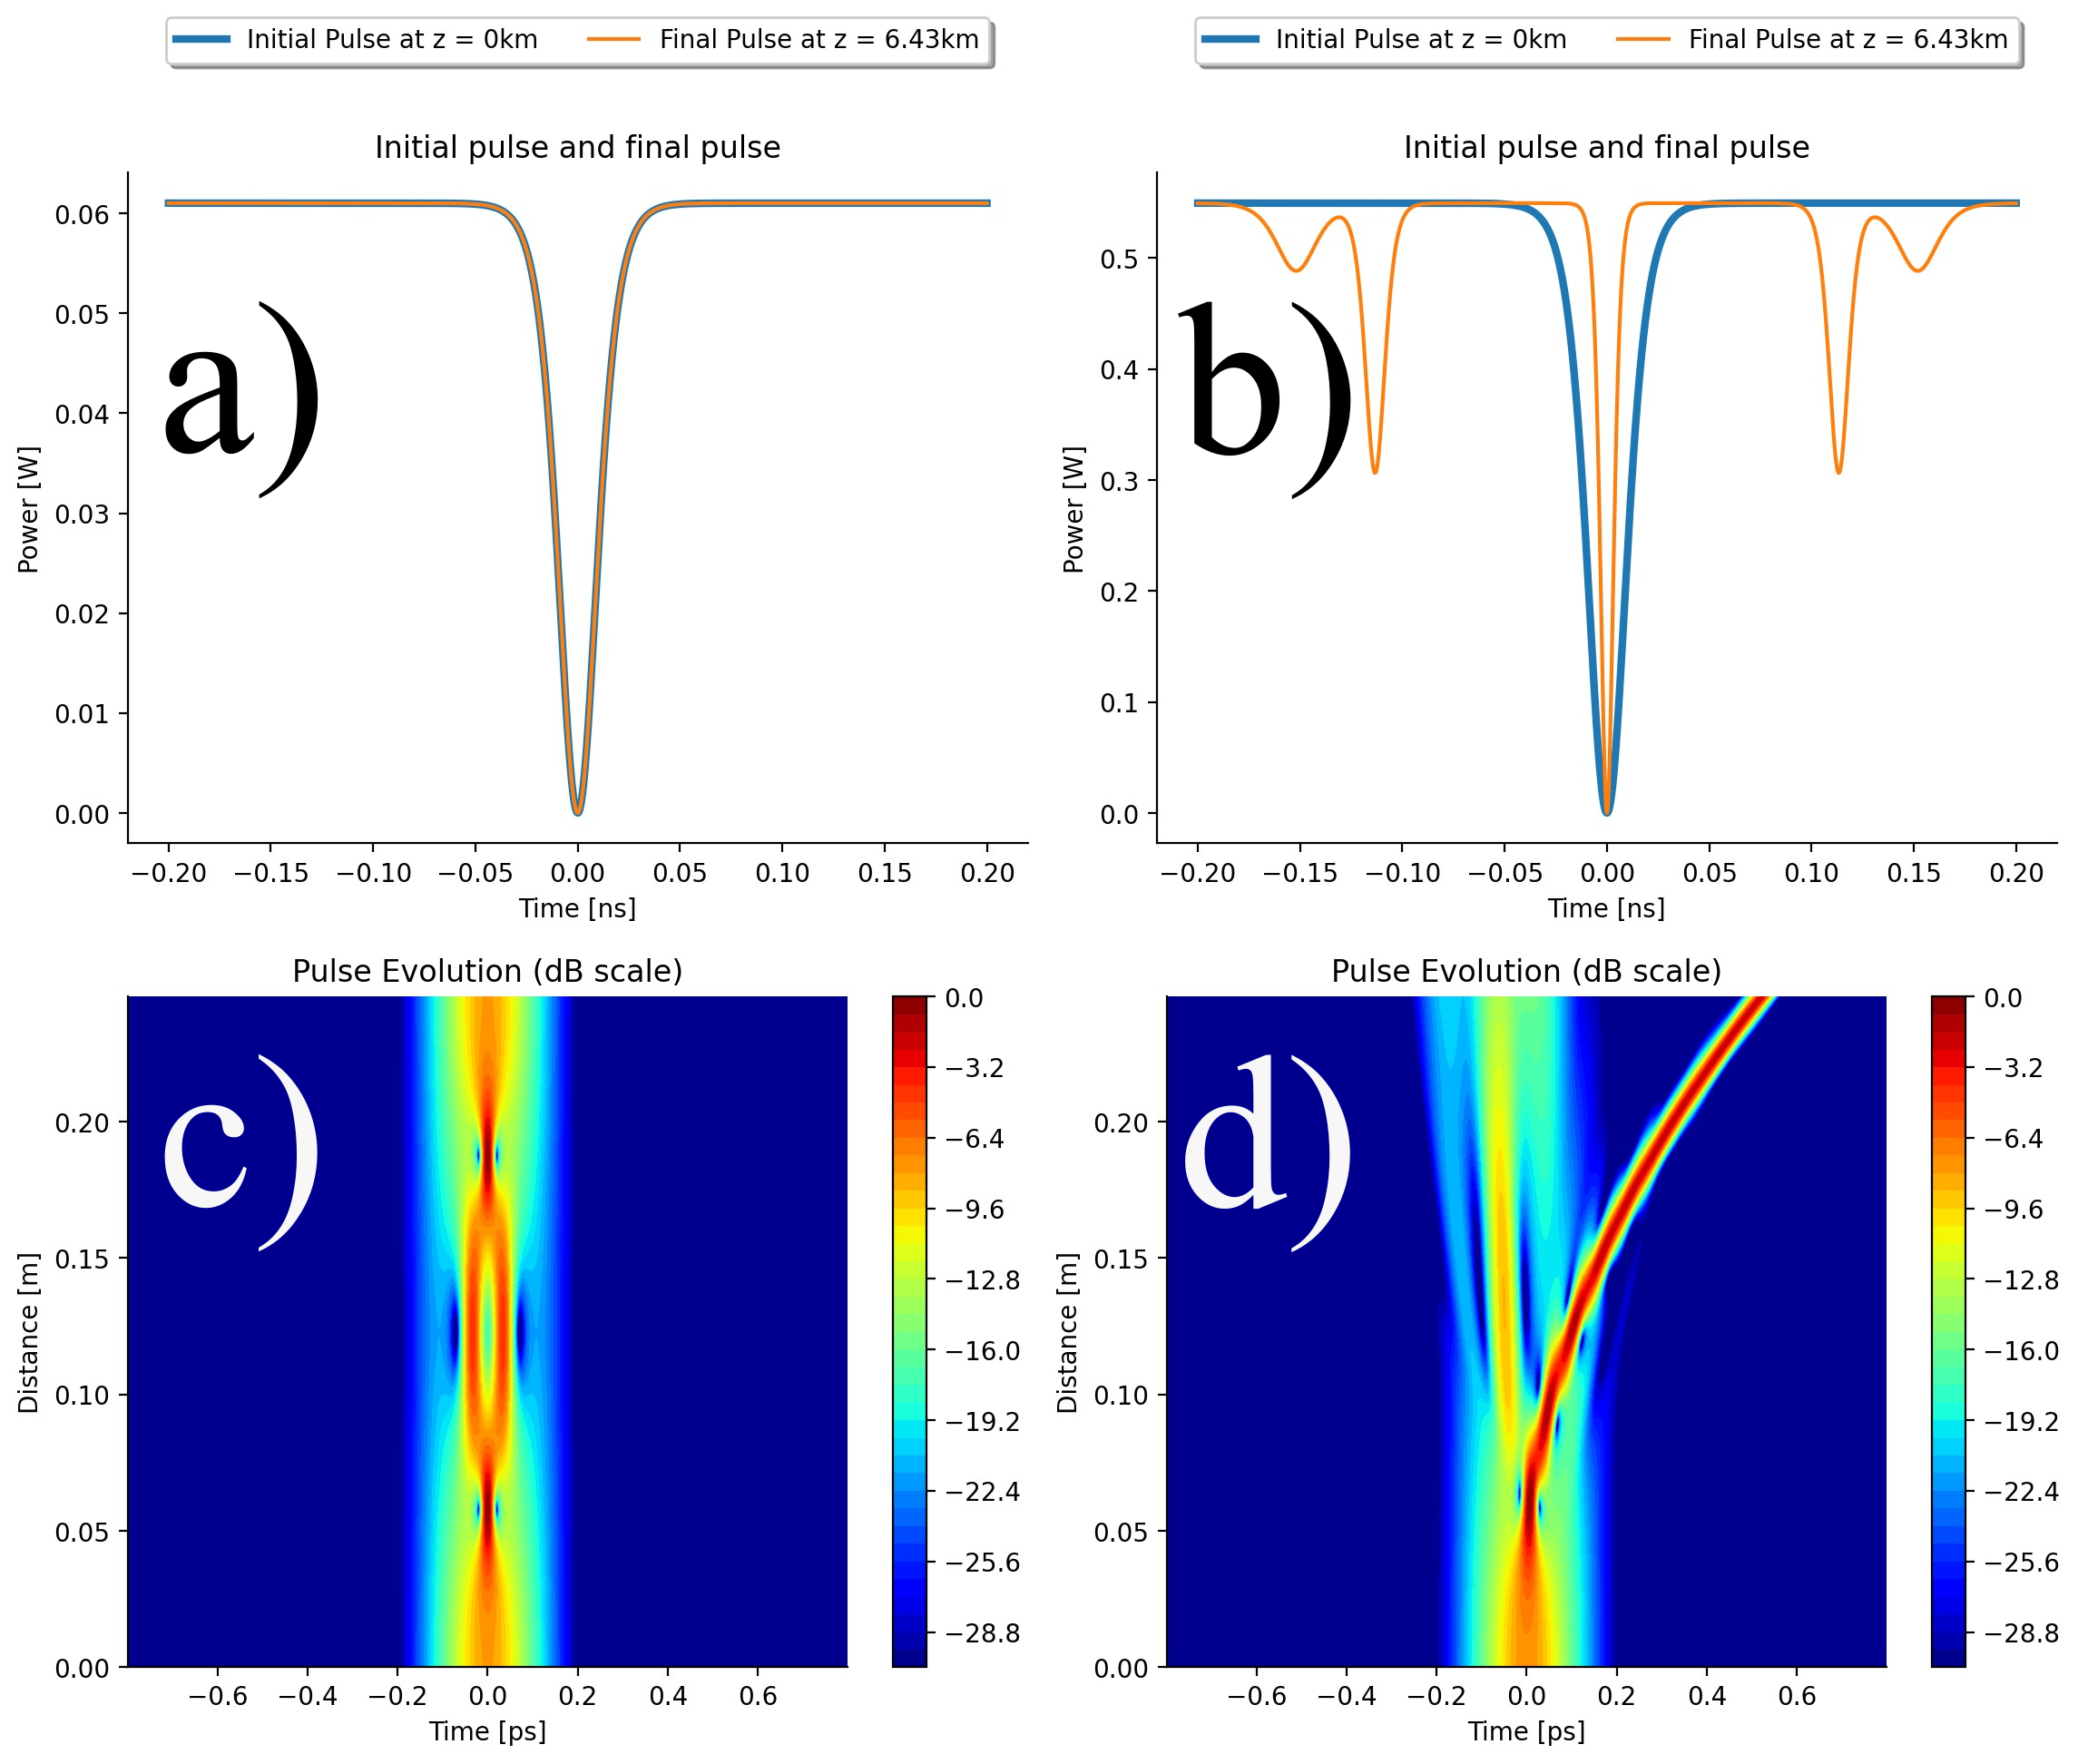
\includegraphics[width=1\linewidth]{figures/dark_and_raman_soliton_combined.png}
    \caption{a) 基本暗孤子在介质中稳定传播,其中 $\betag_2>0$ 和 $\gamma>0$. b) 一个 N=3 的暗孤子在介质中传播,与 a 中相同。c) 一个 N=3 的孤子在$\betag_2<0$和$\gamma>0$的介质中传播。 d) 与 c) 中相同的脉冲在相同的介质中传播,除了公式 ~\ref{eq:raman_basic} 所描述的拉曼效应被考虑在内,导致孤子裂变并产生一个自漂移拉曼孤子。这些图是使用 \href{https://colab.research.google.com/drive/1qtMcXElXn4VBntfCgXIGGkyDfiGicElx?usp=sharing}{这个互动笔记本}生成的,我们鼓励读者进行实验。}
    \label{fig:dark_and_raman}
\end{figure}

\subsection{矢量孤子(Vector Solitons)}
在第~\ref{Sec:XPM}节中,已经展示了不同频率的光可以通过非线性效应相互影响相位。同样,在非线性介质中,两种不同的光偏振也可以相互影响相位。通过使用方程~\ref{eq:GNLSE} 的矢量版本,其中 $\gamma>0$,$\betag_2<0$,且介质中光沿 x 和 y 轴的折射率不同,可以得到所谓的“矢量孤子”的解析表达式。对于这些情况,孤子的特殊情况是圆偏振光和偏振方向为 $45^{o}$ 的线性偏振光~\cite{AGRAWAL_CH6_POL}。







    \chapter{超连续谱生成}
\label{ch:supercontinuum}

前面的章节解释了单个线性和非线性效应及其相互作用,并总结了它们的影响,如表~\ref{tab:NL_summary}所示。对于具有载频使得$\betag_2\lesssim 0$且$\gamma>0$的高功率脉冲,以及持续时间低于约100~fs的情况,这些效应可能同时存在。在这种情况下,脉冲的演化可能非常复杂,并将其谱宽度扩展到其初始带宽的十到二十倍~\cite{supercontinuum_original_paper}。本章通过一个超连续谱生成的例子,阐述了如何通过之前讨论的效应理解这一过程。

\begin{table}[]
\begin{adjustwidth}{-2cm}{}
\begin{tabular}{ccccc}
\hline
\textbf{效应}       & \textbf{时域表现}                                                                                      & \textbf{光谱表现}                                                                                           & \textbf{对以下情况显著}                                                                           & \textbf{相关性}                                                                                                       \\ \hline
$\alpha>0$            & 增加功率.                                                                                           & 增加功率.                                                                                             & 放大器                                                                                         & \begin{tabular}[c]{@{}c@{}}非线性效应高度\\ 依赖于功率.\end{tabular}                                            \\ \hline
$\beta_2<0$           & \begin{tabular}[c]{@{}c@{}}脉冲前端(蓝)和后端(红)\\ 各自展宽.\end{tabular}            & \begin{tabular}[c]{@{}c@{}}光谱相位\\ 随与载频的\\ 距离变化.\end{tabular} & \begin{tabular}[c]{@{}c@{}}短的NIR脉冲\\ 在二氧化硅中.\end{tabular}                             & \begin{tabular}[c]{@{}c@{}}非线性效应在\\ $\beta_2+\gamma P\approx 0$时显著.\end{tabular}                      \\ \hline
$\beta_3$             & \begin{tabular}[c]{@{}c@{}}根据符号推迟或提前\\ 非载频成分.\end{tabular}    & \begin{tabular}[c]{@{}c@{}}光谱相位与\\ 载频的\\ 距离三次方变化.\end{tabular}        & \begin{tabular}[c]{@{}c@{}}载频接近\\ 零色散频率(ZDF).\end{tabular}                            & \begin{tabular}[c]{@{}c@{}}不同频率在时域中\\ 重叠导致FWM.\\ 孤子分裂.\end{tabular} \\ \hline
自相位调制(SPM) & \begin{tabular}[c]{@{}c@{}}脉冲前缘(红)和后缘(蓝)\\ 各自偏移.\end{tabular}                     & \begin{tabular}[c]{@{}c@{}}对称\\ 展宽.\end{tabular}                                            & 高功率脉冲                                                                                  & \begin{tabular}[c]{@{}c@{}}最基本的非线性效应. \\ 首先“启动”随着\\ 功率增大.\end{tabular}            \\ \hline
自陡化       & \begin{tabular}[c]{@{}c@{}}脉冲峰值延迟\\ 到后期时间,\\ 导致陡峭的后坡.\end{tabular} & \begin{tabular}[c]{@{}c@{}}偏向高频的\\ 展宽.\end{tabular}                 & \begin{tabular}[c]{@{}c@{}}短时脉冲与载频\\ 比较.\end{tabular} & \begin{tabular}[c]{@{}c@{}}SPM的细微修正。\\ 孤子分裂.\end{tabular}                            \\ \hline
拉曼效应     & 脉冲峰值红移。                                                                                  & \begin{tabular}[c]{@{}c@{}}偏向低频的\\ 展宽.\end{tabular}                  & \begin{tabular}[c]{@{}c@{}}极短脉冲在\\ 10-100fs量级.\end{tabular}     & \begin{tabular}[c]{@{}c@{}}拉曼红移效应\\ 可以超过SPM\\ 展宽.  \\ 孤子分裂.\end{tabular}            \\ \hline
\end{tabular}
\caption{不同线性和非线性效应的影响总结。}
\label{tab:NL_summary}
\end{adjustwidth}
\end{table}

\section{案例研究}
为了模拟超连续谱的生成,使用了表~\ref{tab:SC_params}中的参数。生成的超连续谱如图~\ref{fig:SC_combined}所示。图~\ref{fig:SC_combined} c)中的光谱表明,脉冲在前1~m的传播过程中经历了SPM效应,而图~\ref{fig:SC_combined} b)表明,孤子分裂发生在随后的区域。高功率脉冲具有比初始脉冲小得多的持续时间,它沿着抛物线向后延伸,形成一个拉曼孤子,并不断发生红移。线性"走离"的低功率光可能是由FWM生成的,这一过程发生在分裂的孤子与初始脉冲残余部分重叠时。有关此超连续谱的详细分析,请参阅\href{https://youtu.be/-GDsMDpC3oA}{此视频教程}。

\begin{table}[]
\centering
\begin{tabular}{cc}
\textbf{参数}                      & \textbf{数值}                                  \\ \hline
时间点数                           & $2^{14}$                                          \\ 
时间分辨率 {[}fs{]}                & 1.8                                             \\ \hline
脉冲类型                              & Sech                                            \\ 
持续时间 {[}fs{]}                       & 166.79                                          \\ 
峰值功率 {[}W{]}                      & 50                                              \\ 
载频 {[}THz{]}                 & 282.823 (=1060~nm)                         \\ \hline
$\alpha$ {[}dB/km{]}                    & 0                                               \\ 
$\betag_2$ {[}s\textasciicircum{}2/m{]} & -3.051721e-27                                   \\ 
$\betag_3$ {[}s\textasciicircum{}3/m{]} & 7.29029e-41                                     \\ 
$\betag_4$ {[}s\textasciicircum{}4/m{]} & -1.08817e-55                                    \\ 
$\betag_5$ {[}s\textasciicircum{}5/m{]} & 2.8941e-70                                      \\ 
$\betag_6$ {[}s\textasciicircum{}6/m{]} & 4.8348e-89                                      \\ 
$\betag_7$ {[}s\textasciicircum{}7/m{]} & -1.1464e-113                                    \\ 
$\betag_8$ {[}s\textasciicircum{}8/m{]} & 1.8802e-128                                     \\ 
$\betag_9$ {[}s\textasciicircum{}9/m{]} & -1.5054e-143                                    \\ 
$\gamma$ {[}1/W/m{]}                    & 0.09                                            \\ 
自陡化                         & 开启                                              \\ 
拉曼模型                             & 方程~\ref{eq:raman_basic}
\end{tabular}
\caption{用于生成超连续谱的模拟参数,取自~\cite{supercontinuum_paper}}
\label{tab:SC_params}
\end{table}

\begin{figure}
    \centering
    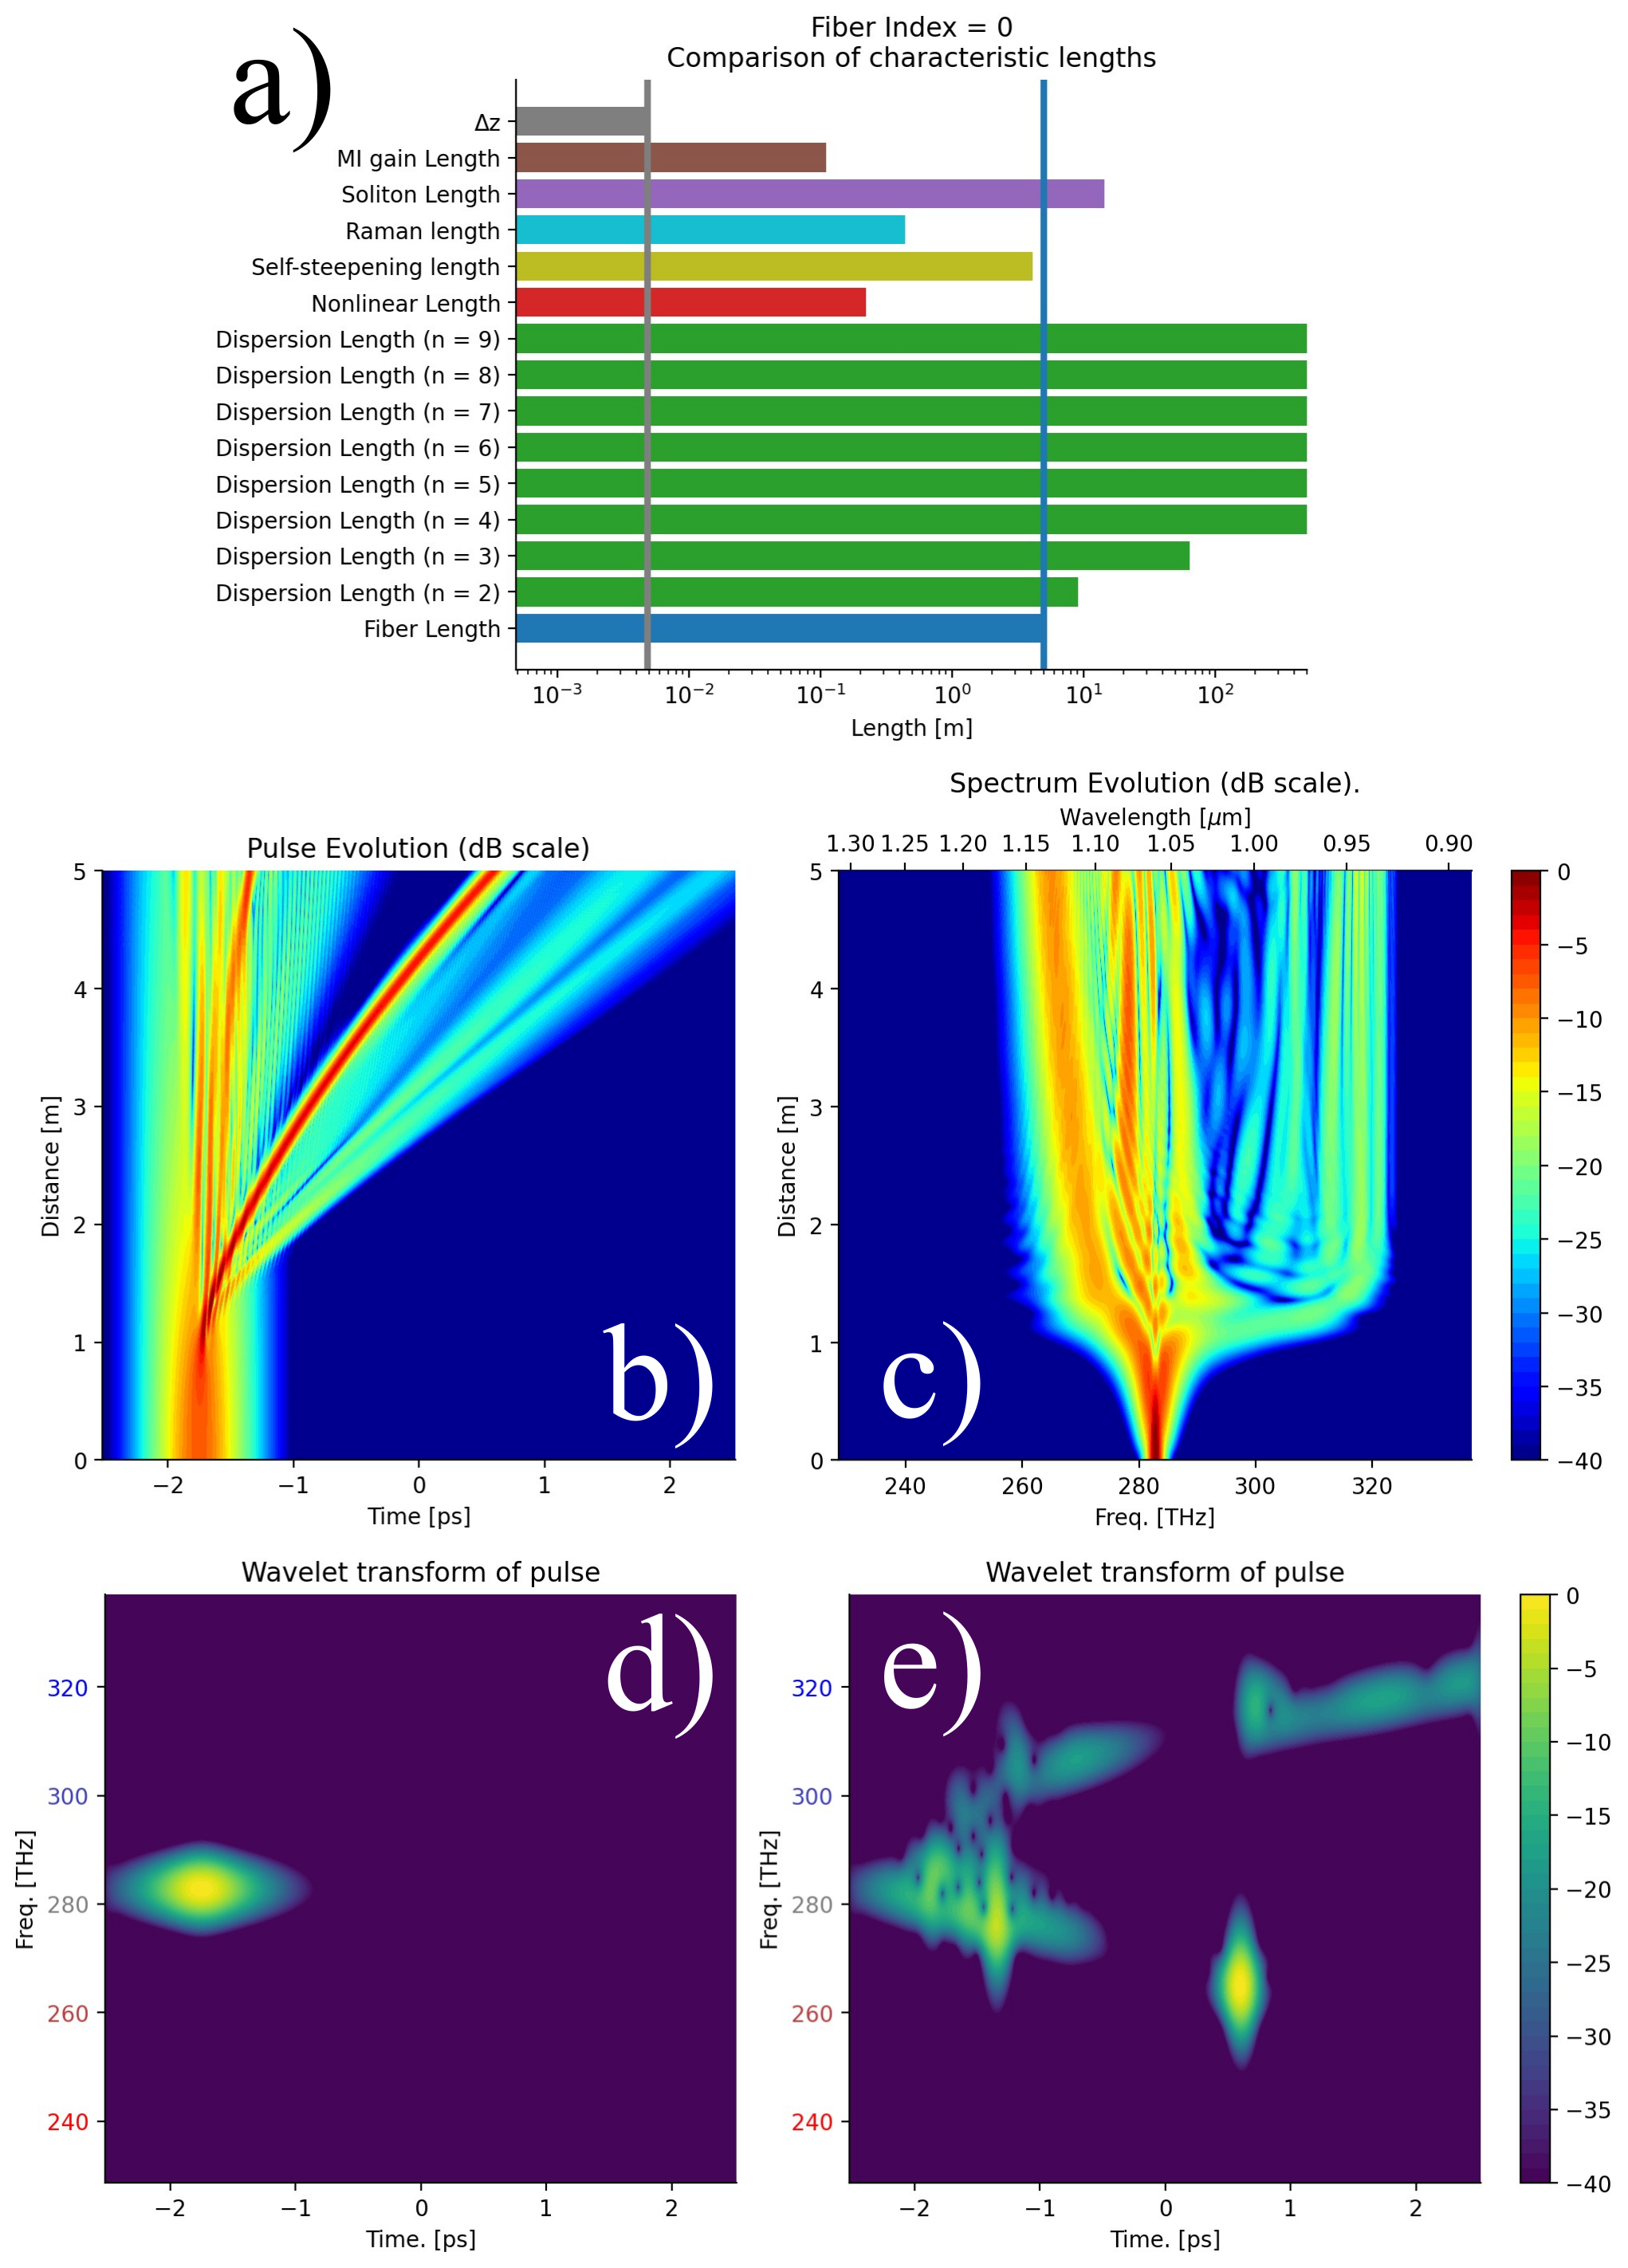
\includegraphics[width=0.9\linewidth]{figures/SC_combined.png}
    \caption{a) 使用表~\ref{tab:SC_params}中列出的参数比较特征长度。具有短特征长度的效应将首先变得显著。b) 脉冲的时间演化,显示在约1~m的距离处发生孤子分裂,之后是FWM并生成拉曼孤子,逐渐向后延伸。c) 脉冲的光谱演化。d) 初始时刻$z=0$的光谱图。e) $z=5$~m时的光谱图。}
    \label{fig:SC_combined}
\end{figure}

\section{你的实验}
为了进一步探索图~\ref{fig:SC_combined}中模拟的超连续谱特性,请打开生成该图的\href{https://colab.research.google.com/drive/1HvA8F8yzEq-9fahuI4z2KhT-YhdRAXgt?usp=sharing}{Colab笔记本},并进行以下实验,解释脉冲及其光谱演化的不同。每次实验前,请写下你对模拟结果的预期,以便与实际结果进行对比。请注意,在每次实验前“重置”参数到默认值:

\begin{enumerate}
\item \textbf{无非线性效应}。当前模拟使用了$\gamma>0$。将其改为$\gamma=0$。结果是否表明非线性效应对脉冲的时间演化有重要影响?

\item \textbf{无自相位调制效应}。当前模拟考虑了自相位调制的影响。关闭此效应后,观察其对结果的影响。

\item \textbf{负$\alpha$值}。当前模拟中使用$\alpha=0$。将其改为$\alpha=-1$~dB/m。观察该修改对结果的影响。

\item \textbf{正的$\betag_2$值}。当前模拟中使用$\betag_2<0$。将$\betag_2$的符号改为正值。

\item \textbf{仅$\betag_2<0$}。当前模拟中使用了$\betag_n\neq 0$($n>2$)。将$\betag_n = 0$($n>2$),运行模拟并解释脉冲及其光谱演化的变化。

\item \textbf{负$\betag_3$值}。当前模拟中使用$\betag_3>0$。将$\betag_3$改为正值。注意:为了确保正确绘制时间演化图,可能需要将时间偏移从-1.75~ps改为+1.75~ps。你能解释为什么当$\betag_3<0$时不会出现拉曼孤子吗?提示:使用公式~\ref{eq:ZDF}计算零色散频率并考虑符号变化对其的影响。

\item \textbf{修改拉曼模型}。当前模拟使用了方程~\ref{eq:raman_basic}来建模拉曼效应。根据笔记本中的提示,使用方程~\ref{eq:raman_new}、方程~\ref{eq:Raman_exact}或$f_R=0$来修改模型。
\end{enumerate}

    \chapter{推荐资料}
\label{ch:material}
以下是关于光学、电子学和通信领域的有用且易获取的资源列表。

\section{光学}

\subsection*{光子学要素}
这本由伊豆香敬教授编写的教科书,介绍了实际光学器件背后的理论,涵盖了广泛的话题。特别推荐其对掺铒光纤放大器(EDFA)增益和噪声特性的讨论,EDFA是现代光学和电信中不可或缺的工具。

\subsection*{现代光学讲座,帕尔塔·罗伊·乔杜里教授}
这系列\href{https://www.youtube.com/watch?v=2WiMeh1Dxl8&list=PLbRMhDVUMngePMuAGeAUeGVuZffTFY-5i}{60个免费视频讲座}涵盖了麦克斯韦方程、偏振和双折射等基础内容,还包括波导和电光调制器等器件的更高级主题。强烈推荐,因其结构良好且数学推导严谨,涵盖了所有描述的主题。

\subsection*{非线性光学讲座,萨穆德拉·罗伊教授}
这系列\href{https://www.youtube.com/watch?v=EiIDScj124Q&list=PLbRMhDVUMngfBwyonVP8VIsabtnsV3GVv}{60个免费视频讲座}首先讲解了线性光学中的基本概念,然后从麦克斯韦方程出发,详细推导了二阶和三阶非线性效应。讲解了二次谐波生成(SHG)、差频生成(DFG)、光学参量振荡器(OPO)以及一些超出本教材范畴的现象。特别推荐其对$\chi^{(2)}$和$\chi^{(3)}$非线性对称性和张量性质的解释。

\subsection*{非线性光纤光学}
这本由戈温德·P·阿格拉瓦尔编写的教科书详细解释了方程~\ref{eq:GNLSE}背后的数学原理,并且频繁参考实验结果。强烈推荐其对涉及偏振、受激布里渊散射和新型光纤的高级现象的深入讨论。

\subsection*{麻省理工学院“激光与光学演示”讲座系列}
由沙乌尔·以色基尔教授主讲的\href{https://www.youtube.com/watch?v=1cEXNLP5uE0&list=PL4E7FAAD67B171EBC}{49个免费视频讲座},包含了光学基本效应的实践演示,如偏振、干涉和衍射,演示内容基于自由空间光学。强烈推荐,因其系统的实验设计。

\subsection*{国际参数非线性光学学校讲座}
这系列\href{https://www.youtube.com/@ispnlo9041/videos}{44个免费视频讲座}由非线性光学领域的专家主讲。强烈推荐,因其涵盖了通常在普通课程中未涉及的高级主题。

\subsection*{Les' 实验室}
这个\href{https://www.youtube.com/@LesLaboratory/videos}{YouTube频道}专注于激光技术的实际演示,包括染料激光器、光谱仪、电光调制器、SHG以及超连续谱生成等。强烈推荐,因其对相关效应的直观演示和对操作光学器件所需电子学的详细解释。

\subsection*{YourFavouriteTA}
这个\href{https://www.youtube.com/@yourfavouriteta/videos}{YouTube频道}由本教材的作者主讲,通过实际实验、理论推导和数值模拟解释非线性光学。该频道旨在通过直观的解释,帮助观众理解通常由复杂方程描述的线性和非线性过程。

\section{电子学}

\subsection*{The Signal Path}
这个\href{https://www.youtube.com/@Thesignalpath/videos}{YouTube频道}专注于电源、信号发生器、探测器、示波器、频谱分析仪和其他常见的科学和工业实验室设备的实际实验、拆解和维修。特别推荐其关于射频(RF)设备的视频。

\subsection*{EMPossible}
这个\href{https://www.youtube.com/@empossible1577/playlists}{YouTube频道}聚焦于电磁理论的基础以及射频波导、半导体能带结构和有限元分析等高级话题。强烈推荐,因其覆盖了广泛的概念,并提供了优秀的插图和精简的教程。

\subsection*{Keysight 电子学教程}
Keysight电子设备公司的\href{https://www.youtube.com/@KeysightLabs/videos}{YouTube频道},包含了针对电信号测量的解释。特别推荐,因为该频道专注于示波器,这对于通过光电二极管测量功率随时间变化并可视化是常用工具。

\subsection*{Rohde\&Schwarz 电子学教程}
这个由电子设备公司Rohde\&Schwarz制作的\href{https://www.youtube.com/watch?v=rUDMo7hwihs&list=PLKxVoO5jUTlvsVtDcqrVn0ybqBVlLj2z8}{YouTube播放列表}提供了关于电气设备和信号的测量和表征的深入教程,涵盖了功率、相位噪声、放大器噪声因子等内容。许多这些概念可以很好地转移到光学领域。

\section{通信}

\subsection*{Ian Explains}
这个\href{https://www.youtube.com/@iain_explains/videos}{YouTube频道}解释了数字和模拟信号处理、通信和统计学的基本方法。强烈推荐,因其直观的示例和简明的推导。

\section{仿真工具}

\subsection*{Octave 光子学}
这个免费的互动\href{https://www.octavephotonics.com/nlse}{基于浏览器的工具}用于求解方程~\ref{eq:GNLSE},非常适合可视化色散、孤子形成和拉曼效应等基本现象的影响。强烈推荐,因其简洁易用的界面。

\subsection*{ssfm\_functions.py}
这个\href{https://github.com/OleKrarup123/NLSE-vector-solver/tree/main}{开源Python库}用于求解方程~\ref{eq:GNLSE},由本教材的作者创建并维护。它提供了高度的灵活性和可定制性,能够使用代码设置仿真。例如,可以使用for循环创建由多个具有不同属性(如不同拉曼模型、输入/输出增益或色散补偿)的光纤链路,仿真结果可以使用内建的绘图函数轻松可视化。该工具的可修改性使其非常适合非线性光学领域的研究生,尤其是当他们需要建模新型且高度特定的系统时。

\subsection*{gnlse-python}
这个\href{https://github.com/WUST-FOG/gnlse-python}{开源Python库}用于求解方程~\ref{eq:GNLSE},提供了出色的\href{https://gnlse.readthedocs.io/en/latest/index.html}{文档}和内建的可视化功能。有关实现的arXiv预印本也可用~\cite{redman2021gnlsepythonopensourcesoftware}。

\subsection*{GMMNLSE-Solver}
这个\href{https://github.com/WiseLabAEP/GMMNLSE-Solver-FINAL}{开源MATLAB库}允许求解方程~\ref{eq:GNLSE}的多模版本,并能模拟诸如多模孤子等异乎寻常的现象。它是一个高级工具,推荐用于极限应用,尤其适合已经非常熟悉本教材中所介绍的基本单模情况的用户。如果配置正确,它可以将计算并行化到GPU上,对于如此复杂的仿真来说,速度非常快。

    
  %\appendix
    %\input{ap-code}
  \backmatter
  \bibliographystyle{unsrturl}%plainurl
  \bibliography{refs.bib}
  
\end{document}
